% \documentclass[review]{elsarticle}
\documentclass[times]{fldauth}
% \documentclass[times,doublespace]{fldauth}%For paper submission

% \usepackage[dvips,colorlinks,bookmarksopen,bookmarksnumbered,citecolor=red,urlcolor=red]{hyperref}
\usepackage[colorlinks,bookmarksopen,bookmarksnumbered,citecolor=red,urlcolor=red]{hyperref}

\newcommand\BibTeX{{\rmfamily B\kern-.05em \textsc{i\kern-.025em b}\kern-.08em
T\kern-.1667em\lower.7ex\hbox{E}\kern-.125emX}}

\def\volumeyear{201?}


%%%%%%%%%%%%%%%%%%%%%%%
%%%%%%%%%%%%%%%%%%%%%%%
\usepackage{amsmath}
\usepackage{amsthm}
\usepackage{amsfonts}
\usepackage{amsfonts}
\usepackage{color}
\usepackage{setspace}
%\usepackage{listings}
%\lstset{language=C++}
%\usepackage{lscape} 
\usepackage{float}
\usepackage{graphicx}
\usepackage{caption}
\usepackage{subcaption}
\usepackage[titletoc,toc]{appendix}
\usepackage{xspace}
%\usepackage{color}
%\textwidth = 450pt
\def\fxnote#1{\marginpar{\textcolor{green}{#1}}}
\def\fxwarning#1{\marginpar{\textcolor{red}{#1}}}
%\usepackage[a4paper]{geometry}
%
%=================================================================================================
% new commands
% +++++++++++++++++++++++++++++++++++++++++++++++++++++++++++++++++++++++++++++++++++++++++++++++++
\newcommand{\nc}{\newcommand}

% operators
\renewcommand{\div}{\mbold{\nabla}\! \cdot \!}
\newcommand{\grad}{\mbold{\nabla}}
\newcommand{\divv}[1]{\boldsymbol{\nabla}^{#1}\! \cdot \!}
\newcommand{\gradd}[1]{\mbold{\nabla}^{#1}}
\newcommand{\mbold}[1]{\boldsymbol#1}
% latex shortcuts
\newcommand{\bea}{\begin{eqnarray}}
\newcommand{\eea}{\end{eqnarray}}
\newcommand{\be}{\begin{equation}}
\newcommand{\ee}{\end{equation}}
\newcommand{\bal}{\begin{align}}
\newcommand{\eali}{\end{align}}
\newcommand{\bi}{\begin{itemize}}
\newcommand{\ei}{\end{itemize}}
\newcommand{\ben}{\begin{enumerate}}
\newcommand{\een}{\end{enumerate}}
\usepackage{amsthm}
\newtheorem*{remark}{Remark}
% DGFEM commands
\newcommand{\jmp}[1]{[\![#1]\!]}                     % jump
\newcommand{\mvl}[1]{\{\!\!\{#1\}\!\!\}}             % mean value
\newcommand{\keff}{\ensuremath{k_{\textit{eff}}}\xspace}
% shortcut for domain notation
\newcommand{\D}{\mathcal{D}}
% vector shortcuts
\newcommand{\vo}{\mbold{\Omega}}
\newcommand{\vr}{\mbold{r}}
\newcommand{\vn}{\mbold{n}}
\newcommand{\vnk}{\mbold{\mathbf{n}}}
\newcommand{\vj}{\mbold{J}}
\newcommand{\eig}[1]{\| #1 \|_2}
%
\newcommand{\EI}{\mathcal{E}_h^i}
\newcommand{\ED}{\mathcal{E}_h^{\partial \D^d}}
\newcommand{\EN}{\mathcal{E}_h^{\partial \D^n}}
\newcommand{\ER}{\mathcal{E}_h^{\partial \D^r}}
\newcommand{\reg}{\textit{reg}}
%
\newcommand{\norm}{\textrm{norm}}
\renewcommand{\Re}{\textrm{Re}}
\newcommand{\Pe}{\textrm{P\'e}}
\renewcommand{\Pr}{\textrm{Pr}}
%
\newcommand{\resi}{R}
%\newcommand{\resinew}{\tilde{D}_e}
\newcommand{\resinew}{\widetilde{\resi}}
\newcommand{\resisource}{\widetilde{\resi}^{source}}
\newcommand{\matder}[1]{\frac{\textrm{D} #1}{\textrm{D} t}}
%
% extra space
\newcommand{\qq}{\quad\quad}
% common reference commands
\newcommand{\eqt}[1]{Eq.~(\ref{#1})}                     % equation
\newcommand{\fig}[1]{Fig.~\ref{#1}}                      % figure
\newcommand{\tbl}[1]{Table~\ref{#1}}                     % table
\newcommand{\sct}[1]{Section~\ref{#1}}                   % section
\newcommand{\app}[1]{Appendix~\ref{#1}}                   % appendix
%
\newcommand{\ie}{i.e.,\@\xspace}
\newcommand{\eg}{e.g.,\@\xspace}
\newcommand{\psc}[1]{{\sc {#1}}}
\newcommand{\rs}{\psc{R7}\xspace}
%
\newcommand\br{\mathbf{r}}
%\newcommand{\tf}{\varphi}
\newcommand{\tf}{b}
%
\newcommand{\tcr}[1]{\textcolor{red}{#1}}
\newcommand{\tcb}[1]{\textcolor{blue}{#1}}
\newcommand{\mt}[1]{\marginpar{ {\tiny #1}}}
%%% \bibliographystyle{elsarticle-num}
\bibliographystyle{wileyj}

%%%%%%%%%%%%%%%%%%%%%%%
%
\begin{document}
%

\runningheads{M.~O.~Delchini, J.~C.~Ragusa, and J.~E.~Morel}{Viscous Regularization for the non-equilibrium Grey Radiation-Hydrodynamics}

\title{Regularization of the non-equilibrium Grey Radiation-Hydrodynamic equations with an artificial viscosity method}

\author{Marc O. Delchini\affil{1}, Jean C. Ragusa\corrauth\affil{1}, Jim E. Morel\affil{1}}

\address{\affilnum{1}Department of Nuclear Engineering, Texas A\&M University, College Station, TX 77843, USA}

\corraddr{Department of Nuclear Engineering, Texas A\&M University, College Station, TX 77843, USA. E-mail: jean.ragusa@tamu.edu}

%-------------------------
\begin{abstract}
\tcb{did we have Dr Morel as a third author on the paper? I do not mind having him as a third author.}
In \cite{our_jcp_radhy_paper}, 
a viscous regularization technique based on the local entropy residual was
developed to stabilize numerical solutions of the non-equilibrium Grey 
Radiation-Hydrodynamic equations. 
%the entropy viscosity method, a viscous regularization technique 
%developed to stabilize numerical solutions of hyperbolic systems of equations, 
%was applied to the non-equilibrium Grey Radiation-Hydrodynamic equations. 
In this method, the artificial viscosity coefficient is modulated by the entropy production and peaks at shock locations. 
The dissipative fluxes added by this viscous regularization are consistent with the entropy minimum principle. 
However, the work in \cite{our_jcp_radhy_paper} was only based on the hyperbolic parts
of the Grey Radiation-Hydrodynamic equations and thus omitted the relaxation and diffusion terms 
present in the material energy and radiation energy equations. 
%
Here, we extend the method and derive an entropy minimum principle for the full non-equilibrium Grey Radiation Hydrodynamic 
equations. This further strengthens the potential and applicability of the entropy viscosity method as a stabilization technique 
for radiation hydrodynamic shock simulations. 
\tcr{do we want to add the VR of the EDL, I think I removed some of it in jcp} \tcb{I think we just need to add a small paragraph or a few sentences saying that it was done in the previous paper because we will have to say something about the entropy condition for non-conservative system of equations still being valid for conservative system of equations as we did in the 7-equation paper.}
Radiative shock calculations using temperature-dependent opacities are presented for various Mach numbers and 
compared with semi-analytical reference solutions. Convergence rates are provided.
\end{abstract}
%-------------------------


\keywords{radiation-hydrodynamics ; shock-capturing scheme ; artificial viscosity; 
entropy viscosity method ; viscous stabilization method.}

\maketitle

%-------------------------
%-------------------------
%\author{Marc O. Delchini\fnref{label1}}
%\ead{marco.delchini@gmail.com}
%%
%\author{Jean C. Ragusa$^*$\footnote{$^*$Corresponding author}\fnref{label1}}
%\ead{jean.ragusa@tamu.edu}
%%
%\author{Jim Morel\fnref{label1}}
%\ead{jim.morel@tamu.edu}
%%
%\address[label1]{Department of Nuclear Engineering, Texas A\&M University, College Station, TX 77843, USA \fnref{label1}}

%
% \linenumbers
%%
%%%%%%%%%%%%%%%%%%%%%%%%%%%%%%%%%%%%%%%%%%%%%%%%%%%%%%%%%%%%%%
%%%%%%%%%%%%%%%%%%%%%%%%%%%%%%%%%%%%%%%%%%%%%%%%%%%%%%%%%%%%%%
%------------------------------------------------------------------
%------------------------------------------------------------------
\section{Introduction}
\label{sec:intro}
%------------------------------------------------------------------
%------------------------------------------------------------------
\tcr{we should put this paper in the IJNMF template to see if we stay under the 25-page limit. 20-21 is preferred
according to the MultiMat-2015 email.}
%
Accurately solving for the non-equilibrium Grey diffusion Radiation-Hydrodynamic (GRH) equations (REF) with 
high-order accuracy has been an area of great interest and substantial research \cite{Balsara,LowrieMorelHittinger,EdwardsMorelLowrie}
\tcr{if so, we should demonstrate this by providing a (long) list of references here } \tcb{done}. 
The GRH equations form a non-conservative multi-physics system of equations and couples the inviscid 
hydrodynamic equations, i.e., Euler equations \cite{toro} \tcr{do we need a ref here?}\tcb{I added Toro but it is not required}, with a parabolic 
radiation-diffusion equation. The coupling between the two physics is ensured through relaxation terms
that contain neither spatial nor temporal derivative terms. When the material is optically thick, i.e., 
the absorption opacity becomes large, the GRH equations devolve to the Equilibrium-Diffusion Limit (EDL) 
equations. The EDL can be obtained from the GRH by performing a Chapman-Enskog expansion (see Section 4 of \cite{LowrieMorel} or Section 2.2 of \cite{our_jcp_radhy_paper}).
% and can be written in a conservative form. 
Numerically solving for the GRH equations is challenging for at least three reasons: (i) because of the 
wave-dominated nature of the GRH equations, \emph{a numerical method} is required to preserve the 
solution's wave structure; 
(ii) the GRH equations cannot be written in a conservative form and thus, the notions of weak and entropy 
solutions cannot be defined in the sense of distributions \cite{dlm, lefloch_1988, lefloch_1989, lefloch_liu_1993, bianchini_bressan_2005} \tcr{I would remove this: as is the case for 
conservative case} \tcb{ok}. Instead, the theory developed by Dal Maso, Le Floch and Murat (DLM) must be used to
rigorously define, in a weak sense, the non-conservative products (\cite{dlm}) present in the material energy equation 
and radiation energy density equation;
(iii) finally, the \emph{numerical scheme} devised needs to preserve the equilibrium-diffusion limit in order to recover the EDL system of equations by ensuring that the viscous regularization dissipative terms are also
well-scaled in such a limit.
%
Substantial research efforts regarding the GRH equations have been devoted to the elaboration of 
numerical solution schemes, focusing mostly on approximate Riemann solvers. In \cite{Balsara}, an 
approximate Riemann solver is developed for the GRH equations by considering the frozen approximation that 
uncouples the two physics, photon radiation and material hydrodynamics, but the validity of such an 
approximation may be questionable in the equilibrium-diffusion limit. Lowrie et al. \cite{LowrieMorelHittinger} 
proposed a generalized Riemann solver that accounts for the presence of relaxation terms. Edwards and al. 
\cite{EdwardsMorelLowrie} employed a two-stage semi-implicit IMEX scheme to solve the Radiation-Hydrodynamic 
equations where an approximate Riemann solver along with a flux limiter was used to resolve shocks and other waves. 
Their results show good agreement with semi-analytical solutions. \tcr{does not Edwards have 2 papers with Lowrie, 
one of the EDL limit as well? not useful here maybe} \tcb{I know he has one paper for sure}

The theory developed by DLM \cite{dlm} applies to non-conservative hyperbolic system of equations of the form given in \eqt{eq:nc-syst-eq}:
%
\begin{equation}\label{eq:nc-syst-eq}
\partial_t U + A(U) \partial_x U = 0 \, , U \in \Omega
\end{equation}
%
where $\Omega$ is an open convex set and $U$ is a vector solution. It is assumed that \eqt{eq:nc-syst-eq} cannot be 
written in a conservative form, i.e. the matrix $A(U)$ is \underline{not} the jacobian matrix of vector-values function $f: 
\mathbb{R}^n \to \mathbb{R}^n$ such as $A(U) = \frac{\partial f(U)}{\partial U}$. Systems of equations of given by  
\eqt{eq:nc-syst-eq} are often encountered in two-phase flow models \cite{Saurel_2009, Ambroso_2012, Zein_2010, Li_2004, Saurel_2001b, Saurel_2001a, GuillardMurrone2003}, for instance. With the above assumptions, 
the non-conservative product $A(U) \partial_x U$ is not defined in the sense of distribution \tcr{in the sense of distribution?} \tcb{you are right I modified it}when considering 
a Riemann problem, that is, one cannot rigorously define the notions of weak and entropy solutions as it is typically done for 
conservation laws \cite{Lax}. In the theory proposed by DLM, the non-conservative products are defined as a bounded Borel 
measure by introducing a Lipschitz family of path $\phi: [0,1] \times \mathbb{R}^n \times \mathbb{R}^n$ such that 
$\phi(0, U_L, U_R) = U_L$ and $\phi(1, U_L, U_R) = U_R$. Generally speaking, the main idea is to specify the values of the 
solution at points of discontinuity so that the non-conservative product admits a weak solution. The Borel measure of 
the non-conservative product is denoted by $\left[ A(U) \partial_x U \right]_\phi$ and is defined as
%
\begin{equation}
\left[ A(U) \partial_x U \right]_\phi = \int_B A(U) \partial_x U dx \, 
\end{equation}
%
if the solution $U$ is continuous, and as
%
\begin{equation}
\left[ A(U) \partial_x U \right]_\phi = \int_0^1 A(\phi(s,U_L,u_R)) \frac{\partial \phi}{\partial s}(s, U_L, U_R)ds 
\end{equation}
%
when the solution admits a discontinuity. The vector solutions $U_L$ and $U_R$ denote the left and the right limit values at the discontinuity. This formulation of the non-conservative product lets us introduce the notion 
of a Rankine-Hugoniot jump relation and generalizes the notion of shock, rarefaction, and contact waves 
for non-conservatie systems. The DLM theory also applies to conservative systems of 
equations, in which case the regular Rankine-Hugoniot jump relation is recovered by letting matrix $A(U)$ be the
jacobian matrix. In other words, the case of conservative systems can be seen as a subset of the non-
conservative systems of equations. 

Another approach, followed in this paper, consists in considering the 
vanishing viscosity solution of \eqt{eq:nc-syst-eq} by adding a parabolic viscous regularization as follows:
%
\begin{equation}
\label{eq:nc-syst-eq-visc}
\partial_t U^\epsilon + A(U^\epsilon) \partial_x U^\epsilon = \epsilon \partial_{xx} U^\epsilon \ , \nonumber
\end{equation}
%
where $\epsilon$ is a vanishing viscosity coefficient. This approach was first studied by Bianchini et al. \cite{bianchini_bressan_2005} and 
further generalized by Alouges et al. \cite{alouges_merlet_2004}. In their work, they show that the solution to the 
vanishing viscosity system is unique as $\epsilon \to 0$ (Theorem 1, page 229 of \cite{bianchini_bressan_2005}). Moreover, Le 
Floch in \cite{lefloch_1988} generalized the notion of entropy condition to non-conservative system of equations, in the space of 
bounded functions of bounded variation, by introducing an entropy inequality in order to ensure convergence of the 
numerical solution to the entropy weak solution. 
%
This generalization of the entropy inequality to non-conservative hyperbolic systems of equations is of great interest 
for the topic of this paper.
% in order to extend the application of the Entropy Viscosity Method (EVM) to the GRH.
In \cite{our_jcp_radhy_paper}, Delchini et al. proposed to solve the non-equilibrium Grey Radiation-Hydrodynamics 
equations by stabilizing the numerical discretization using the the Entropy Viscosity Method (EVM), 
stabilization is achieved by adding appropriate dissipation terms (viscous fluxes) to the governing laws while ensuring 
that the entropy minimum principle holds. 
%This requires an entropy inequality (we define later in the introduction what we mean by \emph{entropy minimum principle}). 
The viscosity coefficients modulate the magnitude of the added dissipation such that it is large in shock regions 
and vanishingly small elsewhere. In doing so, shocks can be detected and tracked and an adequate amount of viscosity 
is added locally to stabilize the numerical scheme. 
The entropy viscosity coefficients are taken proportional to the entropy production while, at the same time, 
being bounded from above by a first-order viscosity coefficient.
Because of the similarity between Euler equations and the radiation-hydrodynamic equations, it was conjectured in 
\cite{our_jcp_radhy_paper} that the entropy 
viscosity method may be a good candidate for resolving shocks occurring in radiation-hydrodynamic phenomena.

The crux of the EVM lies in satisfying the entropy minimum principle, which states that, at any entropy spatial 
minimum, the rate of entropy change of a system must be positive. When
adding dissipative terms to the governing laws, one must verify that the entropy minimum principle still holds in 
order to single out the entropy solution. Indeed, the functional form of these dissipation terms
should be chosen such that this principle is verified. In \cite{our_jcp_radhy_paper}, we followed an approach 
similar to that of \cite{Balsara, LowrieMorel} 
where the relaxation and diffusion terms in the radiation and material energy equations were omitted in order to 
analyze only the hyperbolic parts of 
the non-equilibrium Grey Radiation-Hydrodynamic equations. Numerical results showed that the functional form of the 
viscous dissipation hence obtained yielded satisfactory results. 

The aim of this paper is two-fold. First, we enhance the theoretical grounds for using the EVM to solve the 
Radiation-Hydrodynamic equations by demonstrating that the omitted diffusion
and relaxation terms do not negatively affect the previously defined dissipative terms and thus still satisfies the 
entropy condition for non-conservative system of equations as stated in \cite{our_jcp_radhy_paper}. Second, we present numerical
results for temperature-dependent opacities and provide convergence rates using semi-analytical solutions.

The remainder of the paper is as follows: in \sct{sec:GRH}, we recall
the non-equilibrium Grey Radiation-Hydrodynamic (GRH) equations along with its mathematical properties and some 
theoretical aspects pertaining to non-conservative systems of equations. 
The viscous regularization of the GRH equations based on their hyperbolic parts is recalled in \sct{sec:VR_old}.
In \sct{sec:VR_new}, we demonstrate how that the previous viscous regularization still satisfies the entropy minimum 
principle when one considers the full GRH equations.
After describing discretization and solution techniques in \sct{sec:discr}, 1-D numerical results for Mach 1.05 and 
3 are given in \sct{sec:num-rslt} and compared against semi-analytical solutions obtained from the method detailed in \cite{jim_ferguson} \tcb{I think we should use Jim's dissertation for the reference. I emailed him for a more specific paper}. Test cases with 
constant and temperature-dependent opacities are considered. 
Convergence rates of the L$_1$ and L$_2$ norms are also presented for smooth numerical solutions 
(Mach 1.05) and numerical solutions with steady-state shocks (Mach 3).
\tcb{add something in the introduction about the ED limit.}\tcr{yes}
%
%------------------------------------------------------------------
%------------------------------------------------------------------
\section{The non-equilibrium grey Radiation-Hydrodynamic equations: mathematical properties and background}
\label{sec:GRH}
%------------------------------------------------------------------
%------------------------------------------------------------------
%
In this section, we provide some theoretical background and recall the main results derived in \cite{our_jcp_radhy_paper}. 
These will serve as the foundation for the 
application of the viscous regularization to the full non-equilibrium grey Radiation-Hydrodynamic equations, 
given subsequently  in \sct{sec:VR_new}. 

First, the 1-D  non-equilibrium GRH equations \emph{without} viscous regularization are given in \eqt{eq:GRH} along with some mathematical properties of the convective systems (first-order derivative terms). We also recall theorems of interest for this paper related to weak and entropy solutions for non-conservative system of equations. Then, the reader is guided through the main steps that lead to the viscous regularization of \cite{our_jcp_radhy_paper} using an 
entropy condition. Finally, the 1-D non-equilibrium grey Radiation-Hydrodynamic equation \emph{with} viscous regularization are recalled.

%The 1-D non-equilibrium grey Radiation-Hydrodynamic equations consist of the coupling between the 1-D Euler equations and a radiation-diffusion equation. The 1-D Euler equations simulates the material or fluid behavior and requires an equation of state, denoted by eos below, to compute the material pressure $P$ as a function of the material density $\rho$ and the material specific internal energy $e$. The radiation-diffusion equation is derived from the transport equation by performing an asymptotic diffusion limit (REF). The coupling between the two physics yield source terms that are given in the righthand-side of \eqt{eq:GRH}. 

%------------------------------------------------------------------
\subsection{The 1-D non-equilibrium grey Radiation-Hydrodynamic equations}
\label{sec:GRH-inviscid}
%------------------------------------------------------------------
The 1-D non-equilibrium grey Radiation-Hydrodynamic equations \emph{without} viscous regularization are as follow:
%
\begin{subequations}\label{eq:GRH}
%
\begin{equation}
\label{eq:GRHmass}
\partial_t \left( \rho \right) + \partial_x\left( \rho u \right) = 0 \, ,
\end{equation}
%
\begin{equation}
\label{eq:GRHmom}
\partial_t \left( \rho u\right) + \partial_x \left(\rho u^2 + P + \frac{\epsilon}{3} \right) = 0 \, ,
\end{equation}
%
\begin{equation}
\label{eq:GRHenerg}
\partial_t \left( \rho E\right) + \partial_x \left[ u \left( \rho E + P \right) \right] = -\frac{u}{3} \partial_x \epsilon - \sigma_a c \left( a T^4 - \epsilon \right) \, ,
\end{equation}
%
\begin{equation}
\label{eq:GRHrad}
\partial_t \epsilon + \frac{4}{3} \partial_x \left( u \epsilon \right) = \frac{u}{3} \partial_x \epsilon + \partial_x \left( \frac{c}{3 \sigma_t} \partial_x \epsilon \right) 
+ \sigma_a c \left( a T^4 - \epsilon \right) \, ,
\end{equation}
%
\begin{equation}
\label{eq:EOS}
P = eos(\rho, e) \, ,
\end{equation}
\end{subequations}
%
where $\rho$, $\rho u$ and $\rho E$ are the material density, material momentum, and material total energy, 
respectively, and $\epsilon$ denotes the radiation energy density. $P$ and $T$ denote the material pressure and 
material temperature, respectively.  In order to close the system of equations given in \eqt{eq:GRH} 
(the system consists of six variables and four partial differential equations), two closure relationships are needed:  
an equation of state, shown as $eos$ in \eqt{eq:EOS}, relates the material to the material density $\rho$ and the 
material specific internal energy $e = E - \tfrac 1 2 u^2$. A second equation of state, linking material temperature 
and internal energy, is required to compute the relaxation source term $\sigma_a c \left( a T^4 - \epsilon \right)$.
$c$ and $\sigma_a$ denote the speed of light and the absorption opacity, respectively, and $a$ is the radiation 
constant. The radiation energy density equation, \eqt{eq:GRHrad}, contains a diffusion term that is function of the 
total opacity $\sigma_t$. Note that the opacities $\sigma_a$ and $\sigma_t$ can be either constant or function of 
material properties, typically material density and temperature. 
The theoretical results obtained in this paper are independent of the functional form of the equations of state 
(as long as these admit a concave entropy with respect to $e$ and $1/ \rho$). However, the Ideal Gas Equations of State
(IGEOS) will be employed in the remainder for simplicity, with the relationships given in \eqt{eq:IGEOS} for the material pressure and temperature variables:
%
\begin{equation}\label{eq:IGEOS}
P = (\gamma-1) \rho e \text{  and  } e = C_v T \, ,
\end{equation}
%
where the heat ratio $\gamma$ and the heat capacity $C_v$ are assumed constant.

When omitting the relaxation and the diffusion terms from the GRH equations, a first-order partial differential system 
of equations is obtained; this system is hyperbolic, admits four eigenvalues that are unconditionally real as long as the square of the speed of sound, $c_m$, remains positive ($\lambda_1 = u - c_m$, $\lambda_{2,3} = u$ and  $\lambda_4 = u + c_m$), and possesses a set of four linearly independent eigenvectors (REF).  
\tcr{you need to find another symbol for the speed of sound. you already used $c$ for the speed of light ...} \tcb{done}
Assuming a smooth solution and the existence of an entropy function $s=s(\rho, e, \epsilon)$, the following entropy residual equation can be derived from the hyperbolic system of equations, i.e. the GRH given in \eqt{eq:GRH} without the relaxation and diffusion terms:
\tcr{just to be clear, this equation hold for the FULL but UNREGULARIZED GRH, right? I was a bit confused
with the progression of what you want to do here, so maybe we should emphasize this here} \tcb{I modified it}
%
\begin{equation}\label{eq:GRH-entropy}
\rho R_e(x,t) = \rho \frac{D s}{Dt}  =\rho  \left( \partial_t s + u \partial_x s \right) = 0 \text{ where } R_e(x,t) = \partial_t s + u \partial_x s \, .
\end{equation}
%
%where the entropy variable is a function of the material density, the material specific internal energy, 
%and the radiation density energy, i.e., $s(\rho, e, \epsilon)$. 
The steps leading to \eqt{eq:GRH-entropy} 
can be found in \cite{our_jcp_radhy_paper}.
We emphasize that \eqt{eq:GRH-entropy} is only valid for smooth numerical solutions and that a different version 
will be presented in \sct{sec:VR_old} for numerical solutions with discontinuities. 
Hereafter, the left-hand-side of \eqt{sec:VR_old}, $R_e$, will be referred to as the \emph{entropy residual}.

%The material pressure $P$ in the material momentum and energy equations is computed from an equation of state, denoted by eos, function of the material density $\rho$ and the material specific internal energy $e$
%where $\rho$, $u$, $E$, $\epsilon$, $P$ and $T$ are the material density, material velocity, material specific total energy, radiation energy density, material pressure and temperature, respectively. The total and absorption opacities, $\sigma_t$ and $\sigma_a$, are either constant or are expressed as a function of material density and temperature. The variables $a$ and $c$ are the radiation constant and the speed of light, respectively. The symbols $\partial_t$ and $\partial_x$ denote the temporal and spatial partial derivatives, respectively. 
%The material temperature and pressure are computed with the ideal gas equation of state (IGEOS) given in \eqt{eq:EOS} and $e = C_v T$,
%where  $e = E - \tfrac 1 2 u^2$ is the specific internal energy. The heat capacity $C_v$ and the heat ratio coefficient $\gamma$ are assumed constant. 
%In \eqt{eq:GRH}, we have underlined the diffusion and relaxation terms for future reference.

%------------------------------------------------------------------
\subsection{Weak and entropy solutions for non-conservative hyperbolic systems of equations}
\label{sec:NCSE-theorems}
%------------------------------------------------------------------
%
Some features of non-conservative hyperbolic systems (NCSE) are discussed here. As mentioned previously, 
the notion of weak and entropy solutions cannot be defined in a distribution sense for NCSE. Instead, we are using the theoretical results by 
Bianchini and Bressan \cite{bianchini_bressan_2005}, who proposed an approach whereby the NCSE are modified by adding a parabolic regularization 
with a vanishing-viscosity coefficient (see Theorem 1 on page 229 of \cite{bianchini_bressan_2005}). Moreover, Le Floch generalized the notion of entropy 
condition to non-conservative systems of equations in the space of bounded functions of bounded variation by introducing an entropy function 
and an associated entropy inequality to ensure convergence of the numerical solution to the entropy weak solution \cite{lefloch_1988}. Examples of applications of the
entropy inequality to non-conservative system of equations are given in Section 4 of \cite{lefloch_1988}. In their work, Bianchini and Le Floch also emphasized that the theory developed for non-conservative system of equations remains valid for conservative system of equations. This remark is of importance for the case where the GRD devolve to conservative ED equations when performing a Chapman-Enskog expansion. Based on the above theoretical results by Bianchini and Le Floch, artificial dissipative terms, also referred to as viscous regularization, can be derived for the non-conservative system of equations given in \eqt{eq:GRH} by the mean of an entropy condition. This work was previously performed in \cite{our_jcp_radhy_paper} and the main steps are recalled in \sct{sec:VR_old} as a prerequisite for \sct{sec:VR_new}.
%the same method as in \cite{jlg1, jlg2} was followed, where an entropy condition was used to derive the artificial dissipative terms for conservative system of equations alike Euler equations.
%
%------------------------------------------------------------------
\subsection{A viscous regularization for the GRH based on their hyperbolic parts}
\label{sec:VR_old}
%------------------------------------------------------------------
%
Because of their hyperbolic nature, the GRH equation can develop shocks, leading to possible spurious instabilities 
in numerical solutions. To prevent such oscillations from forming, numerical schemes must be properly stabilized. 
In \cite{our_jcp_radhy_paper}, we devised an artificial-viscosity stabilization based on an 
\emph{entropy condition} that requires positivity of the entropy residual. This viscous regularization led to the
addition of artificial dissipative terms. \tcb{make sure that entropy condition is defined in the introduction.} \tcb{done}
%This section aims at recalling the main assumptions and steps in the derivation of the viscous regularization from \cite{our_jcp_radhy_paper} that will be used later in \sct{sec:VR_new}.
The presence of these additional terms will modify the entropy residual equation (\eqt{eq:GRH-entropy}) and one 
must ensure that the entropy minimum principle still holds. Specifically, one uses the entropy condition as a 
guide to derive a functional form of the additional dissipative terms. In \cite{our_jcp_radhy_paper}, 
the entropy condition was verified by omitting the diffusion and relaxation terms present in \eqt{eq:GRH} and thus
only considered the hyperbolic parts of \eqt{eq:GRH}. We briefly reviews these results here. 
The hyperbolic portion of the GRH system of equations \emph{with dissipative terms} present on the right-hand side 
is as follows:
\begin{subequations}
\label{eq:regularized_hyperbolic_GRH}
\begin{equation}
\partial_t \left( \rho \right) + \partial_x\left( \rho u \right) = \partial_x \left( \kappa \partial_x \rho \right) 
\end{equation}
%
\begin{equation}
\partial_t \left( \rho u\right) + \partial_x \left(\rho u^2 + P + \frac{\epsilon}{3} \right) = \partial_x \left( \kappa \partial_x \rho u \right) 
\end{equation}
%
\begin{equation}
\partial_t \left( \rho E\right) + \partial_x \left[ u \left( \rho E + P \right) \right] + \frac{u}{3} \partial_x \epsilon = \partial_x \left( \kappa \partial_x(\rho E) \right)
\end{equation}
%
\begin{equation}
\partial_t \epsilon + \frac{4}{3} \partial_x \left( u \epsilon \right) - \frac{u}{3} \partial_x \epsilon = \partial_x \left( \kappa \partial_x \epsilon \right)
\end{equation}
\end{subequations}
%
where $\kappa$ is a positive and locally defined viscosity coefficient.
% that will be later defined in \sct{sec:def-visc-coeff}. 
The functional form of the dissipative viscous fluxes was informed from an entropy condition using positivity of the 
entropy residual $R_e(x,t)$. We provide below the main steps that lead to the derivation of the entropy residual as 
initially presented in \cite{our_jcp_radhy_paper}. A similar procedure will be followed in \sct{sec:VR_new} when 
diffusion and relaxation terms are incorporated back in the system of equations. Some of the algebraic manipulations 
are lengthy and only the final results are given; however, sufficient information has been provided so that 
the interested reader may reproduce the results. 

The entropy function $s$ for the GRH system is assumed to depend upon the density $\rho$, the internal energy $e$, and the radiation energy $\epsilon$, i.e., $s( \rho, e, \epsilon)$. Invoking chain rule, we can write
%
\begin{equation}
\label{eq:chain_rule_entropy}
\partial_{\alpha} s = \partial_{\rho} s \partial_{\alpha} \rho +  \partial_{e} s \partial_{\alpha}e +  \partial_{\epsilon} s \partial_{\alpha} \epsilon \,.
\end{equation}
The above equation holds for any independent variable $\alpha=x,t$. Using \eqt{eq:chain_rule_entropy} and some linear
combination of the GRH equation, a partial differential equation for the entropy variable can be obtained. This requires
re-casting  \eqt{eq:regularized_hyperbolic_GRH} in terms of the primitive variables $\rho$ (from  the continuity 
equation), $u$  (from  the momentum equation), $e$ (from the total specific energy equation minus the specific 
kinetic energy equation), and $\epsilon$ (from the radiation energy equation). Note that 
the specific kinetic energy equation is simply obtained by multiplying the momentum equation, expressed in terms of primitive variables, by $u$. After some algebra, the following entropy residual equation is obtained:
%
\begin{equation} 
\label{eq:app_entr_eq_non_equil}
R_e(x,t) = \rho \frac{Ds}{Dt} = \partial_x \left( \rho \kappa \partial_x s \right) + \kappa \left(\partial_x \rho\right) \left( \partial_x s\right) - \rho \kappa X A X^T  + s_e \rho \kappa (\partial_x u)^2 \, ,
\end{equation} 
% 
where the material derivative notation was used $\frac{Ds}{Dt} := \partial_t s + u \partial_x s$ and
$s_e$ stands for $\partial_e s$. 
In obtaining \eqt{eq:app_entr_eq_non_equil}, the following condition, which is a generalization of the condition
for Euler's equations, was used:
%
\begin{equation} 
\label{eq:visc_reg_assumptions}
P \frac{\partial s}{\partial e} + \rho^2 \frac{\partial s}{\partial \rho} + \frac{4}{3} \rho \epsilon \frac{\partial s}{\partial \epsilon} = 0 \,. 
\end{equation}
%
The vector $X$ is defined as $X=\left( \partial_x \rho, \partial_x e, \partial_x \epsilon \right)$ and $A$ is the 
following $3 \times 3$ symmetric matrix
%
 \begin{equation}
 A = 
\begin{bmatrix}
\rho^{-2}\partial_{\rho} \left( \rho^2 \partial_{\rho} s \right) & \partial_{\rho,e} s & \partial_{\rho} \left( \rho \partial_{\epsilon} s \right) \\
 \partial_{\rho,e} s & \partial_{e,e} s & \partial_{e,\epsilon} s \\
 \partial_{\rho} \left( \rho \partial_{\epsilon} s \right) & \partial_{e,\epsilon} s & \partial_{\epsilon,\epsilon} s
\end{bmatrix}
\,.
\end{equation}
%
To verify that the entropy minimum principle holds with the proposed viscous regularization,
positivity of the last two terms on the right-hand side of \eqt{eq:app_entr_eq_non_equil} is required. 
This was done in \cite{our_jcp_radhy_paper}. Regarding positivity of $- \rho \kappa X A X^T$, the quadratic form $ X A 
X^T$ needs to be negative-definite since both $\rho \geq 0$ and $\kappa \geq 0$ (positivity of the density can be found
in \cite{jlg} and $\kappa$ is positive by construction). Negativeness of $X A X^T$ is obtained by using the following
functional form for the entropy function:
%
\begin{equation}
\label{eq:ent_equ}
s( \rho, e, \epsilon) = s_{Euler}(\rho, e) + s_{rad}(\rho, \epsilon) = s_{Euler}(\rho, e)+ \frac{4a^{\tfrac{1}{4}}}{3\rho} \epsilon^{\tfrac{3}{4}} \, ,
\end{equation}
%
Thus, the entropy function for the GRH equations is the sum of (i) the entropy for the Euler system of equations 
$s_{Euler}(\rho, e)$ and (ii) a radiation contribution to the entropy,
$s_{rad}(\rho,\epsilon)=\tfrac{4 a^\frac{1}{4}}{3\rho} \epsilon^\frac{3}{4}$. 
The entropy function $s_{Euler}(\rho, e)$ is concave with respect to the internal energy $e$ and the specific volume 
$\rho^{-1}$ and is defined through the second law of thermodynamics recalled in \eqt{eq:scn-law-th}.
%
\begin{equation}\label{eq:scn-law-th}
Tds_{Euler} = de + P d \rho^{-1}
\end{equation}
%
The entropy function $s_{rad}(\rho,\epsilon)$ is concave with respect to the radiation energy density $\epsilon$
(and linear with respect to $\rho^{-1}$). 

Positivity of $s_e \rho \kappa (\partial_x u)^2$ depends on the sign of $s_e$ which can be determined in two simple 
steps: first, using the functional form given in \eqt{eq:ent_equ} we note that $s_e = (s_{Euler})_e$. Then, using 
\eqt{eq:scn-law-th} yields $s_e = T^{-1} \geq 0$. Since $\rho \geq 0$ and $\kappa \geq 0$, positivity of 
$s_e \rho \kappa (\partial_x u)^2$ is now trivial.

\tcr{minimum entropy principle or entropy minimum principle? I am confused again} \tcb{It is entropy minimum principle}
The entropy minimum principle follows: at any spatial position where the entropy is minimum, we have, by definition of 
the minimum, $\partial_x s =0$ and $\partial_{x,x} s \geq 0$. Therefore, at a minimum, we have 
$\matder{s}=\partial_t s \geq 0$. Thus, the proposed viscous regularization satisfies the entropy minimum principle for 
the GRH equations with the diffusion and relaxation terms omitted. In \cite{our_jcp_radhy_paper}, we attempted at 
dealing with the omission of the physical diffusion term by noting that the 
viscous regularization adds its own numerical diffusion term $\partial_x \left( \kappa \partial_x \epsilon \right)$ and 
we opted to ignore locally the numerical diffusion term as long as the physical diffusion $\frac{c}{3 \sigma_t}$ was 
larger than the numerical viscosity coefficient $\kappa$. 
%
We now propose to investigate in \sct{sec:VR_new} whether the minimum entropy principle still holds for the full 
GRH equations, i.e., when accounting for the diffusion term
$\partial_x \left( \frac{c}{3 \sigma_t} \partial_x \epsilon \right)$ and the relaxation source terms
$\sigma_a c \left( a T^4 - \epsilon \right)$.
%The effect of the relaxation source terms may need to be investigated in the equilibrium diffusion limit as $\sigma_a c \to \infty$. In this limit, the relaxation source terms behave as dissipative terms and make the system parabolic \cite{Leveque}. 
%
%------------------------------------------------------------------
%------------------------------------------------------------------
\section{Entropy minimum principle for the complete GRH equations}
\label{sec:VR_new}
%------------------------------------------------------------------
%------------------------------------------------------------------
%
In the previous Section, we reviewed the effect of the viscous regularization on the hyperbolic parts of the GRH 
equations. Numerical results presented in \cite{our_jcp_radhy_paper} confirmed that the proposed viscous regularization 
was behaving properly in the streaming and equilibrium diffusion limits but there was no theoretical justification to 
explain why the definitions of the dissipative viscous fluxes should remain the same for the full GRH equations. As we 
will demonstrate below, the contribution from the relaxation and diffusion terms to the entropy residual equation only 
yields positive terms when using the functional form of the entropy function given in \eqt{eq:ent_equ}. Since we have 
already established that the dissipative terms yield the positive terms shown on the right-hand side of 
\eqt{eq:app_entr_eq_non_equil}, we omit them in the derivation below since their contribution to the entropy residual 
will remain unchanged.

Hence, we follow the same procedure as in \sct{sec:VR_old} to establish an entropy equation. First, we start with the 
full system of GRH equations, \eqt{eq:GRH} and re-cast it in terms of primitive variables:
\begin{subequations}
\label{eq:GRH_primitive}
%
\begin{equation}
\label{eq:GRHmass_}
\matder{\rho} + \rho  \partial_x u = 0 
\end{equation}
%
\begin{equation}
\label{eq:GRHmom_}
\rho\matder{u} + \partial_x  P + \frac{1}{3} \partial_x \epsilon = 0 
\end{equation}
%
From \eqt{eq:GRHmom_}, we establish the specific kinetic energy equation:
\begin{equation}
\label{eq:GRH_KE}
\rho\matder{\tfrac{u^2}{2}} + u\partial_x  P +\frac{u}{3} \partial_x \epsilon = 0 
\end{equation}
%
Then, an equation for the specific internal energy (recall that $e=E-\tfrac 1 2 u^2$) is
\begin{equation}
\label{eq:GRHenerg_}
\rho\matder{e}  + \partial_x P = \sigma_a c \left( a T^4 - \epsilon \right) 
\end{equation}
%
The primitive form of the radiation energy equation is:
\begin{equation}
\label{eq:GRHrad_}
\matder{\epsilon} + \frac{4}{3} \epsilon \partial_x u = \partial_x \left( \frac{c}{3 \sigma_t} \partial_x \epsilon \right) + \sigma_a c \left( a T^4 - \epsilon \right)
\end{equation}
\end{subequations}

\noindent
For the next step, we note that (chain rule)
%
\begin{equation}
\rho \matder{s} = \rho \Bigg( s_\rho \matder{\rho} + s_e \matder{e} +s_\epsilon \matder{\epsilon} \Bigg)
\end{equation}
%
and thus combine \eqt{eq:GRHmass_}, \eqt{eq:GRHenerg_}, and \eqt{eq:GRHrad_} using chain rule to obtain
%
\begin{equation} \label{eq:entro_eq_all_terms}
\rho \matder{s} = \Big( \rho s_\epsilon -s_e \Big)  \sigma_a c \left( a T^4 - \epsilon \right) +   \rho s_\epsilon \partial_x \left( \frac{c}{3 \sigma_t} \partial_x \epsilon \right) 
\end{equation}
%
If we can prove that the right-hand side of \eqt{eq:entro_eq_all_terms} is unconditionally positive, then the proposed 
viscous regularization, shown in the hyperbolic portion of the GRH equations in \eqt{eq:regularized_hyperbolic_GRH}, 
will also be entropy-minimum satisfying for the full GRH equations. 

The right-hand side of \eqt{eq:entro_eq_all_terms} contains two terms which we analyze separately. 
Using the entropy function given in \eqt{eq:ent_equ}, the first term in the right-hand side becomes
%
\begin{equation} 
\Big( \rho s_\epsilon -s_e \Big)  \sigma_a c \left( a T^4 - \epsilon \right) 
= \left( \left( \frac{a}{\epsilon}\right)^\frac{1}{4} - \frac{1}{T} \right)   \sigma_a c \left( a T^4 - \epsilon \right) 
\end{equation}
Using the identity $(x-1)(x^4-1) = (x-1)^2(x+1)(x^2+1)$, the above equation can be rewritten as
\begin{equation} 
\Big( \rho s_\epsilon -s_e \Big)  \sigma_a c \left( a T^4 - \epsilon \right) 
= \frac{\sigma_a c}{T \epsilon}  (x-1)^2(x+1)(x^2+1) \geq 0
\end{equation}
%
with $x=  \left(\frac{aT^4}{\epsilon}\right)^\frac{1}{4} \geq 0$ and recalling that the speed of light, $c$,
and the absorption opacity, $\sigma_a$, are positive by definition. \tcb{What about $\epsilon$?}.\tcr{there
must be a principle that states that the solution of the heat conduction equation is always positive, it must
be the same here for epsilon}

The second term on the right-hand side of \eqt{eq:entro_eq_all_terms} can be recast by noting that $s_\epsilon = 
\frac{a^{1/4}}{\rho} \epsilon^{-1/4}$. Rewriting $s_{rad}(\rho, \epsilon) = \frac{4a^{1/4}}{3\rho} \epsilon^{3/4}$ 
as  $s_{rad}(\rho, \epsilon) = \frac{\tilde{s}_{rad}(\epsilon)}{\rho}$, we have
$ \rho s_\epsilon = \rho (s_{rad})_\epsilon = \tilde{s}^\prime_{rad}(\epsilon)$. Hence, 
\begin{equation}
\rho s_\epsilon \partial_x \left( \frac{c}{3 \sigma_t} \partial_x \epsilon \right) 
=
 \tilde{s}^\prime_{rad}(\epsilon) \partial_x \left( \frac{c}{3 \sigma_t} \partial_x \epsilon \right) 
\end{equation}
%
Integrating by parts, we obtain
%
\begin{multline} \label{eq:final_form_second_term}
\rho s_\epsilon \partial_x \left( \frac{c}{3 \sigma_t} \partial_x \epsilon \right) 
=
 \partial_x \left(  \tilde{s}^\prime_{rad}  \frac{c}{3 \sigma_t} \partial_x \epsilon \right) 
-
\frac{c}{3 \sigma_t} \left(  \partial_x \epsilon \right)  \left( \partial_x \tilde{s}^\prime_{rad}  \right) \\
=
 \partial_x \left(   \frac{c}{3 \sigma_t} \partial_x \tilde{s}_{rad}  \right) 
-
\frac{c}{3 \sigma_t} \tilde{s}^{\prime\prime}_{rad}  \left(  \partial_x \epsilon \right)^2   \qquad  \qquad  \qquad \ 
\end{multline}
%
The first term on the right-hand side of \eqt{eq:final_form_second_term} a conservative term (it only yields boundary 
terms when integrating over time and space and thus plays no role in the entropy production of the system, 
\cite{Leveque}). The second term on the right-hand side of \eqt{eq:final_form_second_term} is positive 
since $s_{rad}$ (and thus $\tilde{s}_{rad}$) is, by definition, concave with respect to $\epsilon$, i.e., $\tilde{s}^{\prime\prime}_{rad} \leq 0$.

In conclusion, we have: 
\begin{equation} 
\rho R_e(x,t) = \rho \matder{s} = \Big( \rho s_\epsilon -s_e \Big)  \sigma_a c \left( a T^4 - \epsilon \right) +   \rho s_\epsilon \partial_x \left( \frac{c}{3 \sigma_t} \partial_x \epsilon \right) \geq 0 \,,
\end{equation}
which demonstrates that the full GRH equations are entropy-minimum satisfying. Consequently, the viscous regularization shown in \eqt{eq:regularized_hyperbolic_GRH} equally applies to the full GRH equations. \tcb{This is still incomplete since we need to talk about positivity of the density. I will do it tomorrow.}
%
%------------------------------------------------------------------
%------------------------------------------------------------------
\section{Artificial viscosity based on entropy production}
\label{sec:def-visc-coeff}
%------------------------------------------------------------------
%------------------------------------------------------------------
%
Now that the dissipative terms have been obtained and showed to be consistent with an entropy condition for the full GRH
equations, we provide the artificial viscosity coefficient $\kappa$ used in the viscous regularization to complete the 
definition of the numerical scheme. Various concepts may be invoked to define the viscosity coefficient. The guiding principle
in the entropy viscosity method \cite{jlg1, jlg2} is to let the artificial viscosity be proportional to the local entropy
production (i.e., the entropy residual). However, the entropy residual can be excessively large, in shocks for example, leading
to the idea of bounding (from above) the entropy viscosity with a first-order viscosity (e.g., a local Lax-Friedrichs viscosity).
We summarize the properties for these local viscosity coefficients below:
%and shown to scale appropriately in the EDL, we define the local viscosity coefficient $\kappa(x,t)$. Following \cite{jlg1, jlg2}, we require the following to hold:
\begin{itemize}
\item The local entropy viscosity coefficient $\kappa_e(x,t)$ is defined proportional to the local entropy residual $R_e(x,t)$ that 
is a measure of the entropy production. Since the entropy residual is known to be peaked in the vicinity of the shock (REFS), 
this enables shock detection and tracking as well as provide a measure of the viscosity required to stabilize the scheme. 
\item The local first-order viscosity coefficient $\kappa_{max}(x,t)$ is defined by analogy to the standard Godunov scheme and is known to efficiently 
smooth out oscillations (but is only first-order accurate). A simple derivation can be found in \cite{jlg1} in the case of a scalar 
hyperbolic equation. For explicit time discretization, the maximum value of the viscosity coefficient is related to the 
Courant-Friedrichs-Lewy condition (CFL). With implicit temporal integrators, the same reasoning is used to determine the
first-order viscosity coefficient, even if the CFL number may not need to be strictly respected. 
\end{itemize}
%
Then, the actual viscosity coefficient $\kappa$ used in the dissipative terms of \eqt{eq:regularized_hyperbolic_GRH} is chosen
as the minimum of the above two viscosities:  
%
\begin{equation}
\kappa(x,t) = \min ( \kappa_e(x,t), \kappa_{max}(x,t) ) \, . 
\end{equation}
%
With such a definition, the viscosity added to the system of equations saturates to the first-order viscosity in shock regions; elsewhere, 
the entropy production will be more moderate and thus the artificial viscosity is expected to be small.

Following \cite{our_jcp_radhy_paper}, the first-order viscosity is based on the local largest eigenvalue of the GRH system, i.e., $|u| + c_m$ in 1-D:
%
\begin{equation}
\label{eq:equation8}
\kappa_{max} = \frac{h}{2} \left( |u| + c_m \right) \,,
\end{equation}  
%
where $h$ is the local grid size and $c_m$ is the radiation-modified speed of sound with the following definition when using the Ideal Gas equation of state (see \cite{our_jcp_radhy_paper} for a more generic definition of the radiation-modified speed of sound):
%
\begin{equation}
c_m^2 = \frac{ \gamma P}{\rho} + \frac{4}{9} \frac{\epsilon}{\rho}
\end{equation}
%
\tcr{bla} \tcb{done}
%Since the soundspeed of the non-equilibrium radiation hydrodynamic equation is always greater than or equal to the speed of sound of the equilibrium-diffusion equations (see \cite{our_jcp_radhy_paper}), the value used for the first-order viscosity is always large enough, whether in the equilibrium diffusion limit or not.

The definition of the entropy viscosity $\kappa_e(x,t)$ is based upon the entropy residual $R_e$ which is recast as a function of 
total pressure $\hat{P}$, density $\rho$ and speed of sound (see \cite{our_jcp_radhy_paper} for details):
%
\begin{equation}
\label{eq:equation9}
R_e(x,t) = \frac{s_e}{P_e} \left(  \underbrace{ \frac{D\hat{P}}{Dt} - c_m^2 \frac{D\rho}{Dt} }_\textrm{$\tilde{R}_e(x,t)$} \right) \, ,
\end{equation}
where $\hat{P} = P + \frac{\epsilon}{3}$.
\tcr{$\hat{P}$ undefined here} \tcb{done}
%
%The term $s_e$ is the inverse of the material temperature as shown in \sct{sec:VR_new}, and $P_e$ is computed from the equation of state. These two terms are positive so that the sign of the entropy residual $R_e(x,t)$ can be determined by simply inspecting the terms inside the parentheses, denoted by $\tilde{R}_e(x,t)$. Such an expression is easier to compute than the one given in \eqt{eq:GRH-entropy} which would require an analytical expression for the entropy function $s$. Note that when deriving the non-dimensional expression of $\tilde{R}_e(x,t)$ using the reference variables of EQUATION, the adimensional entropy residual is function of the scaling parameter $\Re$ that scales as one, and thus does not depend on $\varepsilon$. 
In addition to the entropy residual, inter-element jumps in the pressure and density gradients, $J_{\hat{P}}$ and $J_{\rho}$, are also accounted for. 
By using these jump terms, one can also detect discontinuities that are not shocks, such as contact waves (there is no entropy production in a contact wave), 
and stabilize such waves as needed. \\
Thus, the entropy viscosity coefficient in a given spatial cell $K$, $\kappa^K_e(x,t)$, is set to be proportional to $\tilde{R}_e(x,t)$ ($x \in K$)
and $J= \max( J_{\rho}, J_{\hat{P}})$: 
\begin{equation}
\label{eq:equation12}
\kappa^K_e(x,t) = h^2 \frac{\max (|\tilde{R}_e(x,t)|, J)}{\rho c^2_m}
\end{equation} 
where $J = \max_i (J(x_i,t))$, and $J(x_i,t)$ is the jump of a given quantity at cell interface $x_i$. 
%The normalization factor $\norm_P$ (of units of pressure) is to be chosen such that the viscosity coefficient $\kappa$ (units of $m^2/s$) scales adequately in the equilibrium-diffusion limit and yields the correct asymptotic behavior. 
%Using the definition of the viscosity coefficient given in \eqt{eq:equation12} and the scaling of EQUATION, it can be shown that:
%%
%\begin{equation}\label{eq:kappa_infty}
%\kappa_\infty = \frac{\rho_\infty c^3_{m,\infty}  L_\infty}{\norm_{P,\infty}} \ .
%\end{equation}
%%
%The scaling of the viscosity coefficient, $\kappa_\infty$, is tied to the P\'eclet number $\Pe$ defined in EQUATION. We demonstrated that $\Pe$ should scale as one in order to preserve the equilibrium-diffusion limit. From this, we conclude that (using the definition of the P\'eclet number) 
%%
%\begin{equation}
%\norm_{P,\infty} = \rho_\infty c^2_{m,\infty} \nonumber \,.
%\end{equation}
%%
%Thus, the final definition for the viscosity coefficient $\kappa$ is as follows:
%\begin{equation}
%\label{eq:equation12bis}
%\kappa_e(x,t) = h^2 \frac{\max (|\hat{D}_e(x,t)|, J)}{\rho c_m^2} \ .
%\end{equation} 
%%
The jump $J$ is cellwise-constant and its expression is discretization-dependent. For a continuous finite element method, $J$ is computed as the
jump of the normal derivative at the interface: 
\begin{equation}
J_{\hat{P}}(x_i,t) = |u| [[\partial_x \hat{P}]] \quad \text{ and } \quad 
J_{\rho}(x_i,t) = c_m^2 |u|  [[\partial_x \rho]] \,.
\end{equation}
The symbol $[[ \cdot ]]$ denotes the jump at the cell interface. It was shown in \cite{our_jcp_radhy_paper}, that the normalization parameter $\rho c^2_m$ 
was chosen such that the artificial dissipative terms scale adequately in the equilibrium-diffusion limit and yields the correct asymptotic behavior as shown in \eqt{eq:equip-diff-equ}:
\tcr{and recover the EDL equations ... write something more, show the VR for EDL equations?} \tcb{done}
%
\begin{subequations}
\label{eq:equip-diff-equ}
%
\begin{equation}
\partial_t \rho + \partial_x \left( \rho u \right) = \partial_x \left( \kappa \partial_x  \rho \right) \ ,
\end{equation}
%
\begin{equation}
\partial_t \left( \rho u \right) + \partial_x \left( \rho u^2 + \hat{P} \right) = \partial_x \left( \kappa \partial_x \left( \rho u \right) \right) \ , 
\end{equation}
%
\begin{equation}
\partial_x \left( \rho \hat{E} \right) + \partial_x \left[ u \left( \rho \hat{E} + \hat{P} \right) \right] = \partial_x \left( \frac{1}{3 \sigma_t} \partial_x T^4 \right) + \partial_x \left( \kappa \partial_x \rho \hat{E} \right) \ , \end{equation}
%
\end{subequations}
%
where $\hat{E} = E + \frac{T^4}{\rho} $ is the radiation-modified specific energy whom definition matches the definition given in REF.
%However, one may question how the relaxation source terms, $\sigma_a c (a T^4-\epsilon)$ and the physical diffusion term, $\partial_x(D\partial_x \epsilon)$, may affect the entropy viscosity method. This effect can be studied by deriving the entropy residual from the system given in \eqt{eq:regularized_hyperbolic_GRH} that accounts for the relaxation term and the physical diffusion term. Using the definition of the entropy function given in \eqt{eq:ent_equ} and following the same steps as in SECTION, it can be shown that the entropy minimum principle still holds for the full system of equations given in \eqt{eq:regularized_hyperbolic_GRH}.

When applying the entropy viscosity method, the radiation energy density equation will now contain a diffusive term and a numerical dissipative term with a vanishing viscosity coefficient $\kappa$. As long as the diffusive coefficient $D=\frac{c}{3 \sigma_t}$ is larger than the viscosity coefficient $\kappa$, the numerical dissipative term should not be required. A way to ensure consistency and prevent the formation of oscillations in the frozen limit is to merge the two second-order derivative terms into one as follows (this is the implementation we opted in \cite{our_jcp_radhy_paper} and also to obtain the numerical results presented in \sct{sec:num-rslt}):
%
\begin{equation}
 \partial_x \left( \frac{c}{3 \sigma_t} \partial_x \epsilon \right) + \partial_x \left( \kappa \partial_x \epsilon \right) 
 \Longrightarrow
 \partial_x \left[ \max\left(\frac{c}{3 \sigma_t} \text{, } \kappa \right) \partial_x \epsilon \right] \,.
\end{equation}
%
The entropy viscosity method is now well defined and will be used to solve for the non-equilibrium Grey Radiation-Hydrodynamic equations given in \eqt{eq:GRH} using the discretization technique detailed in \sct{sec:discr}. Numerical results are presented in \sct{sec:num-rslt}. \tcr{this makes no sense for THIS paper. Needs updating} \tcb{done}.
%The effect of the relaxation source terms onto the entropy viscosity method can become problematic in the equilibrium diffusion limit $(\sigma_a c \to \infty)$: the relaxation source terms behave as dissipative terms and make the system parabolic \cite{Leveque}. In \cite{ShiJin}, a study on the impact of various artificial viscosity methods for hyperbolic systems with relaxation terms was carried out. It was shown that high-order viscosity coefficients are more suitable since they do not alter the physical solution as much as first-order viscosity terms (upwind scheme). A manufactured  solution was employed in (REF) to test the convergence of the numerical solution in the equilibrium-diffusion limit.  
%
 \begin{remark}
The reader will notice that, except for the definition of the jumps, the whole method is independent of the spatial discretization employed. The technique could be used with discontinuous Galerkin (DG) finite element or finite volume methods. In the DG case, a definition for the interfacial the jump can be found in \cite{valentin}.
 \end{remark}
%
%------------------------------------------------------------------
%------------------------------------------------------------------
\section{Discretization and solution techniques}
\label{sec:discr}
%------------------------------------------------------------------
%------------------------------------------------------------------
%
The 1-D Radiation-Hydrodynamic equations \eqt{eq:GRH} are discretized with \emph{continuous} Galerkin finite elements. 
The following general form of \eqt{eq:GRH} is considered:
\begin{equation}
\label{eq:form}
\partial_t U + \partial_x F \left( U \right) = S + \partial_x H \left(U\right) \,
\end{equation}
where $U$ is the solution vector, $F$ is a conservative vector flux, $S$ is a vector containing the relaxation source terms and non-conservative terms, and $H$ is the artificial viscosity dissipative flux:
\begin{eqnarray*}
&&U = 
\begin{bmatrix}
\rho \\
\rho u \\
\rho E \\
\epsilon
\end{bmatrix}
,\
F(U) = 
\begin{bmatrix}
\rho u \\
\rho u^2 + P + \frac{\epsilon}{3} \\
u \left( \rho E + P \right) \\
\frac{4}{3} u \epsilon
\end{bmatrix}
,\ 
S = 
\begin{bmatrix}
0 \\
0 \\
-\frac{u}{3} \partial_x \epsilon - \sigma_a c \left( a T^4 - \epsilon \right) \\
\frac{u}{3} \partial_x \epsilon + \partial_x \left( \frac{c}{3 \sigma_t} \partial_x \epsilon \right) + \sigma_a c \left( a T^4 - \epsilon \right)
\end{bmatrix}
,
\\
&&\text{ and } 
H(U) = 
\begin{bmatrix}
\kappa \partial_x \rho \\
\kappa \partial_x (\rho u) \\
\kappa \partial_x \left( \rho E \right)\\
\max \big( 0, \kappa- c/(3 \sigma_t) \big) \partial_x \epsilon 
\end{bmatrix} \,.
\end{eqnarray*}
%
\tcr{there is no $\mu$ and thus $H$ can be much simpler} \tcb{done}
To obtain the weak form, \eqt{eq:form} is multiplied by a test function $\phi$, integrated by parts over the discrete mesh $\Omega$ bounded by $\partial \Omega$:
\begin{multline}
\sum_K \int_{K} \partial_t U \phi - \sum_K \int_{K} F(U) \partial_x \phi + \int_{\partial \Omega} F(U) \mathbf{n} \phi - 
 \sum_K \int_{K} S \phi \\
 + \sum_K \int_{K} H(U) \partial_x \phi - \int_{\partial \Omega}H \left( U \right) \mathbf{n} \phi= 0
\end{multline}
where $K$ represents the cells of $\Omega$ and $\mathbf{n}$ is the outward normal vector on the boundary of the computational domain. 
Linear test functions are considered in this paper. The integrals over the elements $K$ are evaluated using a second-order Gauss quadrature rule. 
An implicit second-order BDF2 temporal scheme is employed \cite{bdf2} \tcr{Leveque as a ref for BDF2???} \tcb{done}. 
The integral on $\partial \Omega$ requires the computation of the inviscid and viscous fluxes $F(U)$ and $H(U)$ on the boundary. 
We have opted to treat the boundary for each physics component independently and details on how to compute $F(U)$ are given in (REF). 
The dissipative flux $H(U)$ is set to zero on the boundaries since the viscosity coefficients $\kappa$ and $\mu$ are set to zero \cite{jlg1, jlg2, valentin}. 

A Jacobian-Free Newton Krylov method \cite{JFNK} is employed to solve the resulting nonlinear system of equations at each time step.
An approximate Jacobian matrix is used as a preconditioner and is computed by finite difference (this approach is reasonably efficient for 1-D simulations). 

%\begin{remark}
%The entropy residual expression is not integrated over the cell volume as it is usually done in the Galerkin finite element method. The variable values and their gradients are available at quadrature points and at different times, and, thus, can be used to evaluate the entropy residual. 
%\end{remark}
%
%------------------------------------------------------------------
%------------------------------------------------------------------
\section{1-D Radiation-Hydrodynamic shock results}
\label{sec:num-rslt}
%------------------------------------------------------------------
%------------------------------------------------------------------
%
We present 1-D numerical results for Mach 3 radiation hydrodynamic simulations with constant and temperature-dependent opacities. BDF2 time integration, linear continuous finite elements, and an uniform grid of $500$ cells is used to discretize the problem. A CFL number of 10 is 
used in all simulations until a steady-state numerical solution is obtained. 
The boundary conditions for the hydrodynamics equations and radiation equation are as follows. For hydrodynamics variables, Dirichlet boundary conditions can be used
at the inlet since the flow is supersonic and, therefore, no physical information exits the system. At the outlet, the flow is subsonic and a static 
\tcr{pressure} \tcb{ok} boundary condition is implemented (the back pressure is specified and the other hydrodynamic variables are computed from the characteristics). 
For the radiation diffusion equation, vacuum boundary conditions are used at both inlet and outlet. For each numerical results presented in \sct{sec:mach-3-cst-xs} and \sct{sec:mach-3-no-cst-xs}, the initial conditions are expressed as a function of four non-dimensional numbers
%
%------------------------------------------------------------------
\subsection{Mach 3 shock test with constant opacities}\label{sec:mach-3-cst-xs}
%------------------------------------------------------------------
%
%\begin{table}[H]
%\caption{\label{tbl:table1} L$_1$ norms of the error for Mach 3 test.}
%\begin{center}
%\begin{tabular}{|c|c|c|c|c|c|c|c|c|c|}
%\hline
%\textbf{\# of cells} & $\mathbf{\rho}$ & \textbf{ratio} & $\mathbf{T}$ & \textbf{ratio} \\ \hline
%$100$ & $8.346\times 10^{6}$ & NA &  $29.675$ & NA \\ \hline
%$200$ & $3.436\times 10^{6}$ & $1.280$ &  $12.300$ & $1.271$ \\ \hline
%$400$ & $3.066\times10^{6}$ & $0.164$ &  $10.998$ & $0.161$ \\ \hline
%$800$ & $1.565\times 10^{6}$ & $0.969$ &  $5.689$ & $0.951$ \\ \hline
%$1600$ & $7.323\times 10^{5}$ & $1.096$ &  $2.741$ & $1.054$ \\ \hline
%$3200$ & $3.648\times 10^{5}$ & $1.005$ & $1.440$ & $0.928$ \\ \hline
%$6400$ & $1.823\times 10^{5}$ & $1.001$ & $0.794$ & $0.858$ \\ \hline
%\hline
%\textbf{\# of cells} & $\mathbf{\epsilon}$ & \textbf{ratio} &  $\mathbf{Mach}$ & \textbf{ratio} \\ \hline
%$100$ & $7.470\times 10^{6}$ & NA & $1.458\times 10^6$ & NA	\\ \hline
%$200$ & $3.075\times 10^{6}$ & $1.280$ & $6.001\times 10^5$ & $1.280$	\\ \hline
%$400$ & $2.744\times 10^{6}$ & $0.164$ & $5.3555\times 10^5$ & $0.164$	\\ \hline
%$800$ & $1.401\times 10^{6}$ & $0.969$ & $2.734\times 10^5$ & $0.969$	\\  \hline
%$1600$&$6.555\times 10^{5}$ & $1.096$ & $1.279\times 10^5$ & $1.096$ \\ \hline 
%$3200$ & $3.266\times10^{5}$  & $1.005$ & $6.372\times 10^4$ & $1.005$ \\ \hline   
%$6400$ & $1.632\times 10^{5}$  & $1.000$ & $3.184\times10^4$ & $1.001$ \\ \hline   
%\end{tabular}  
%\end{center}
%\end{table}
%%
%\begin{table}[H]
%\caption{\label{tbl:table1} L$_2$ norms of the error for Mach 3 test.}
%\begin{center}
%\begin{tabular}{|c|c|c|c|c|c|c|c|c|c|}
%\hline
%\textbf{\# of cells} & $\mathbf{\rho}$ & \textbf{ratio} & $\mathbf{T}$ & \textbf{ratio} \\ \hline
%$100$ & $6.087\times 10^{8}$ & NA &  $29.675$ & NA \\ \hline
%$200$ & $3.177\times 10^{8}$ & $1.280$ &  $12.300$ & $0.938$ \\ \hline
%$400$ & $3.827\times10^{8}$ & $0.164$ &  $10.998$ & $0.269$ \\ \hline
%$800$ & $2.742\times 10^{8}$ & $0.969$ &  $5.689$ & $0.481$ \\ \hline
%$1600$ & $1.811\times 10^{8}$ & $1.096$ &  $2.741$ & $0.599$ \\ \hline
%$3200$ & $1.275\times 10^{8}$ & $1.005$ & $1.440$ & $0.506$ \\ \hline
%$6400$ & $9.011\times 10^{7}$ & $1.001$ & $0.794$ & $0.501$ \\ \hline
%\hline
%\textbf{\# of cells} & $\mathbf{\epsilon}$ & \textbf{ratio} &  $\mathbf{Mach}$ & \textbf{ratio} \\ \hline
%$100$ & $5.448\times 10^{8}$ & NA & $1.063\times 10^9$ & NA	\\ \hline
%$200$ & $2.843\times 10^{8}$ & $0.938$ & $5.548\times 10^8$ & $0.938$	\\ \hline
%$400$ & $3.426\times 10^{8}$ & $0.269$ & $6.685\times 10^8$ & $0.269$	\\ \hline
%$800$ & $2.454\times 10^{8}$ & $0.481$ & $4.789\times 10^8$ & $0.481$	\\  \hline
%$1600$&$1.621\times 10^{8}$ & $0.599$ & $3.162\times 10^8$ & $0.599$ \\ \hline 
%$3200$ & $1.141\times10^{8}$  & $0.506$ & $2.227\times 10^8$ & $0.506$ \\ \hline   
%$6400$ & $8.064\times 10^{7}$  & $0.501$ & $1.574\times10^8$ & $0.501$ \\ \hline   
%\end{tabular}  
%\end{center}
%\end{table}
%
For this test, the inlet Mach number is set to $3$ and the total and absorption cross sections are assumed constant. The initial conditions are computed from the non-dimensional numbers in \tbl{tbl:table3}.
\begin{figure}[H]
    \centering
%    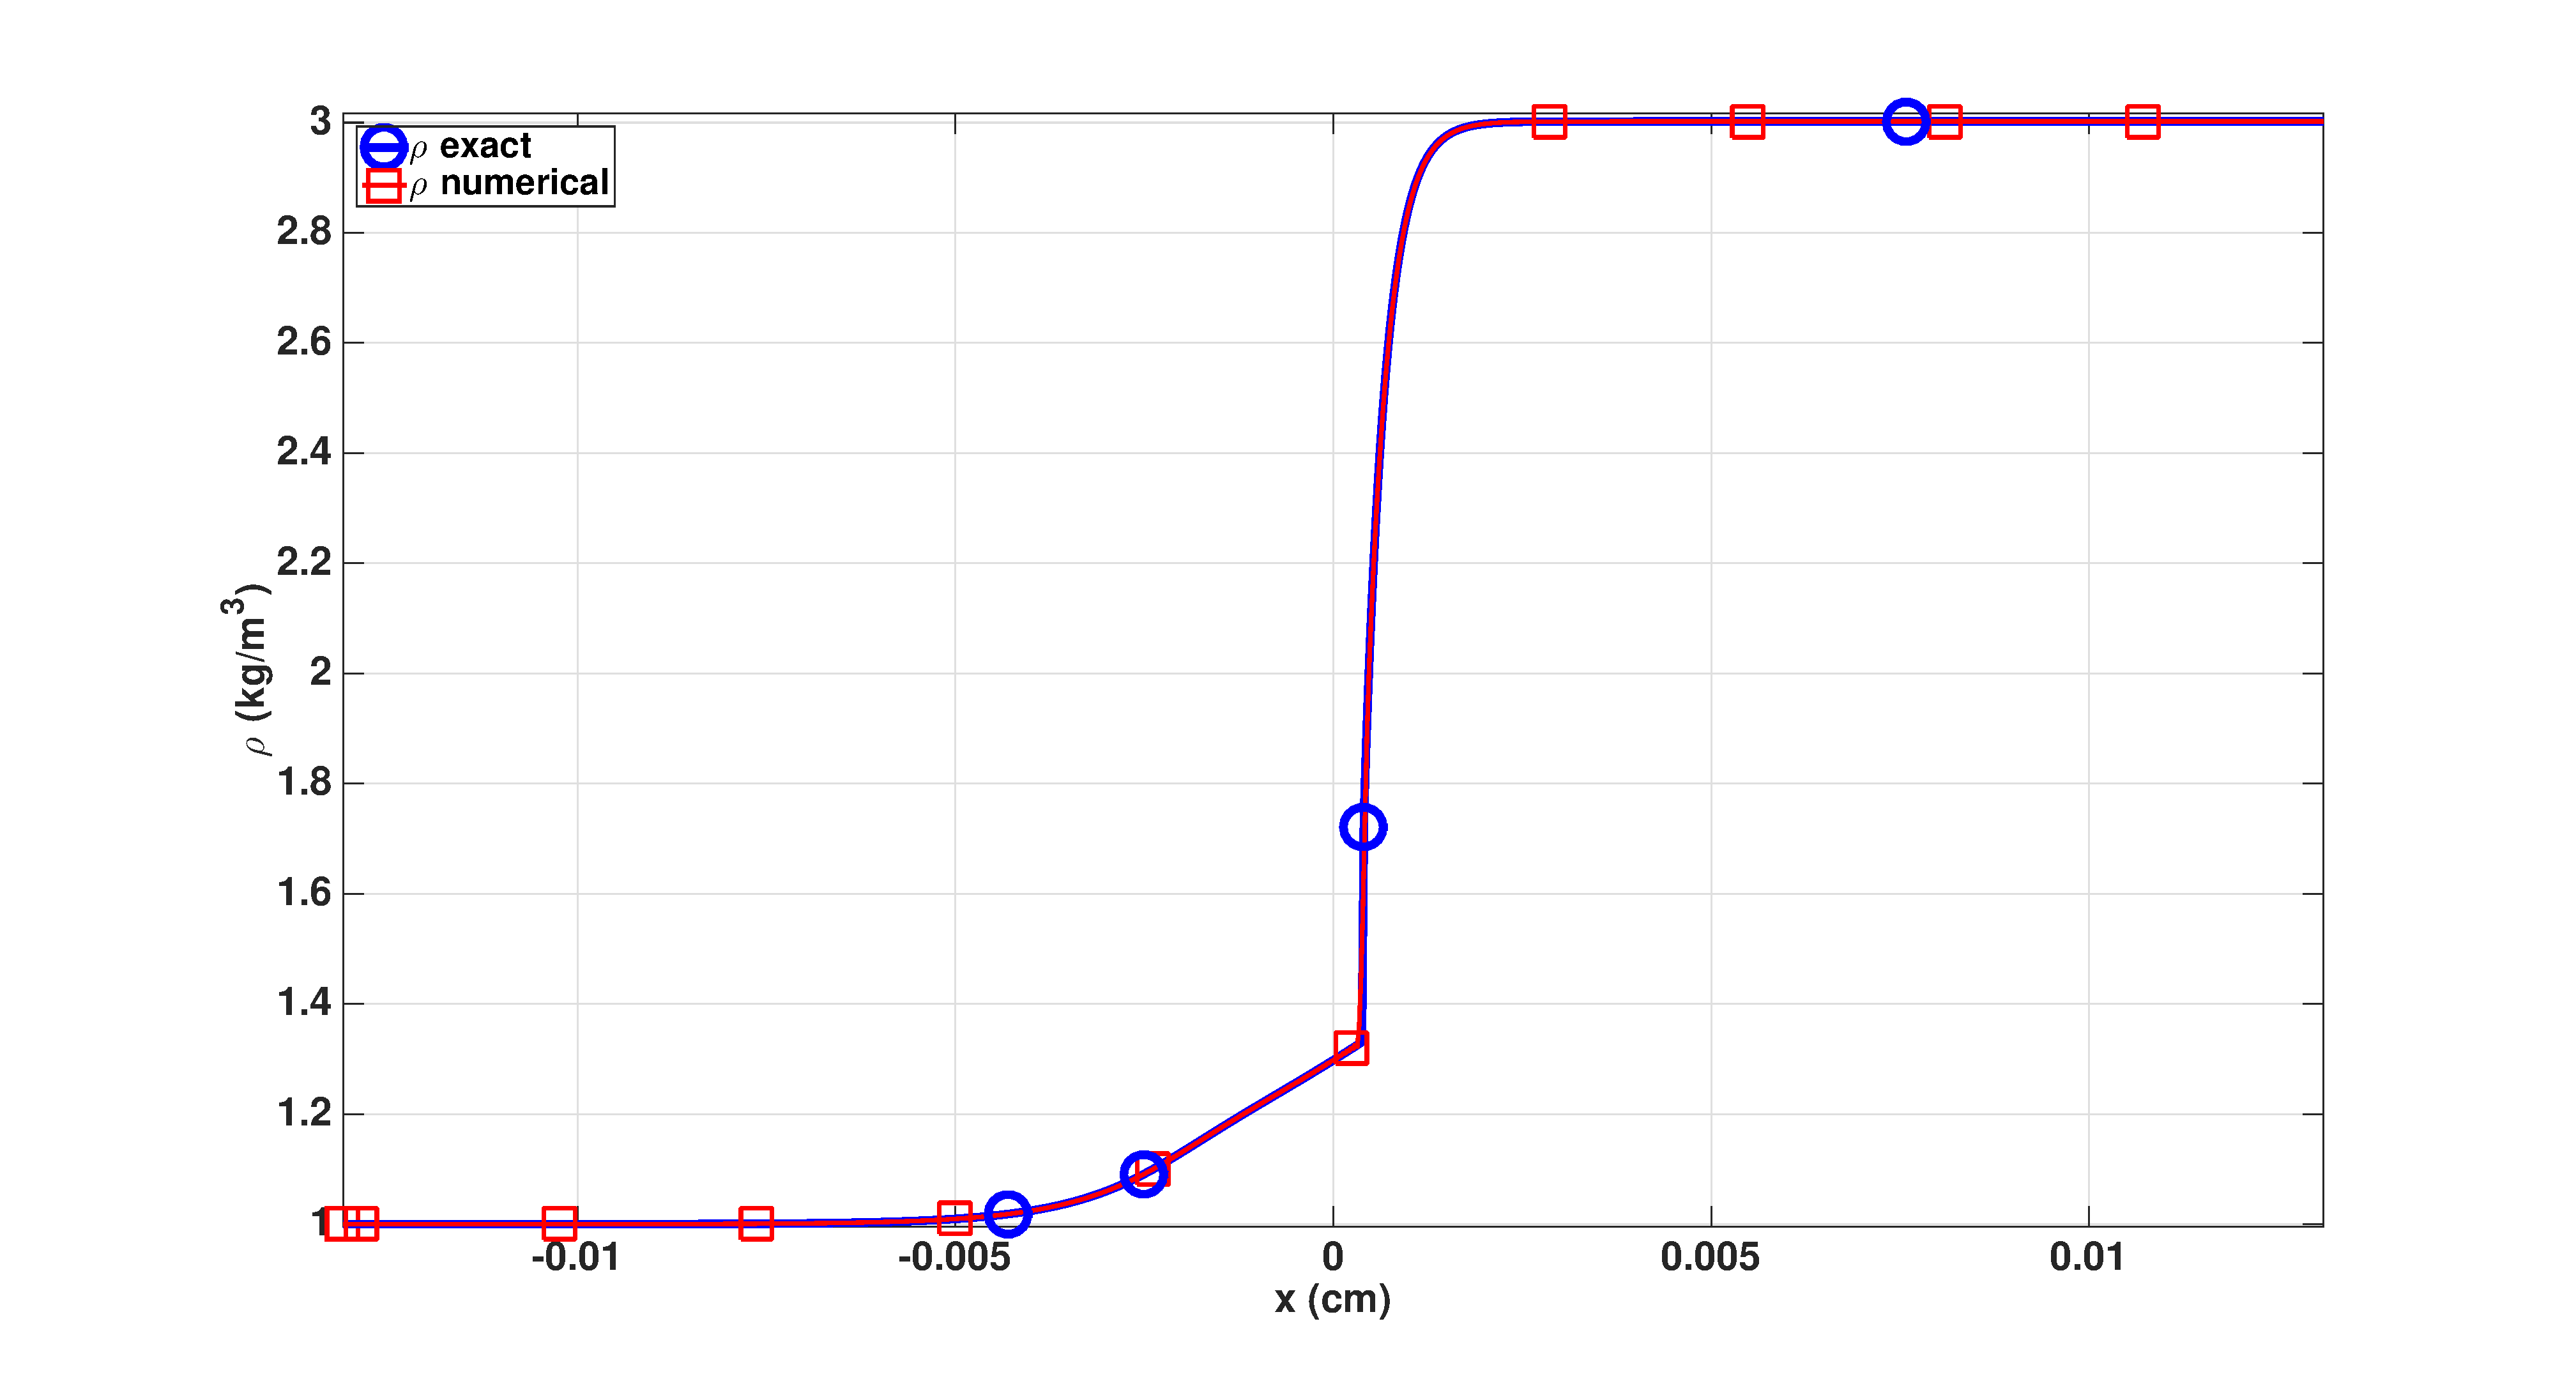
\includegraphics[width=\textwidth]{figures/cst-xs/mach_3_cst_xs_nel_1000_density.eps}
    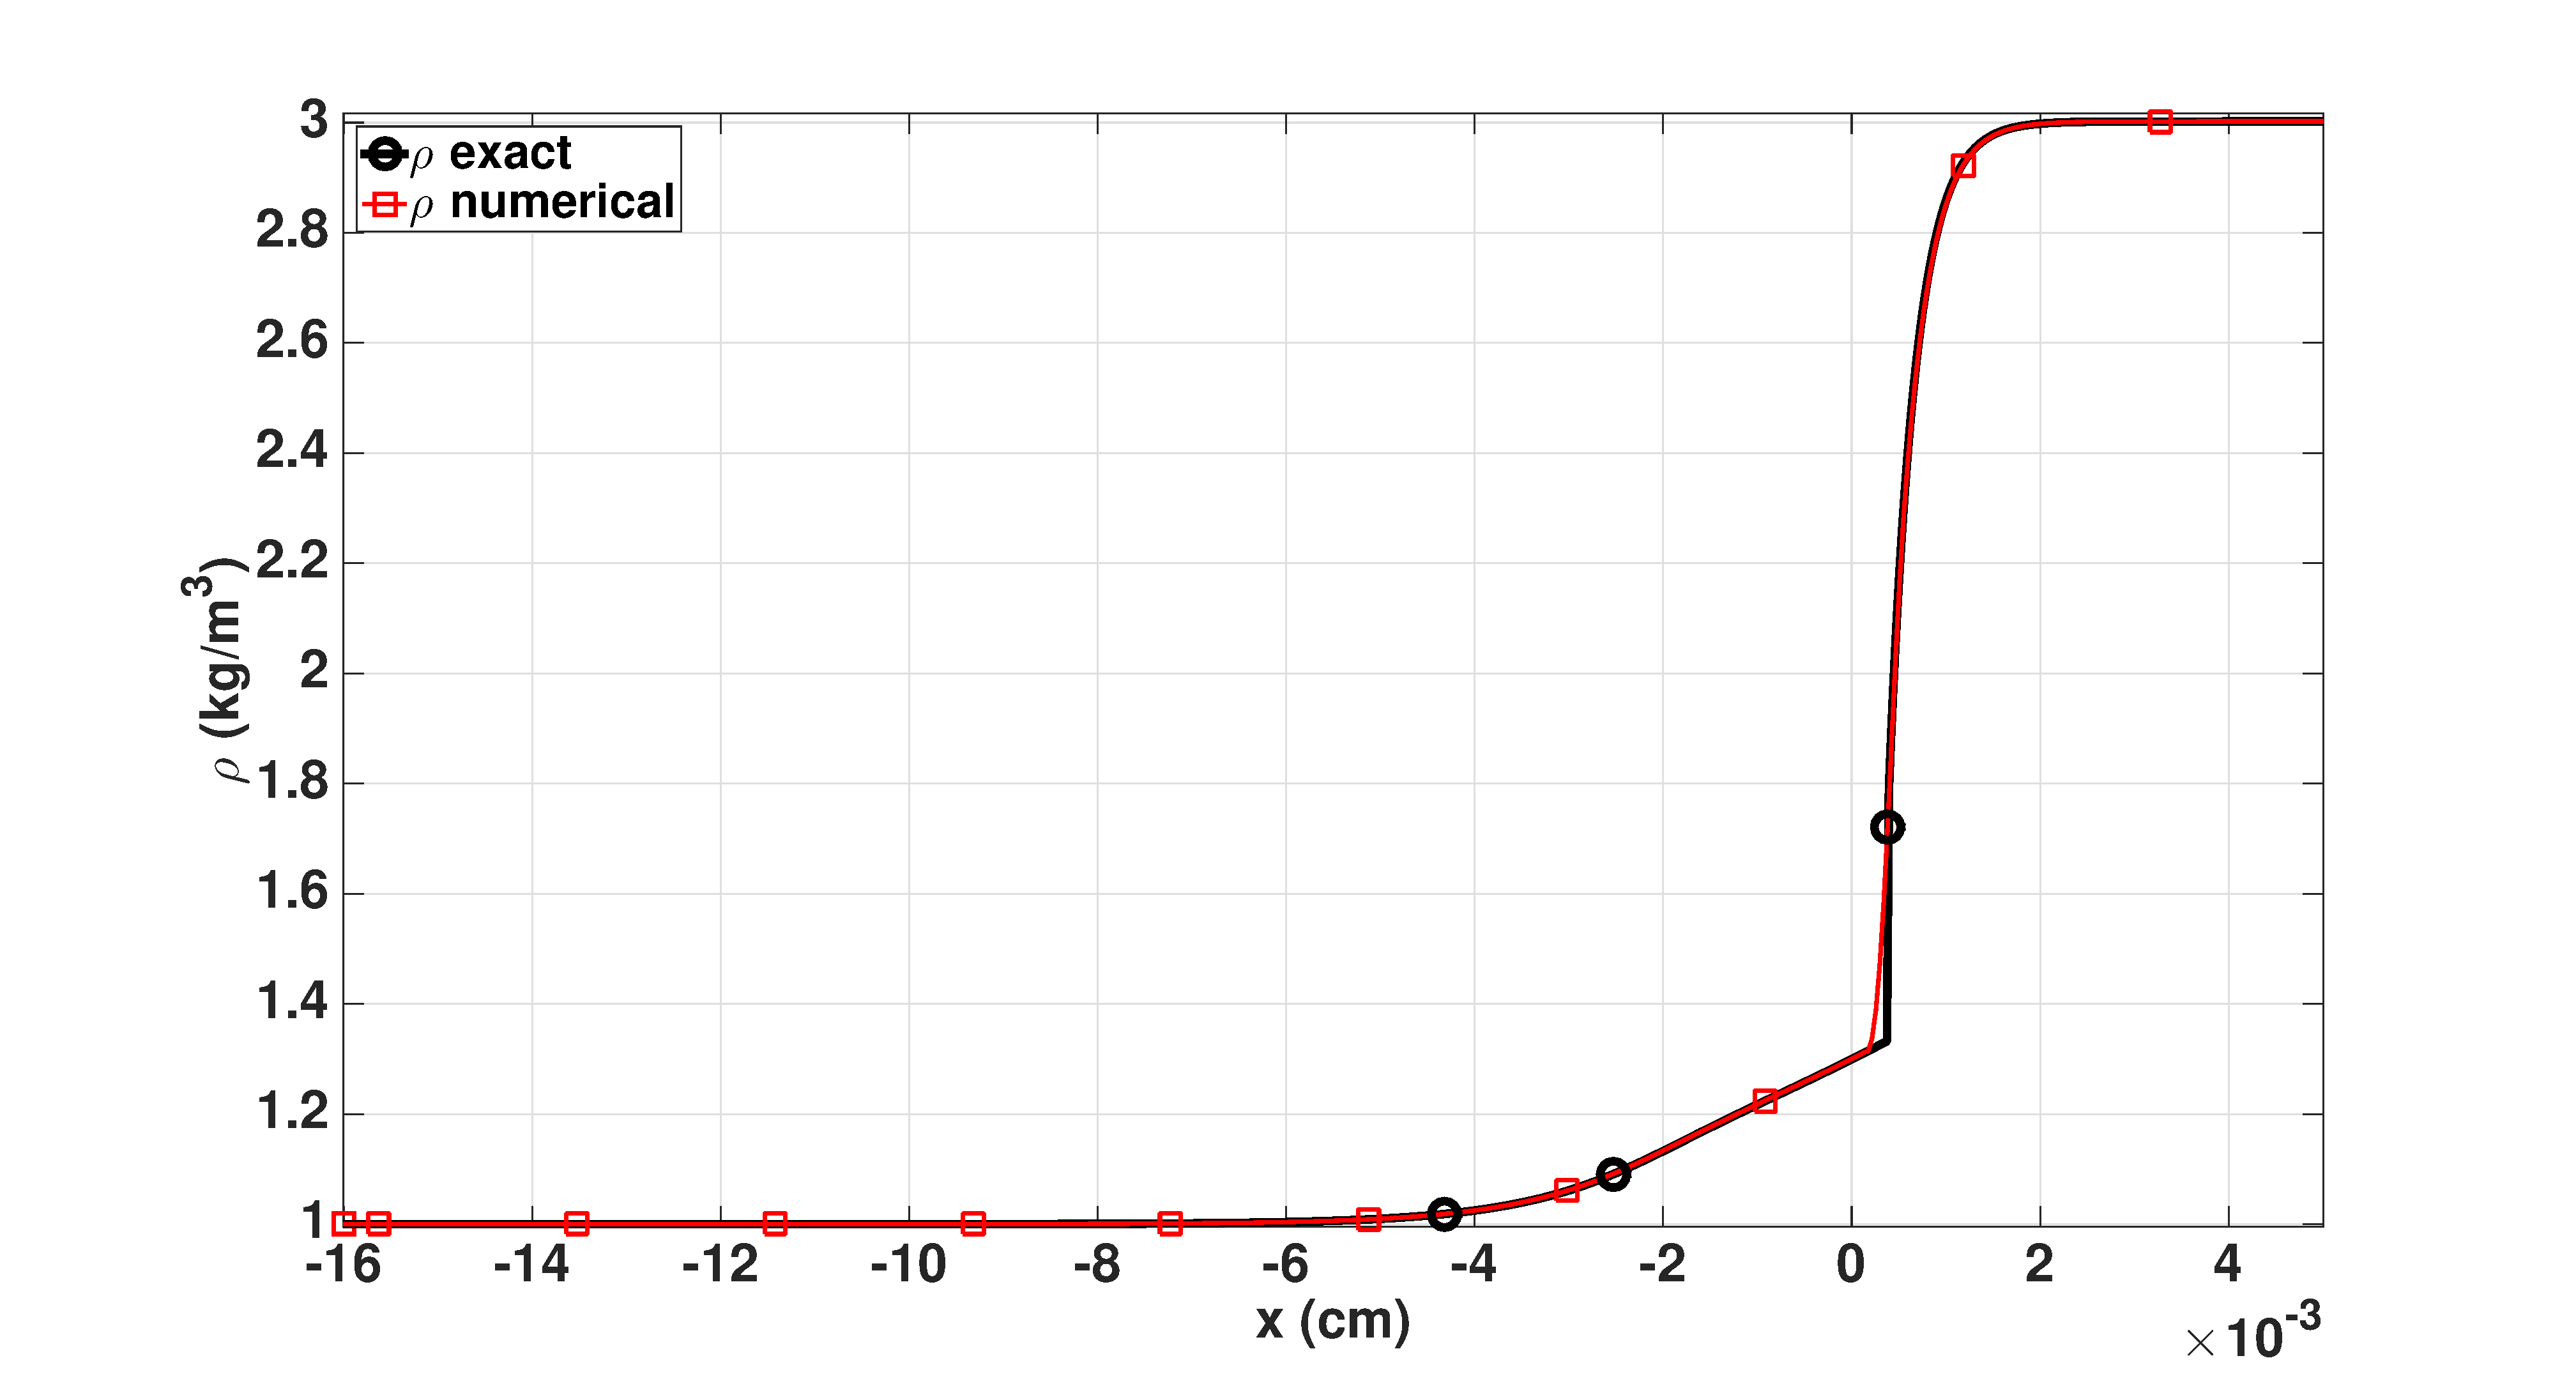
\includegraphics[width=\textwidth]{figures/cst-xs/mach_3_cst_xs_nel_500_density.eps}    
    \caption{Steady-state solution of the material density for the Mach 3 shock test.}\label{fig:mach-3-cst-xs-dens}
\end{figure}
%
\begin{figure}[H]
    \centering
%    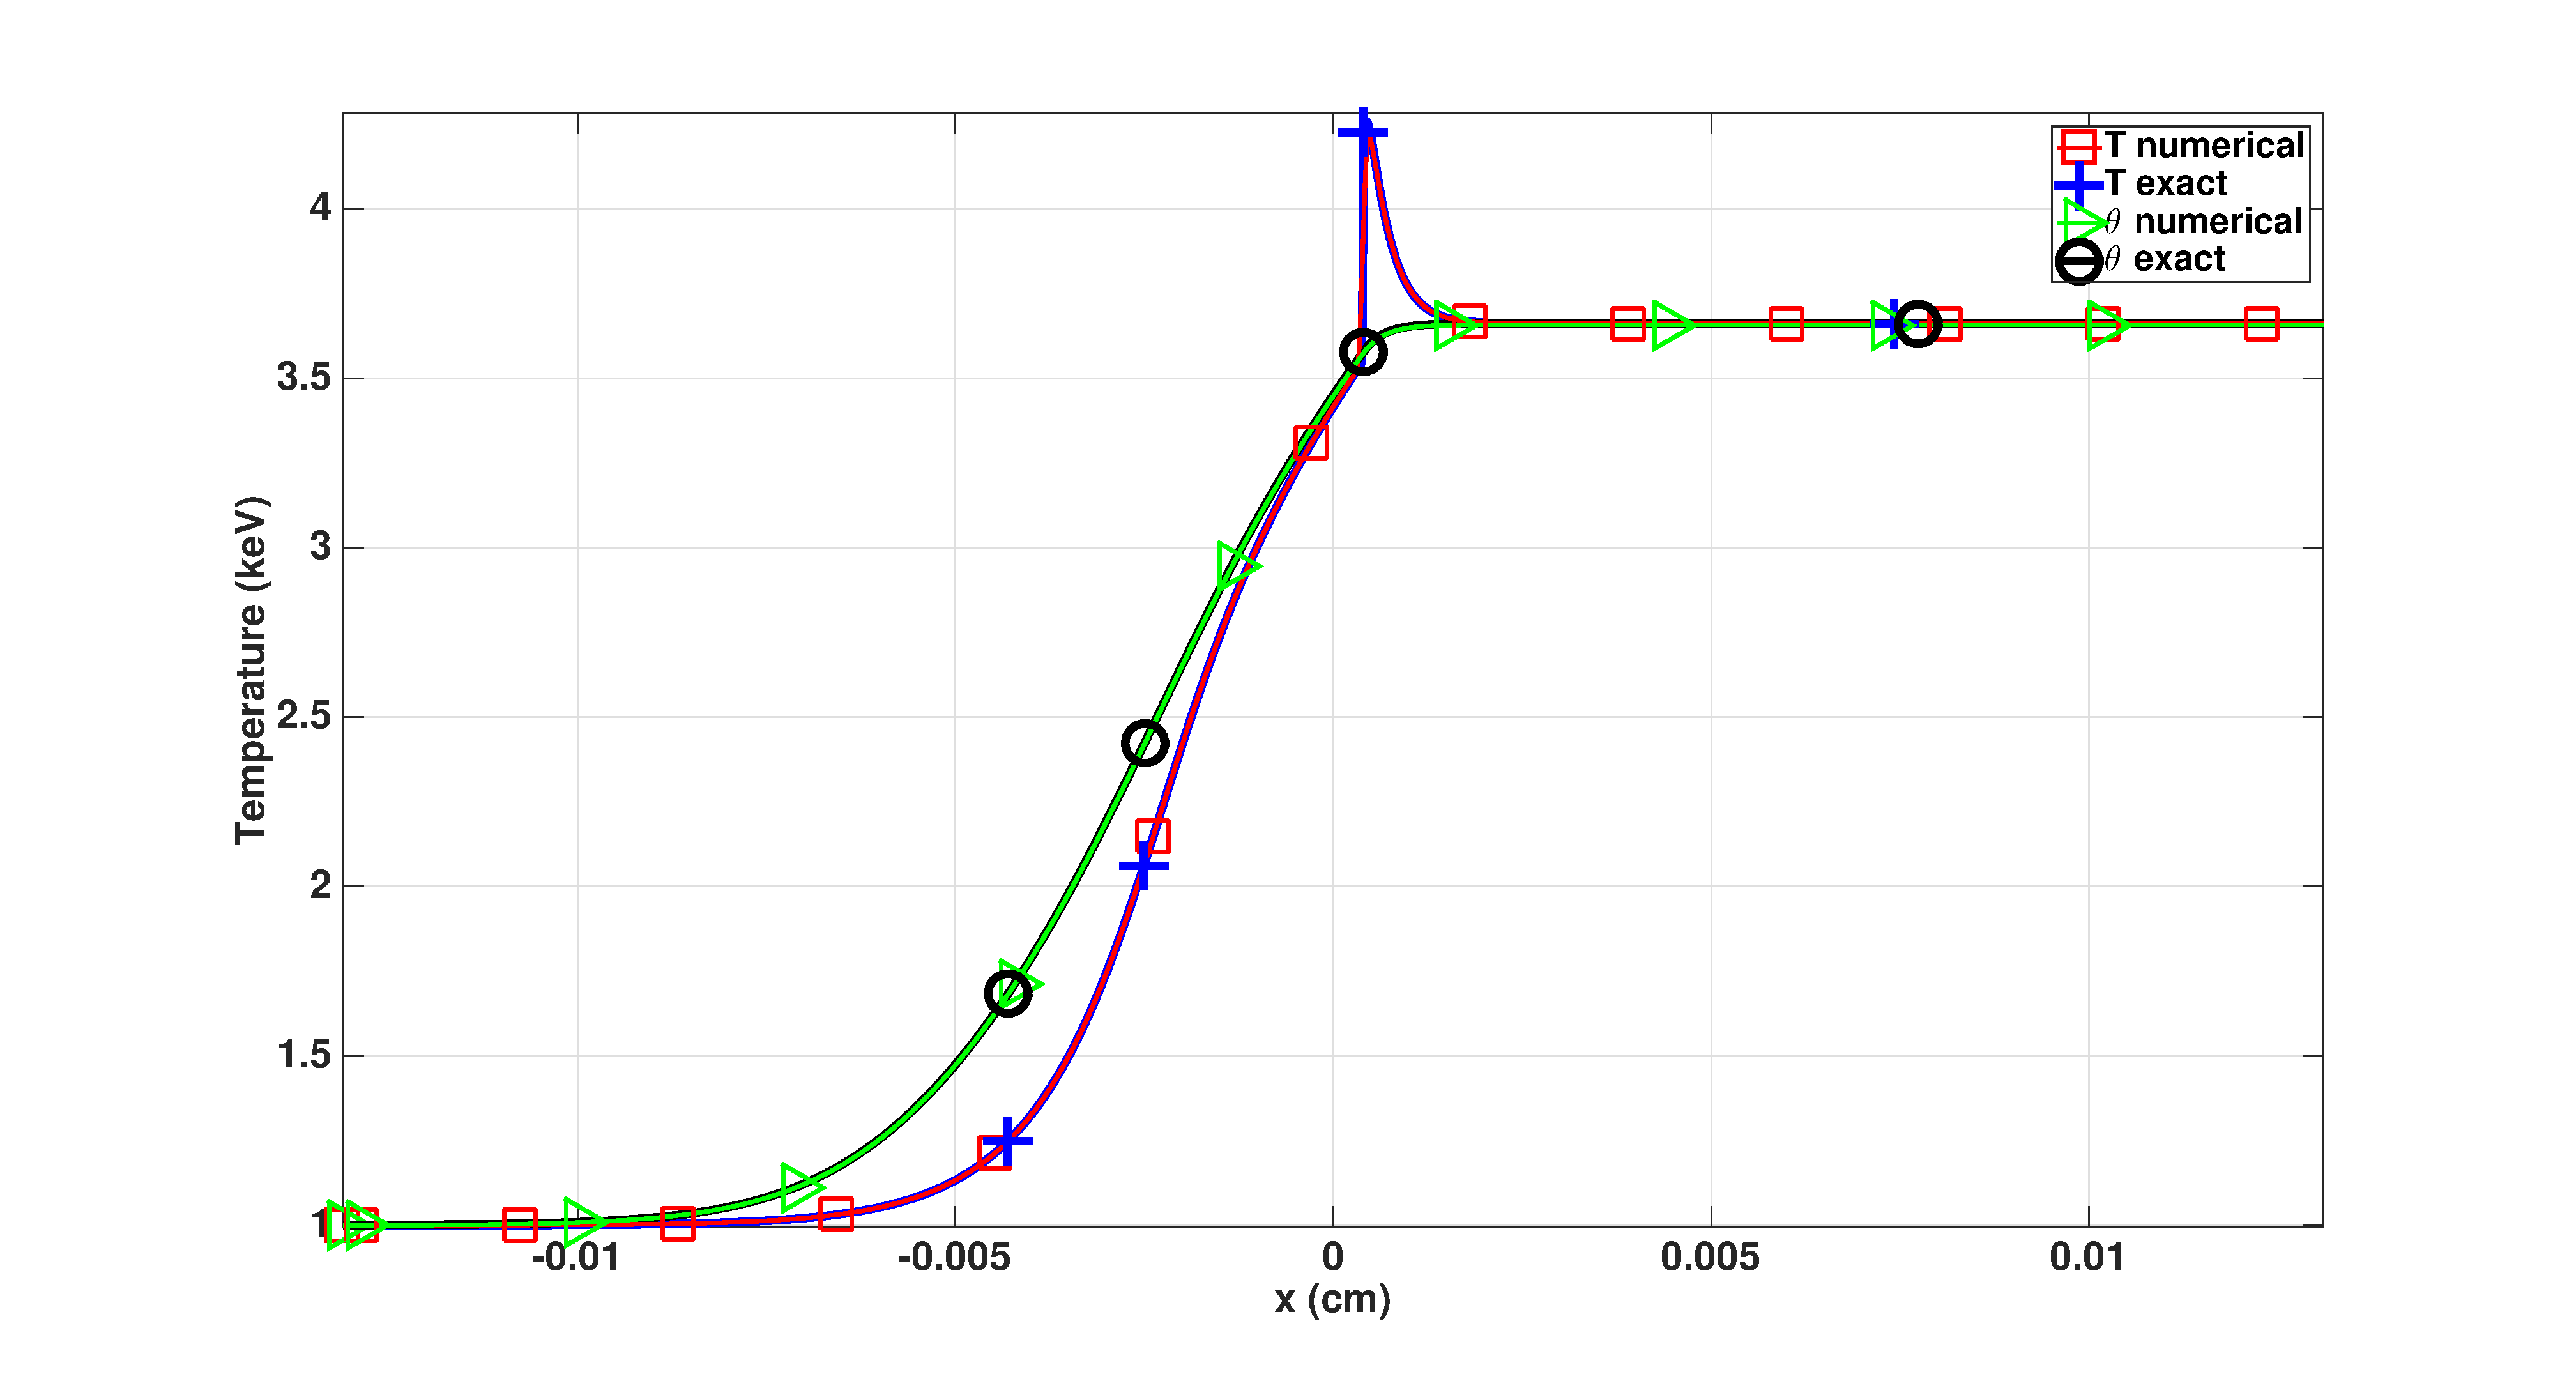
\includegraphics[width=\textwidth]{figures/cst-xs/mach_3_cst_xs_nel_1000_temperature.eps}
    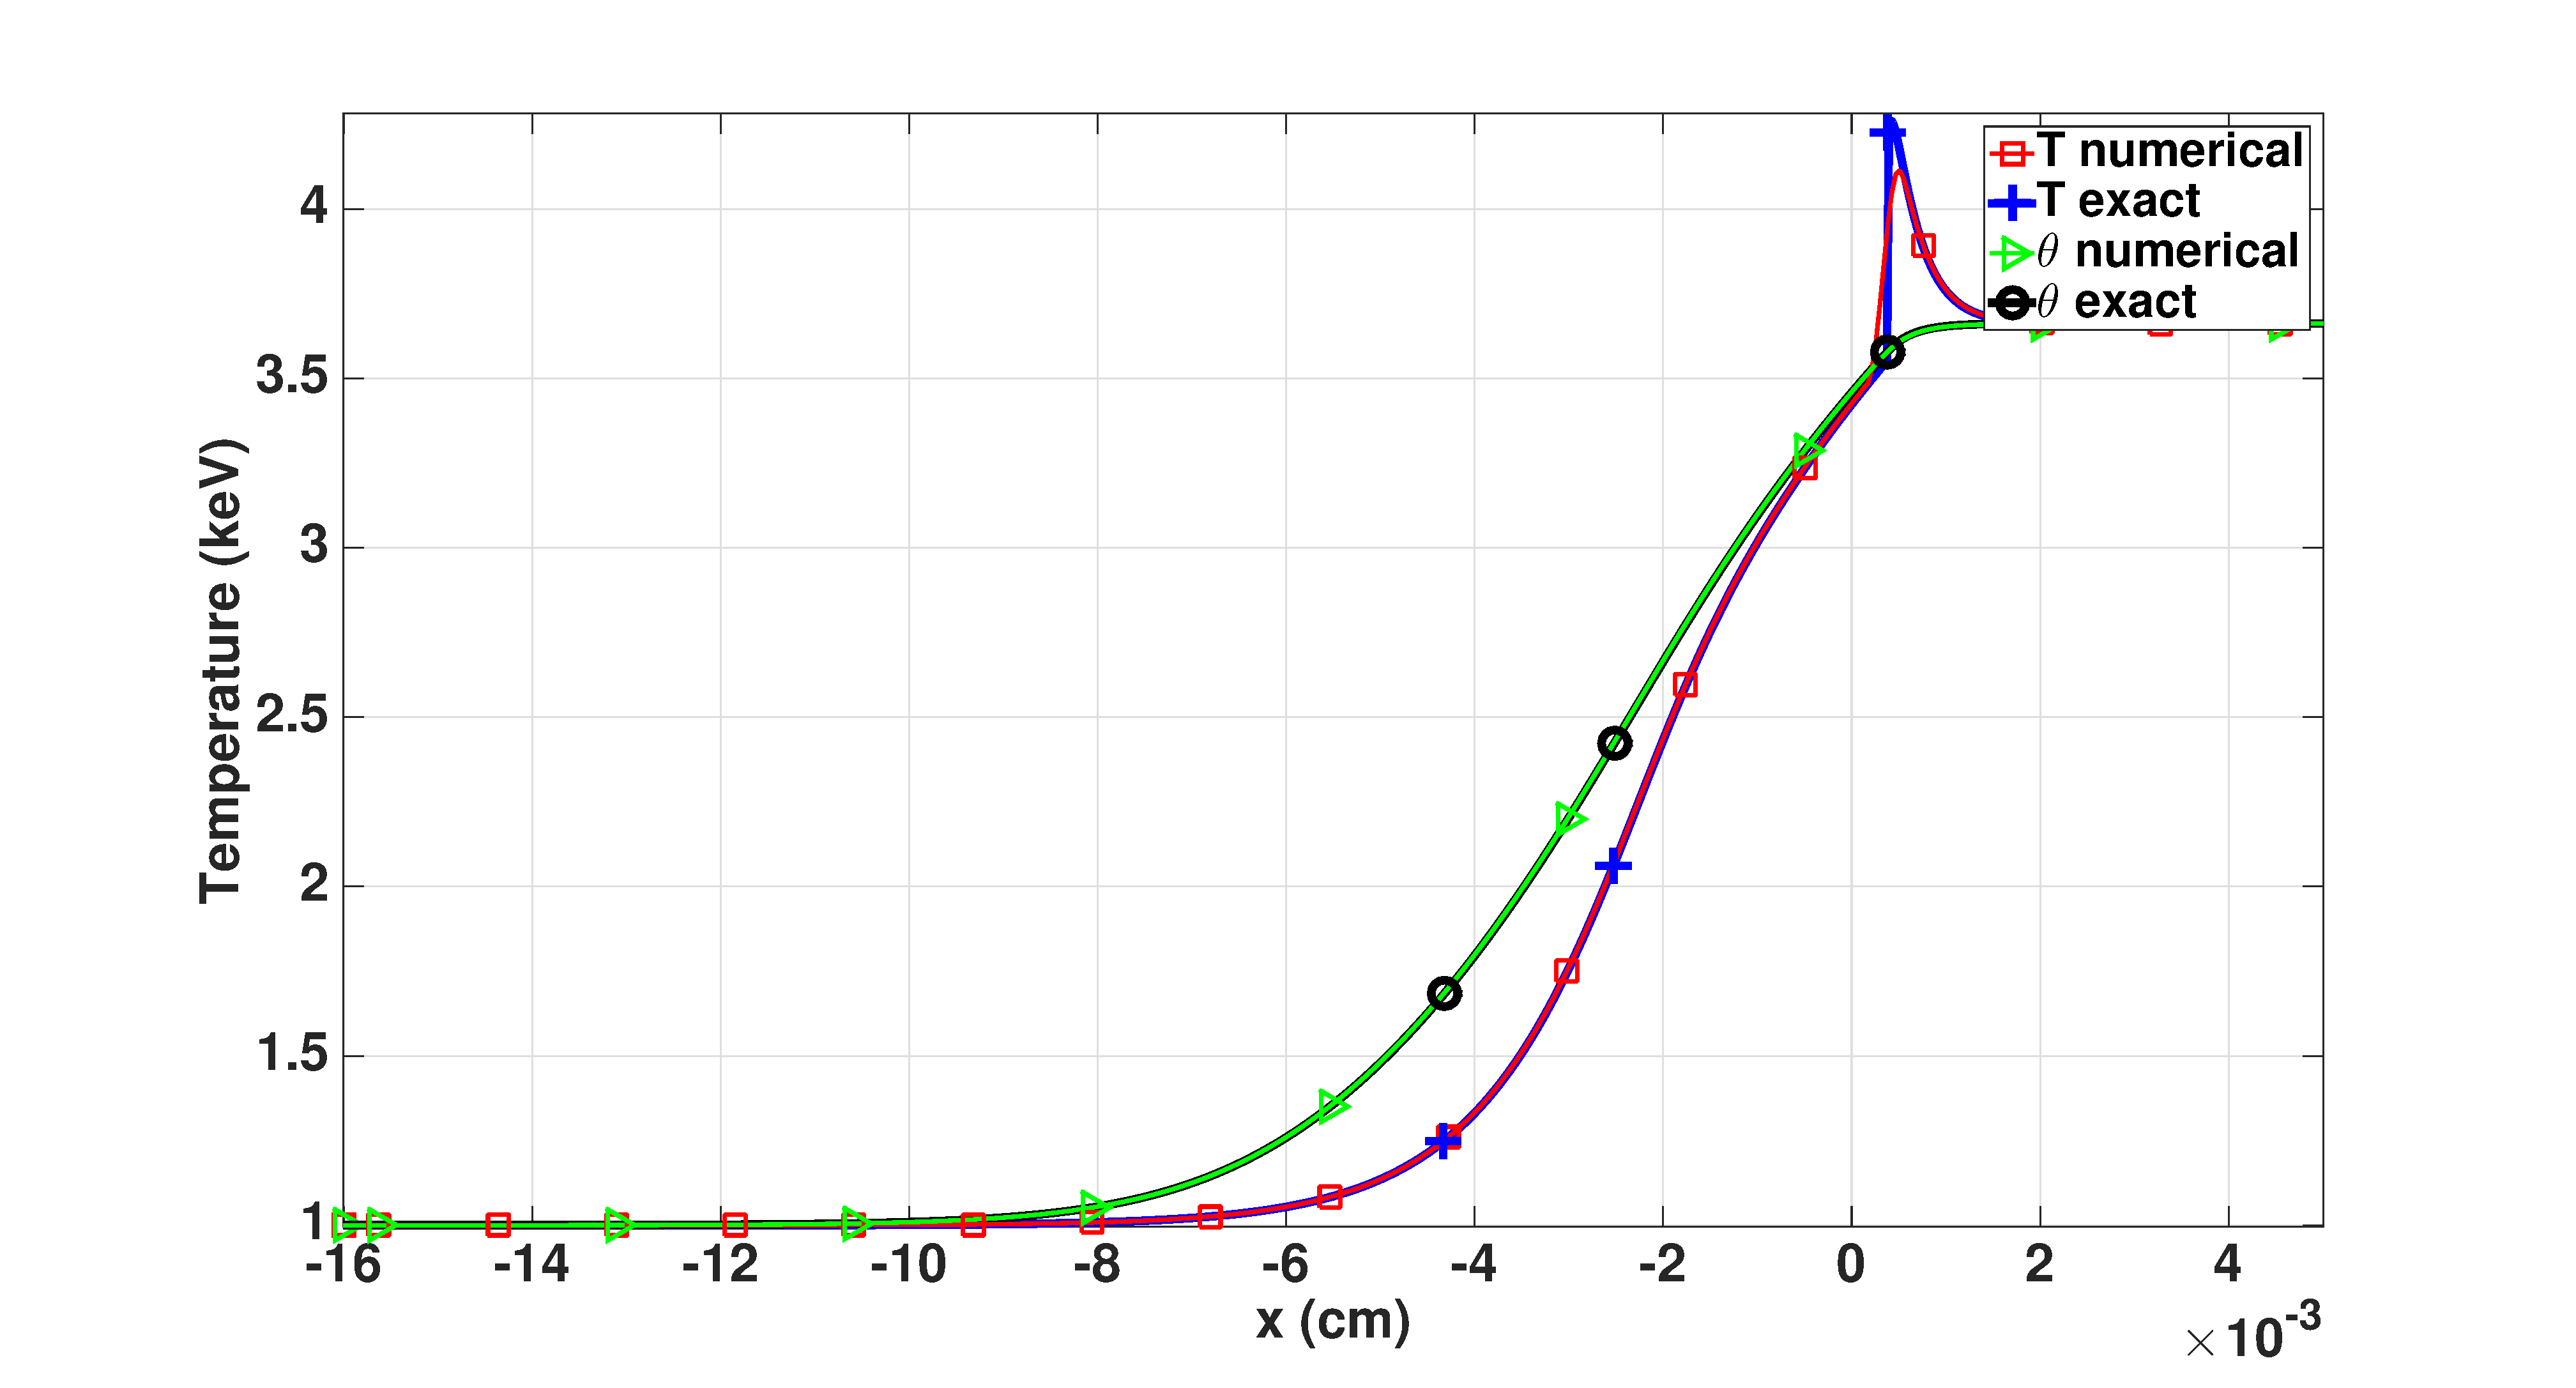
\includegraphics[width=\textwidth]{figures/cst-xs/mach_3_cst_xs_nel_500_temperature.eps}    
    \caption{Steady-state solution of the material and radiation temperatures for the Mach 3 shock test.}\label{fig:mach-3-cst-xs-temp}
\end{figure}
%
\begin{figure}[H]
    \centering
%    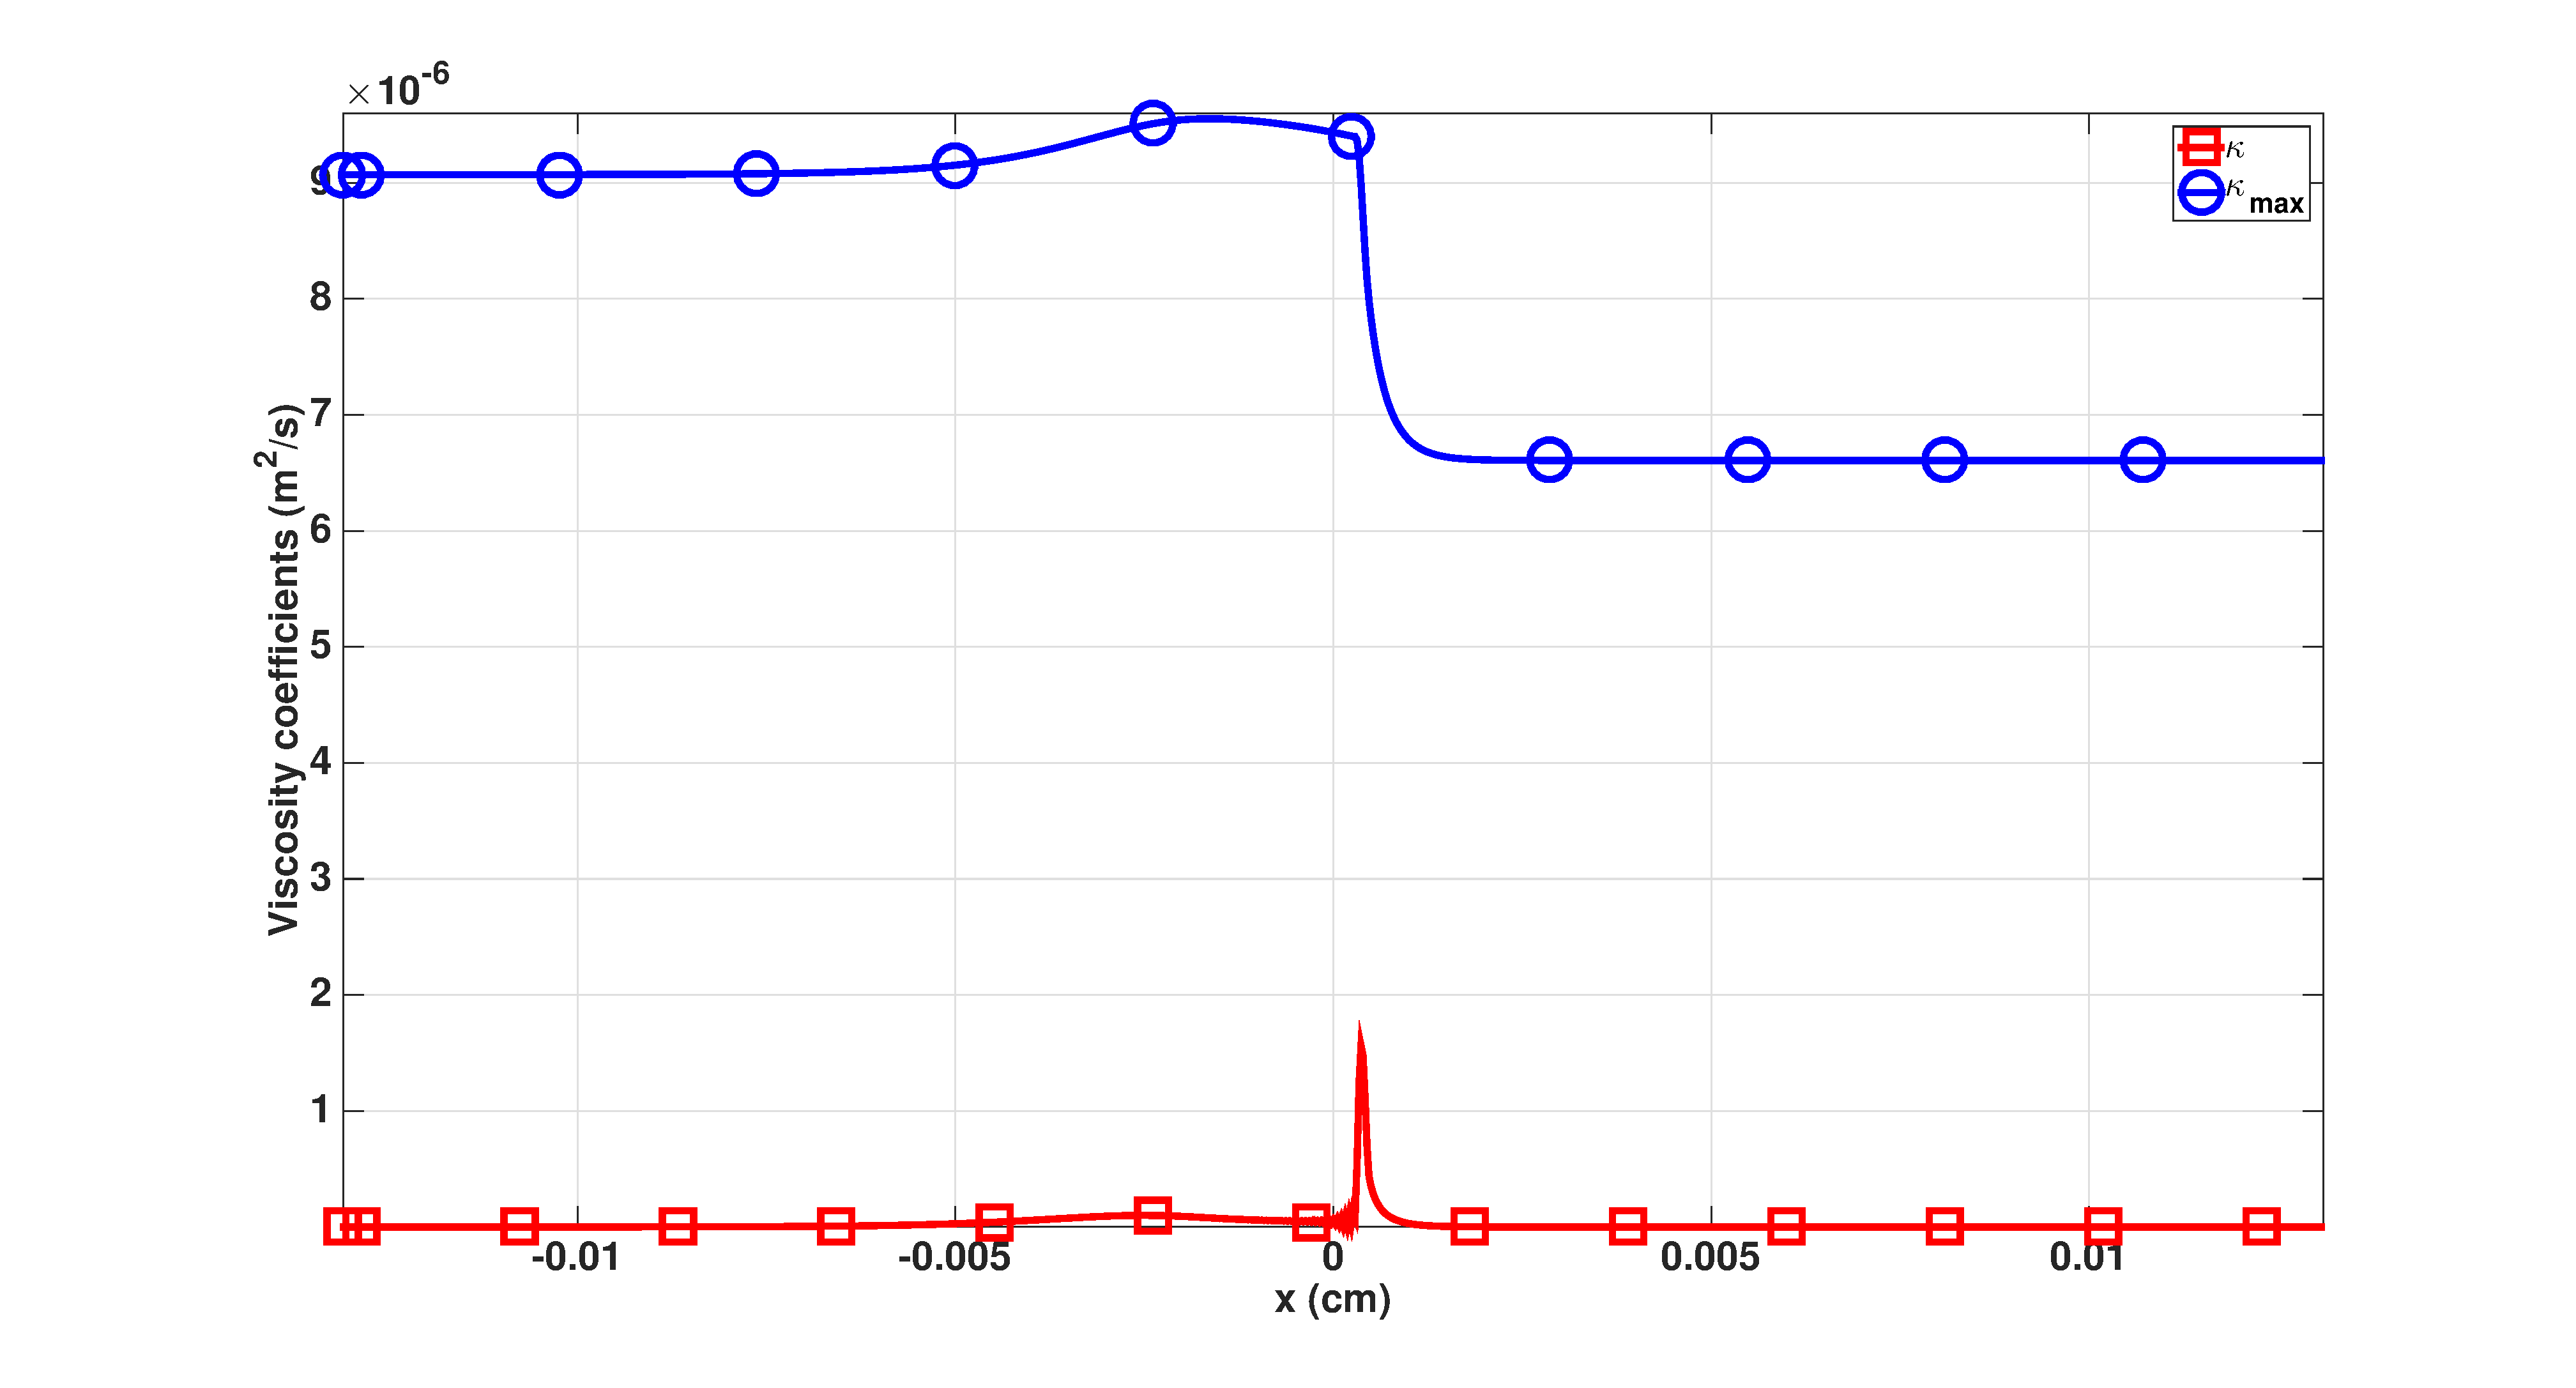
\includegraphics[width=\textwidth]{figures/cst-xs/mach_3_cst_xs_nel_1000_viscosity.eps}
    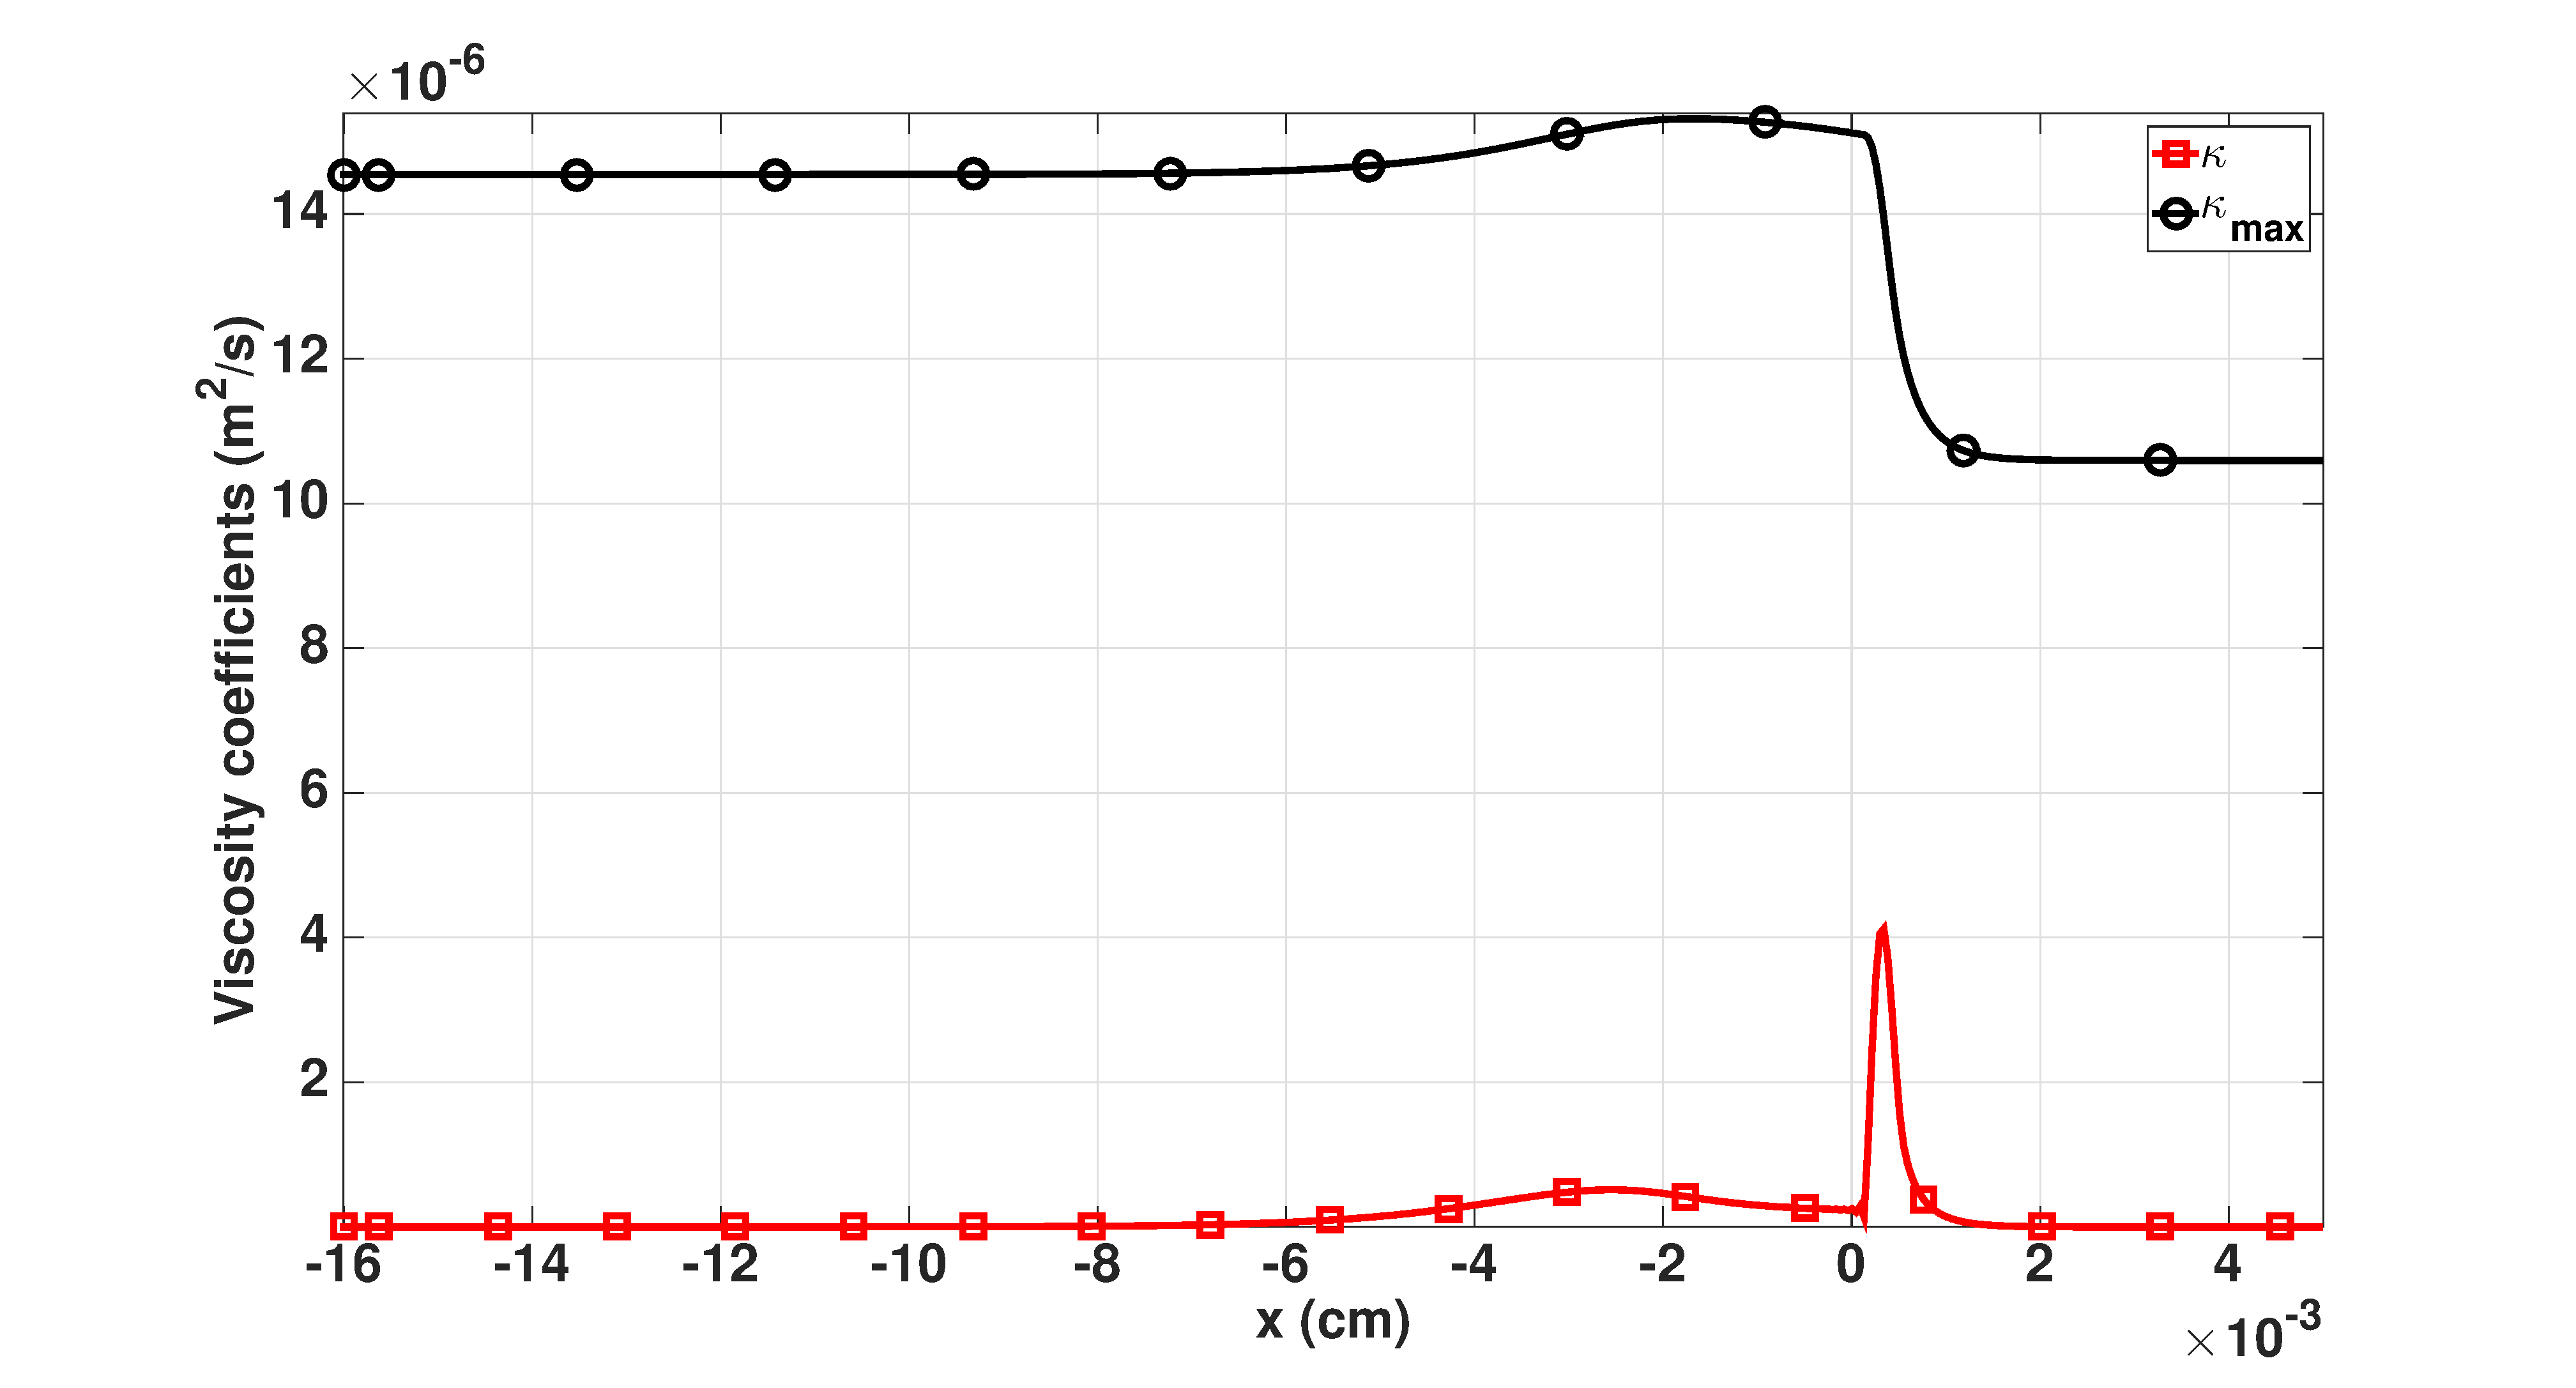
\includegraphics[width=\textwidth]{figures/cst-xs/mach_3_cst_xs_nel_500_viscosity.eps}    
    \caption{Steady-state solution of the artificial viscosity coefficients for the Mach 3 shock test.}\label{fig:mach-3-cst-xs-visc}
\end{figure}
%
%------------------------------------------------------------------
\subsection{Mach 3 shock test with temperature-dependent opacities}\label{sec:mach-3-no-cst-xs}
%------------------------------------------------------------------
%
\begin{itemize}
\item numerical results using definition of the viscosity coefficient provided in previous section: density, temperature, opacity and viscosity coefficient profiles.
\item eyeball convergence study when refining the mesh.
\item investigate the influence of the jumps in the definition of the viscosity coefficients: run the same numerical test with and without jumps.
\end{itemize}
%
\begin{figure}[H]
    \centering
    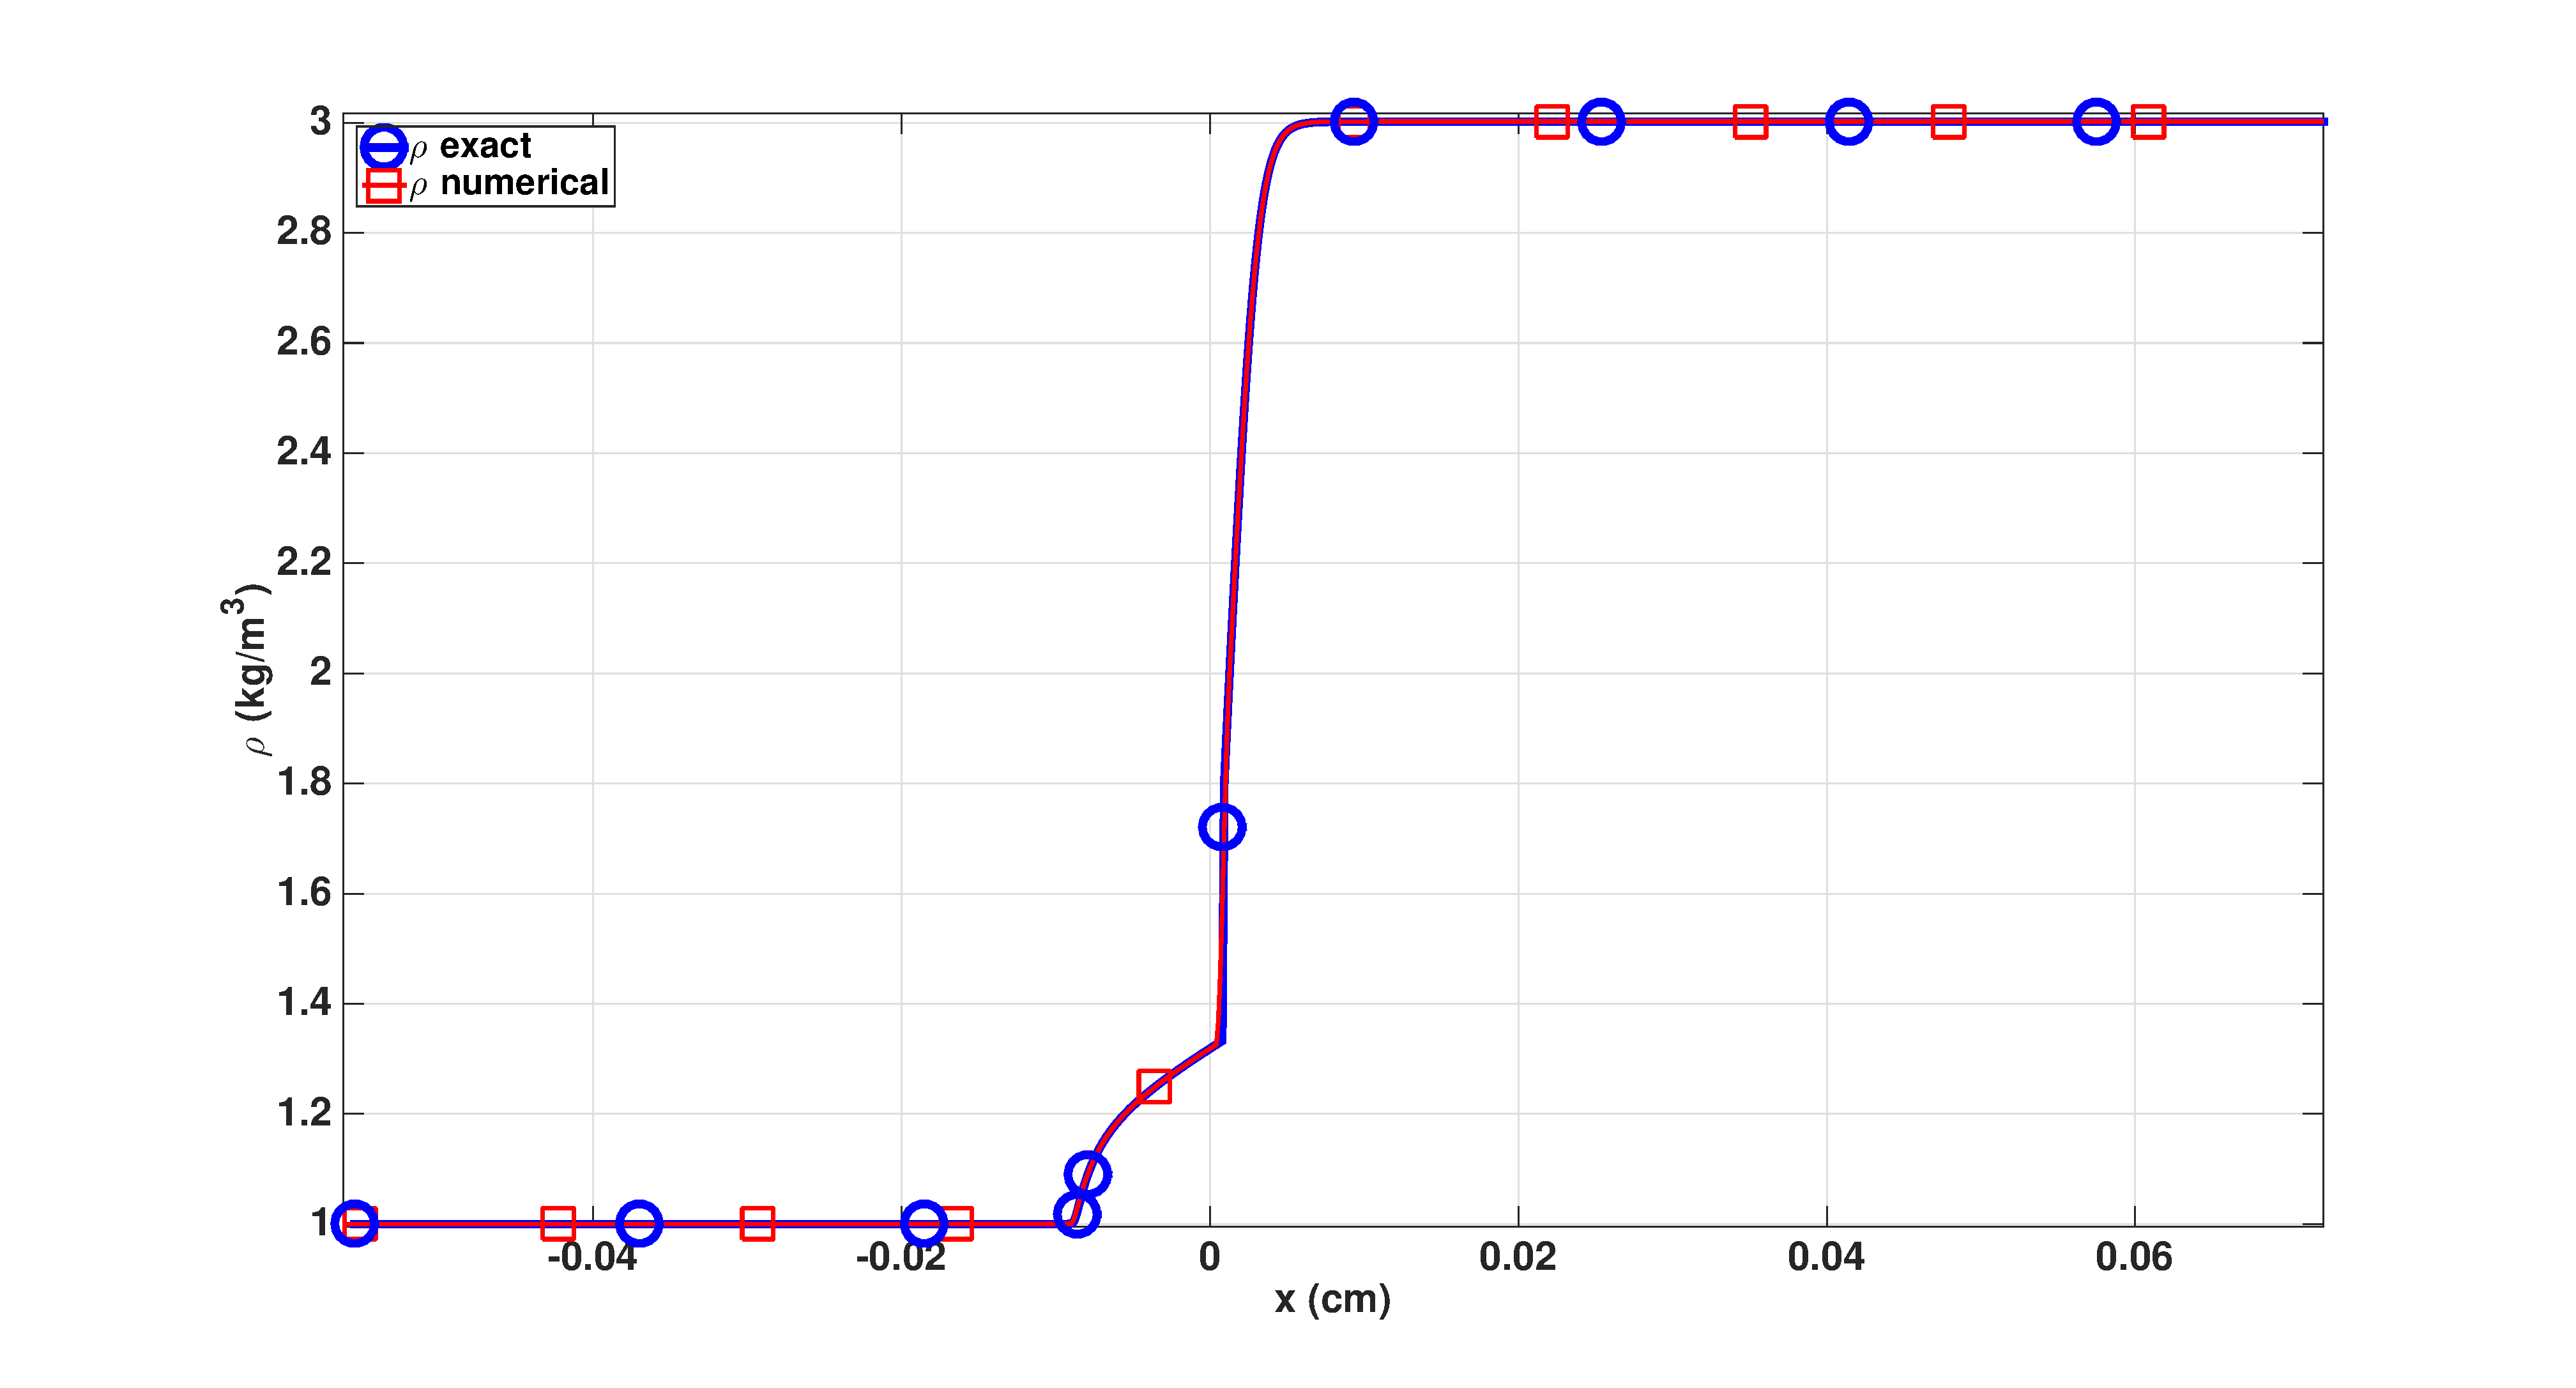
\includegraphics[width=\textwidth]{figures/dpt-xs/mach_3_nel_1000_density.eps}
    \caption{Steady-state solution of the material density for the Mach 3 shock test.}\label{fig:mach-3-dpt-xs-dens}
\end{figure}
%
\begin{figure}[H]
    \centering
    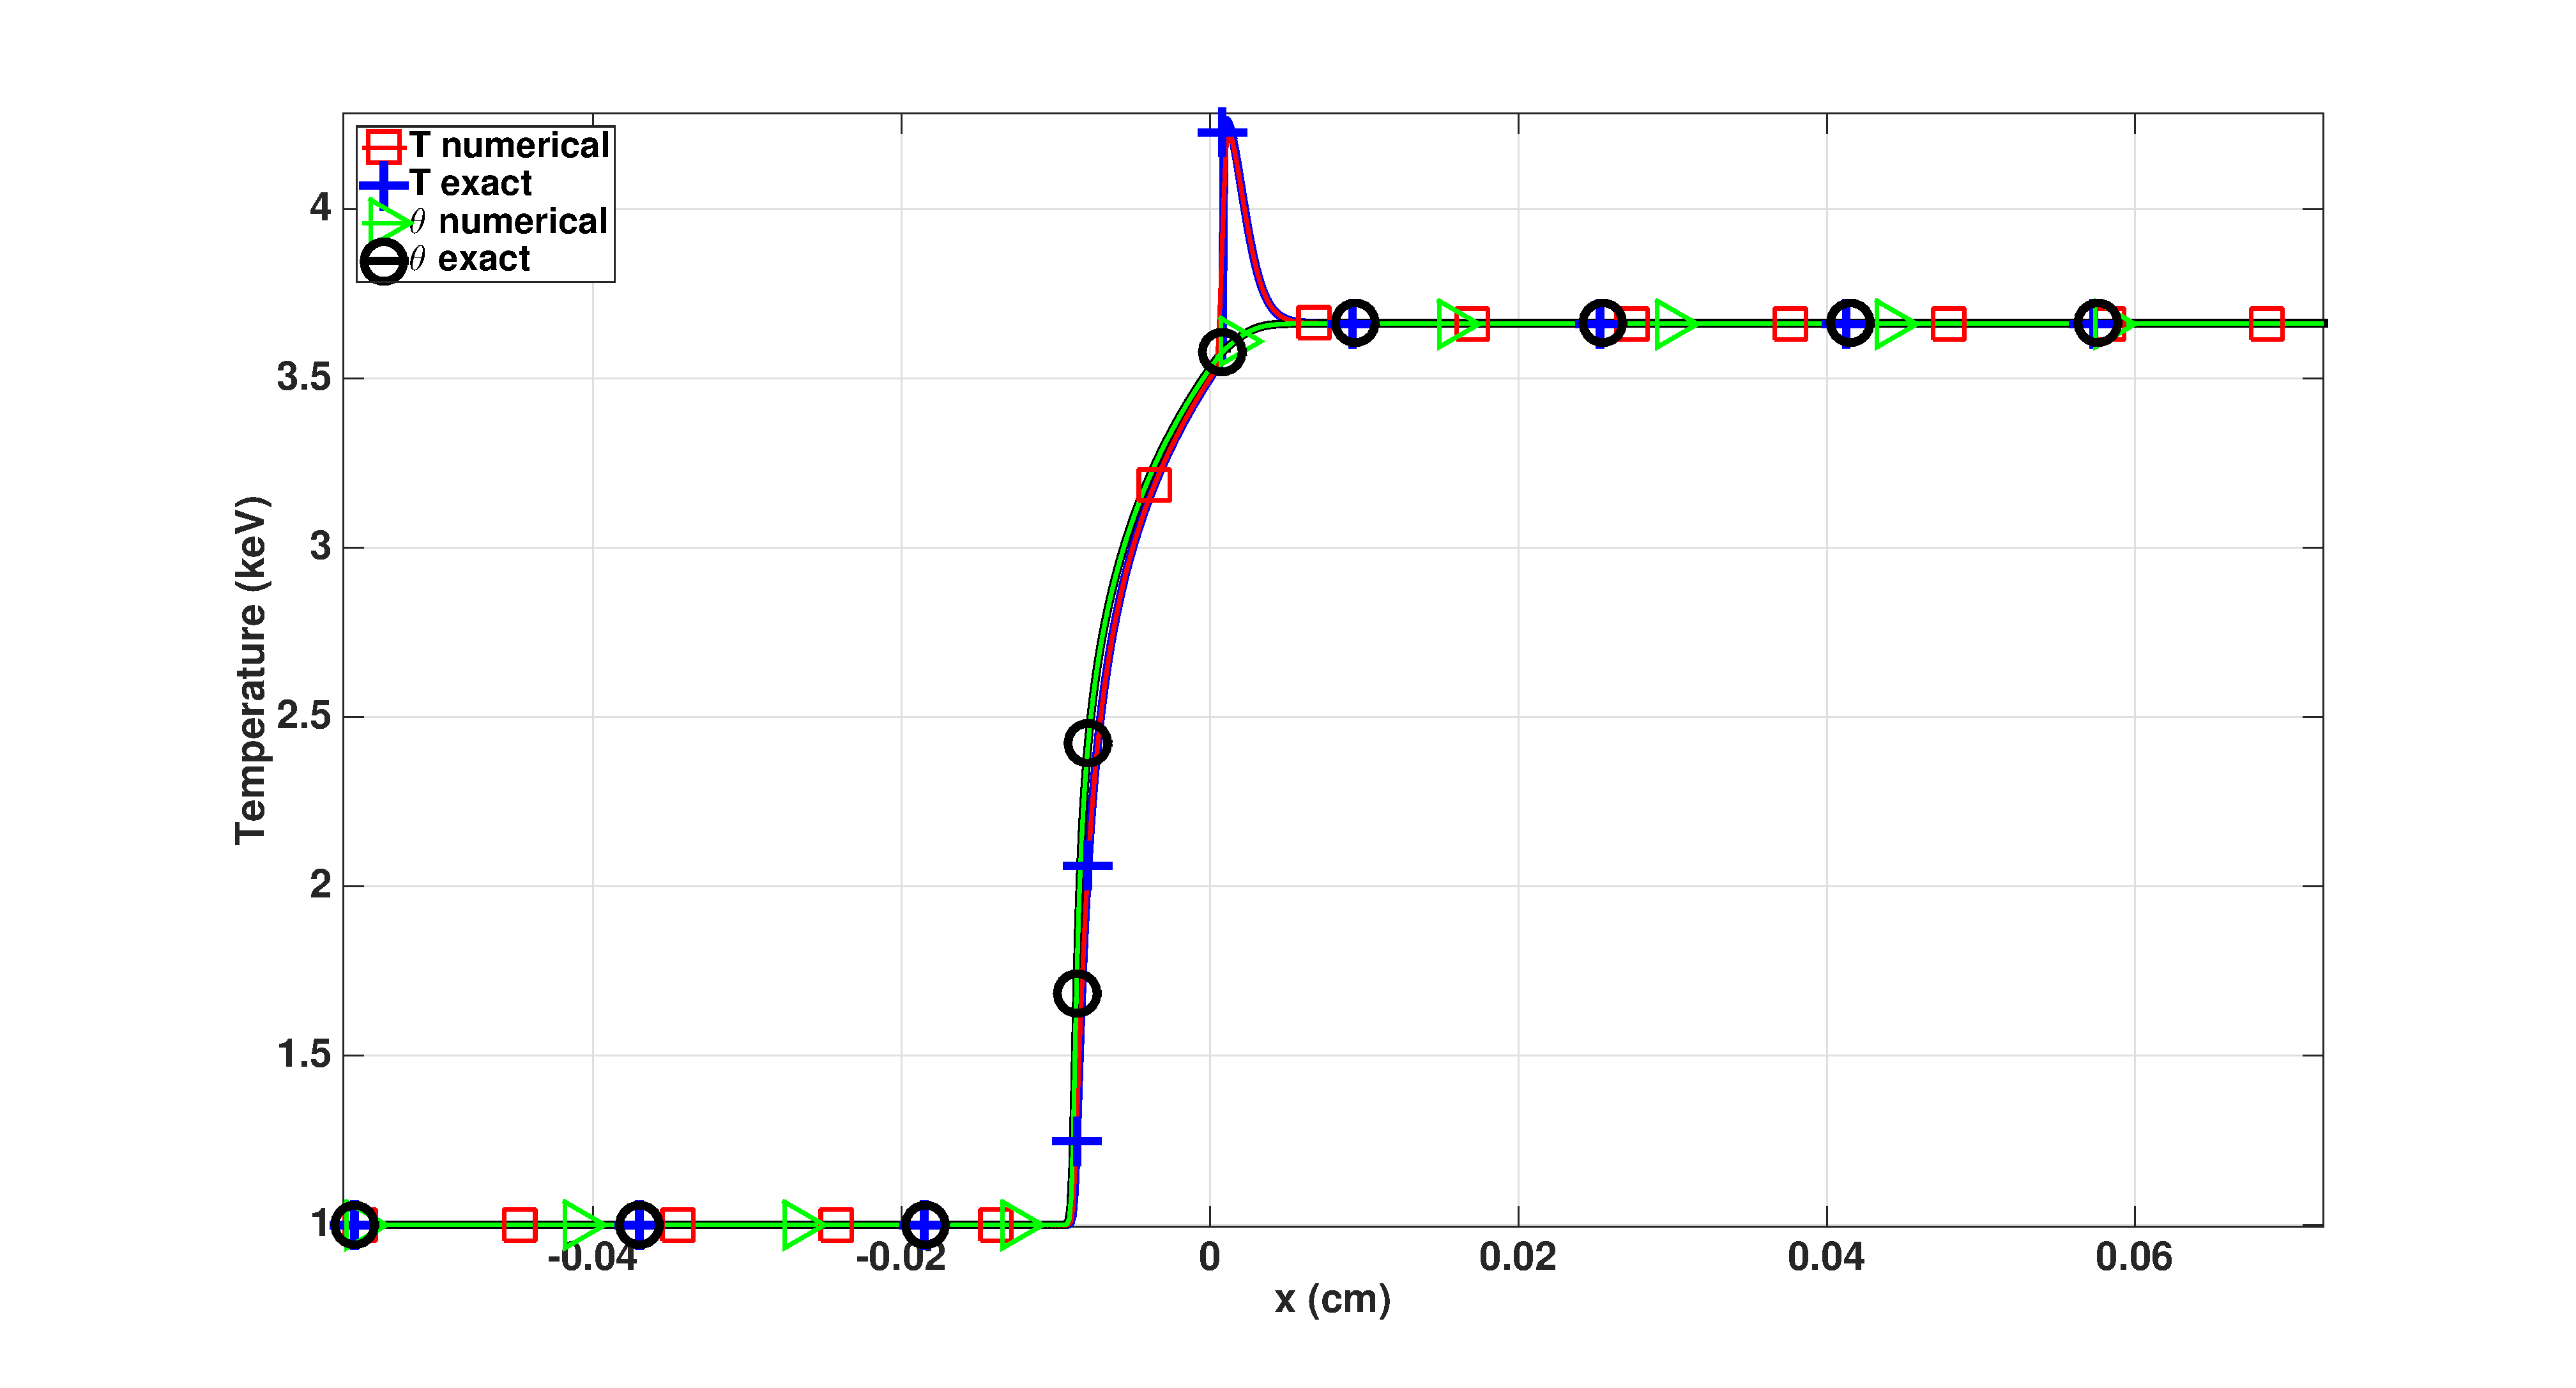
\includegraphics[width=\textwidth]{figures/dpt-xs/mach_3_nel_1000_temperature.eps}
    \caption{Steady-state solution of the material and radiation temperatures for the Mach 3 shock test.}\label{fig:mach-3-dpt-xs-temp}
\end{figure}
%
\begin{figure}[H]
    \centering
    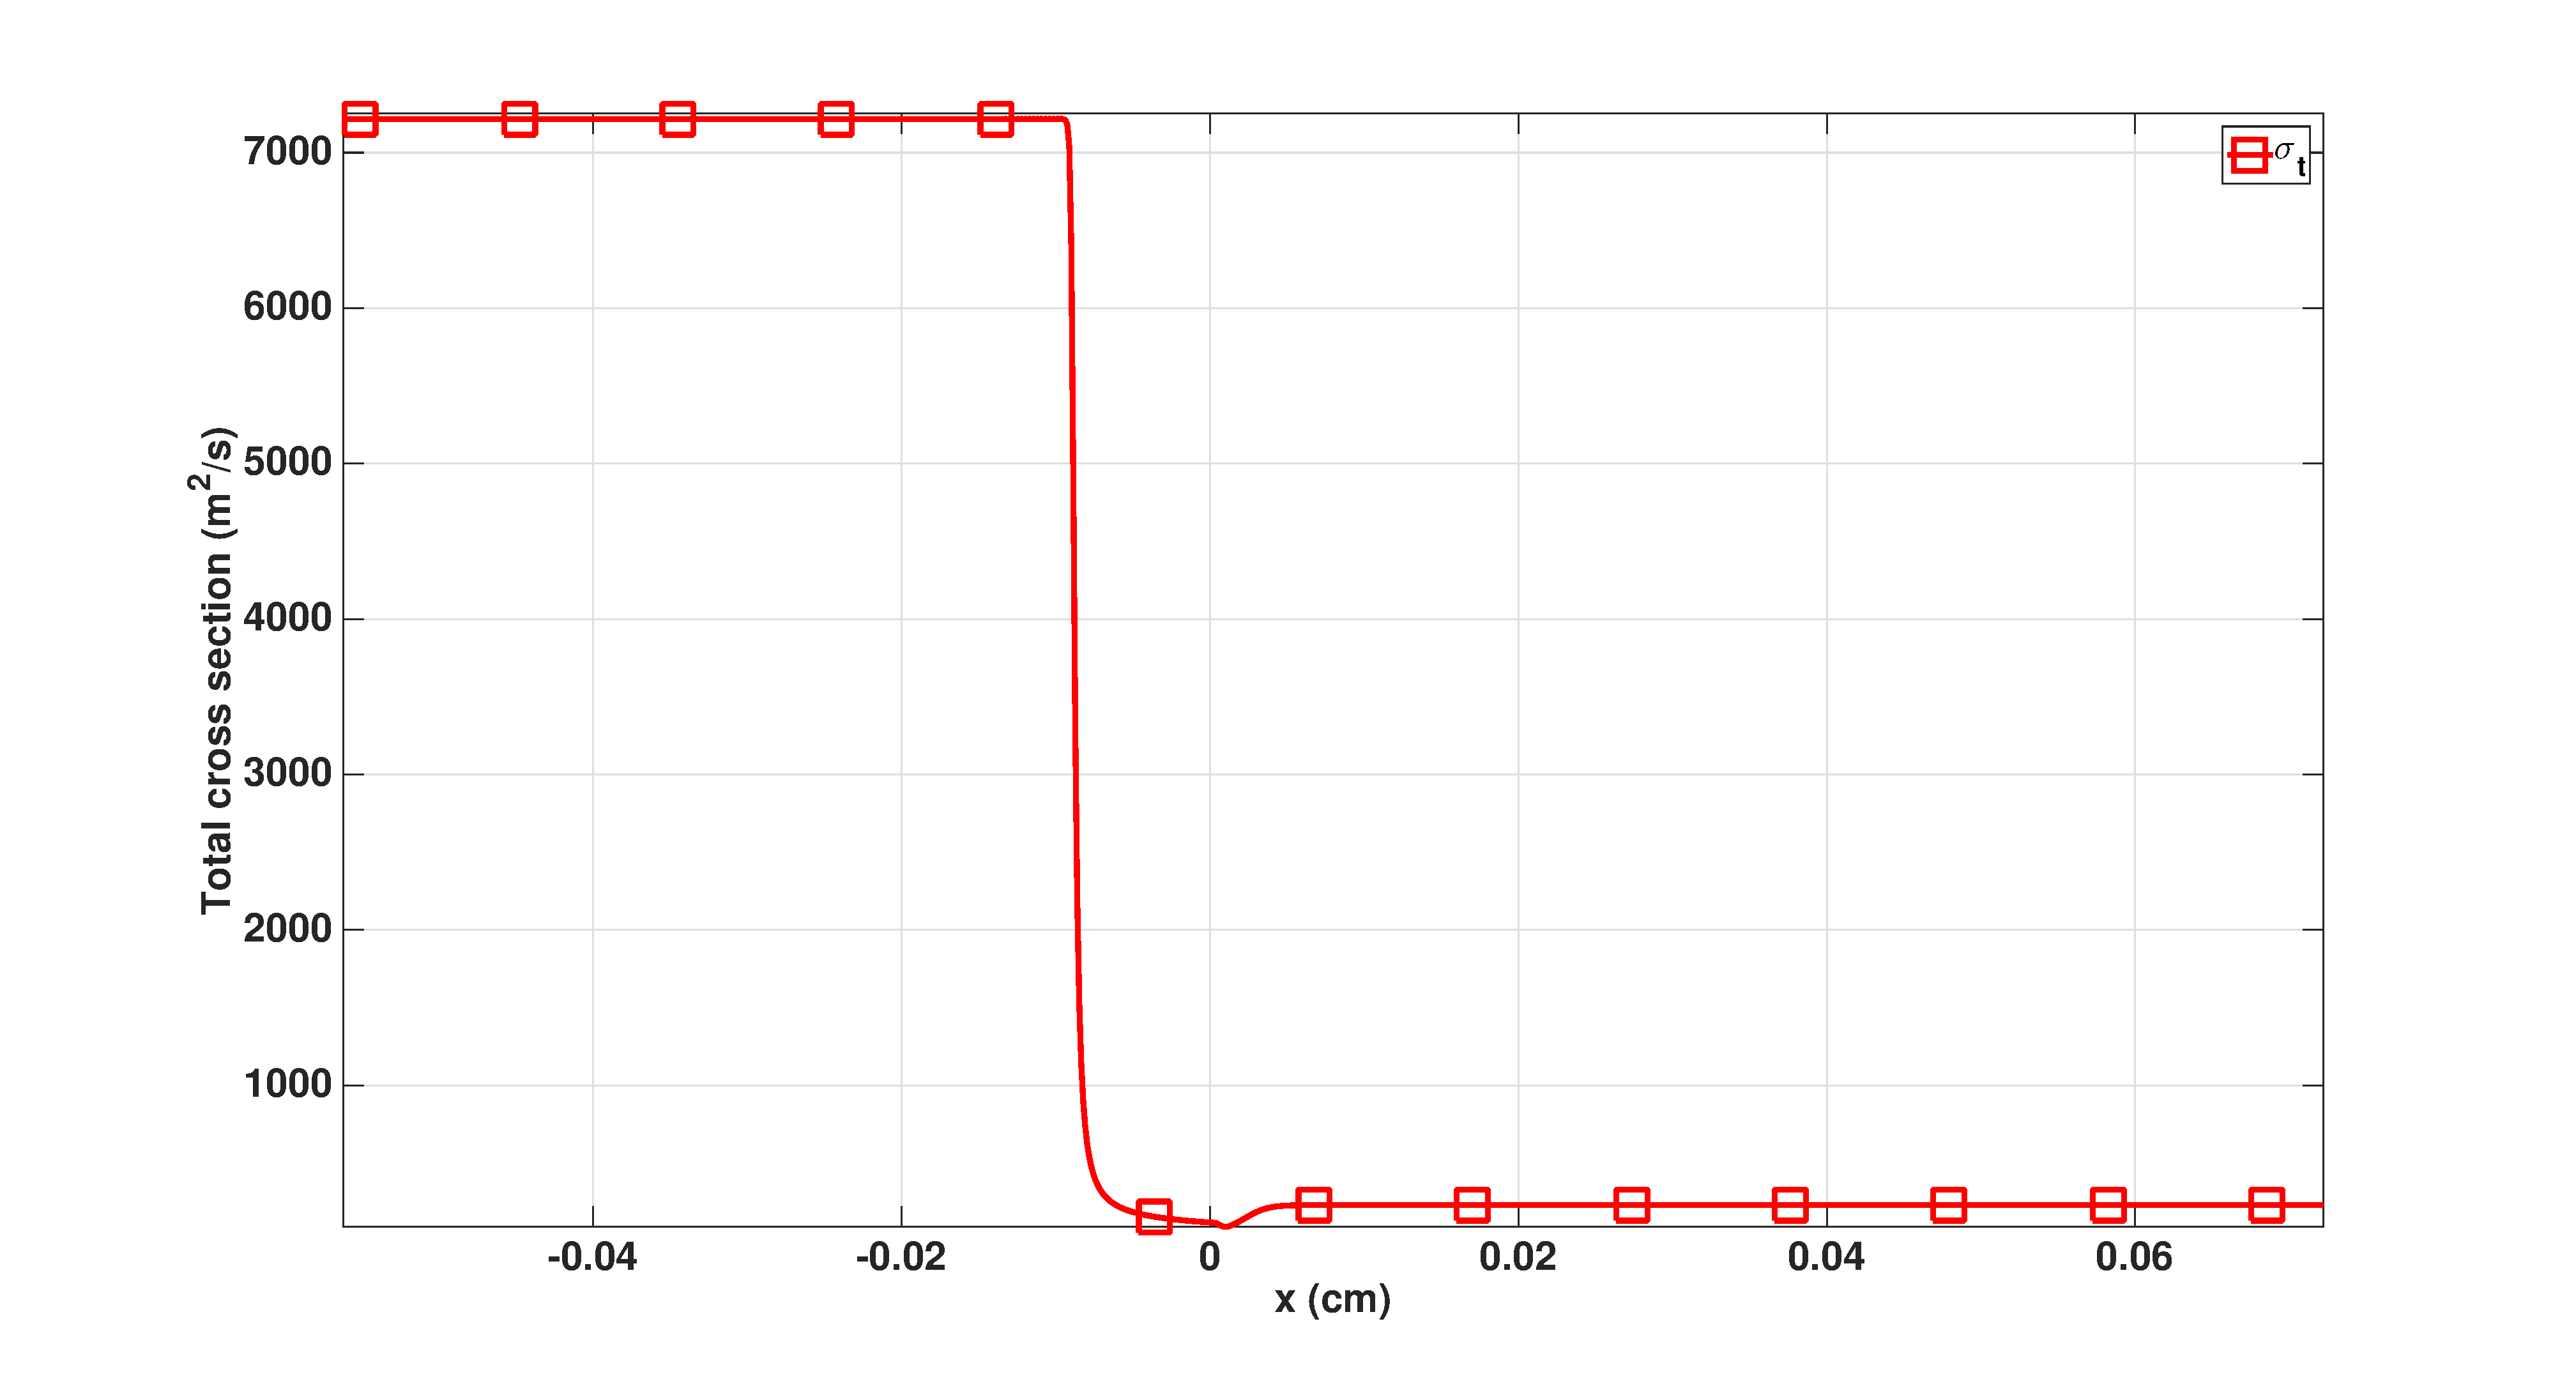
\includegraphics[width=\textwidth]{figures/dpt-xs/mach_3_nel_1000_total_cross_section.eps}
    \caption{Steady-state solution of the total opacity $\sigma_t$ for the Mach 3 shock test.}\label{fig:mach-3-dpt-xs-xs}
\end{figure}
%
\begin{figure}[H]
    \centering
    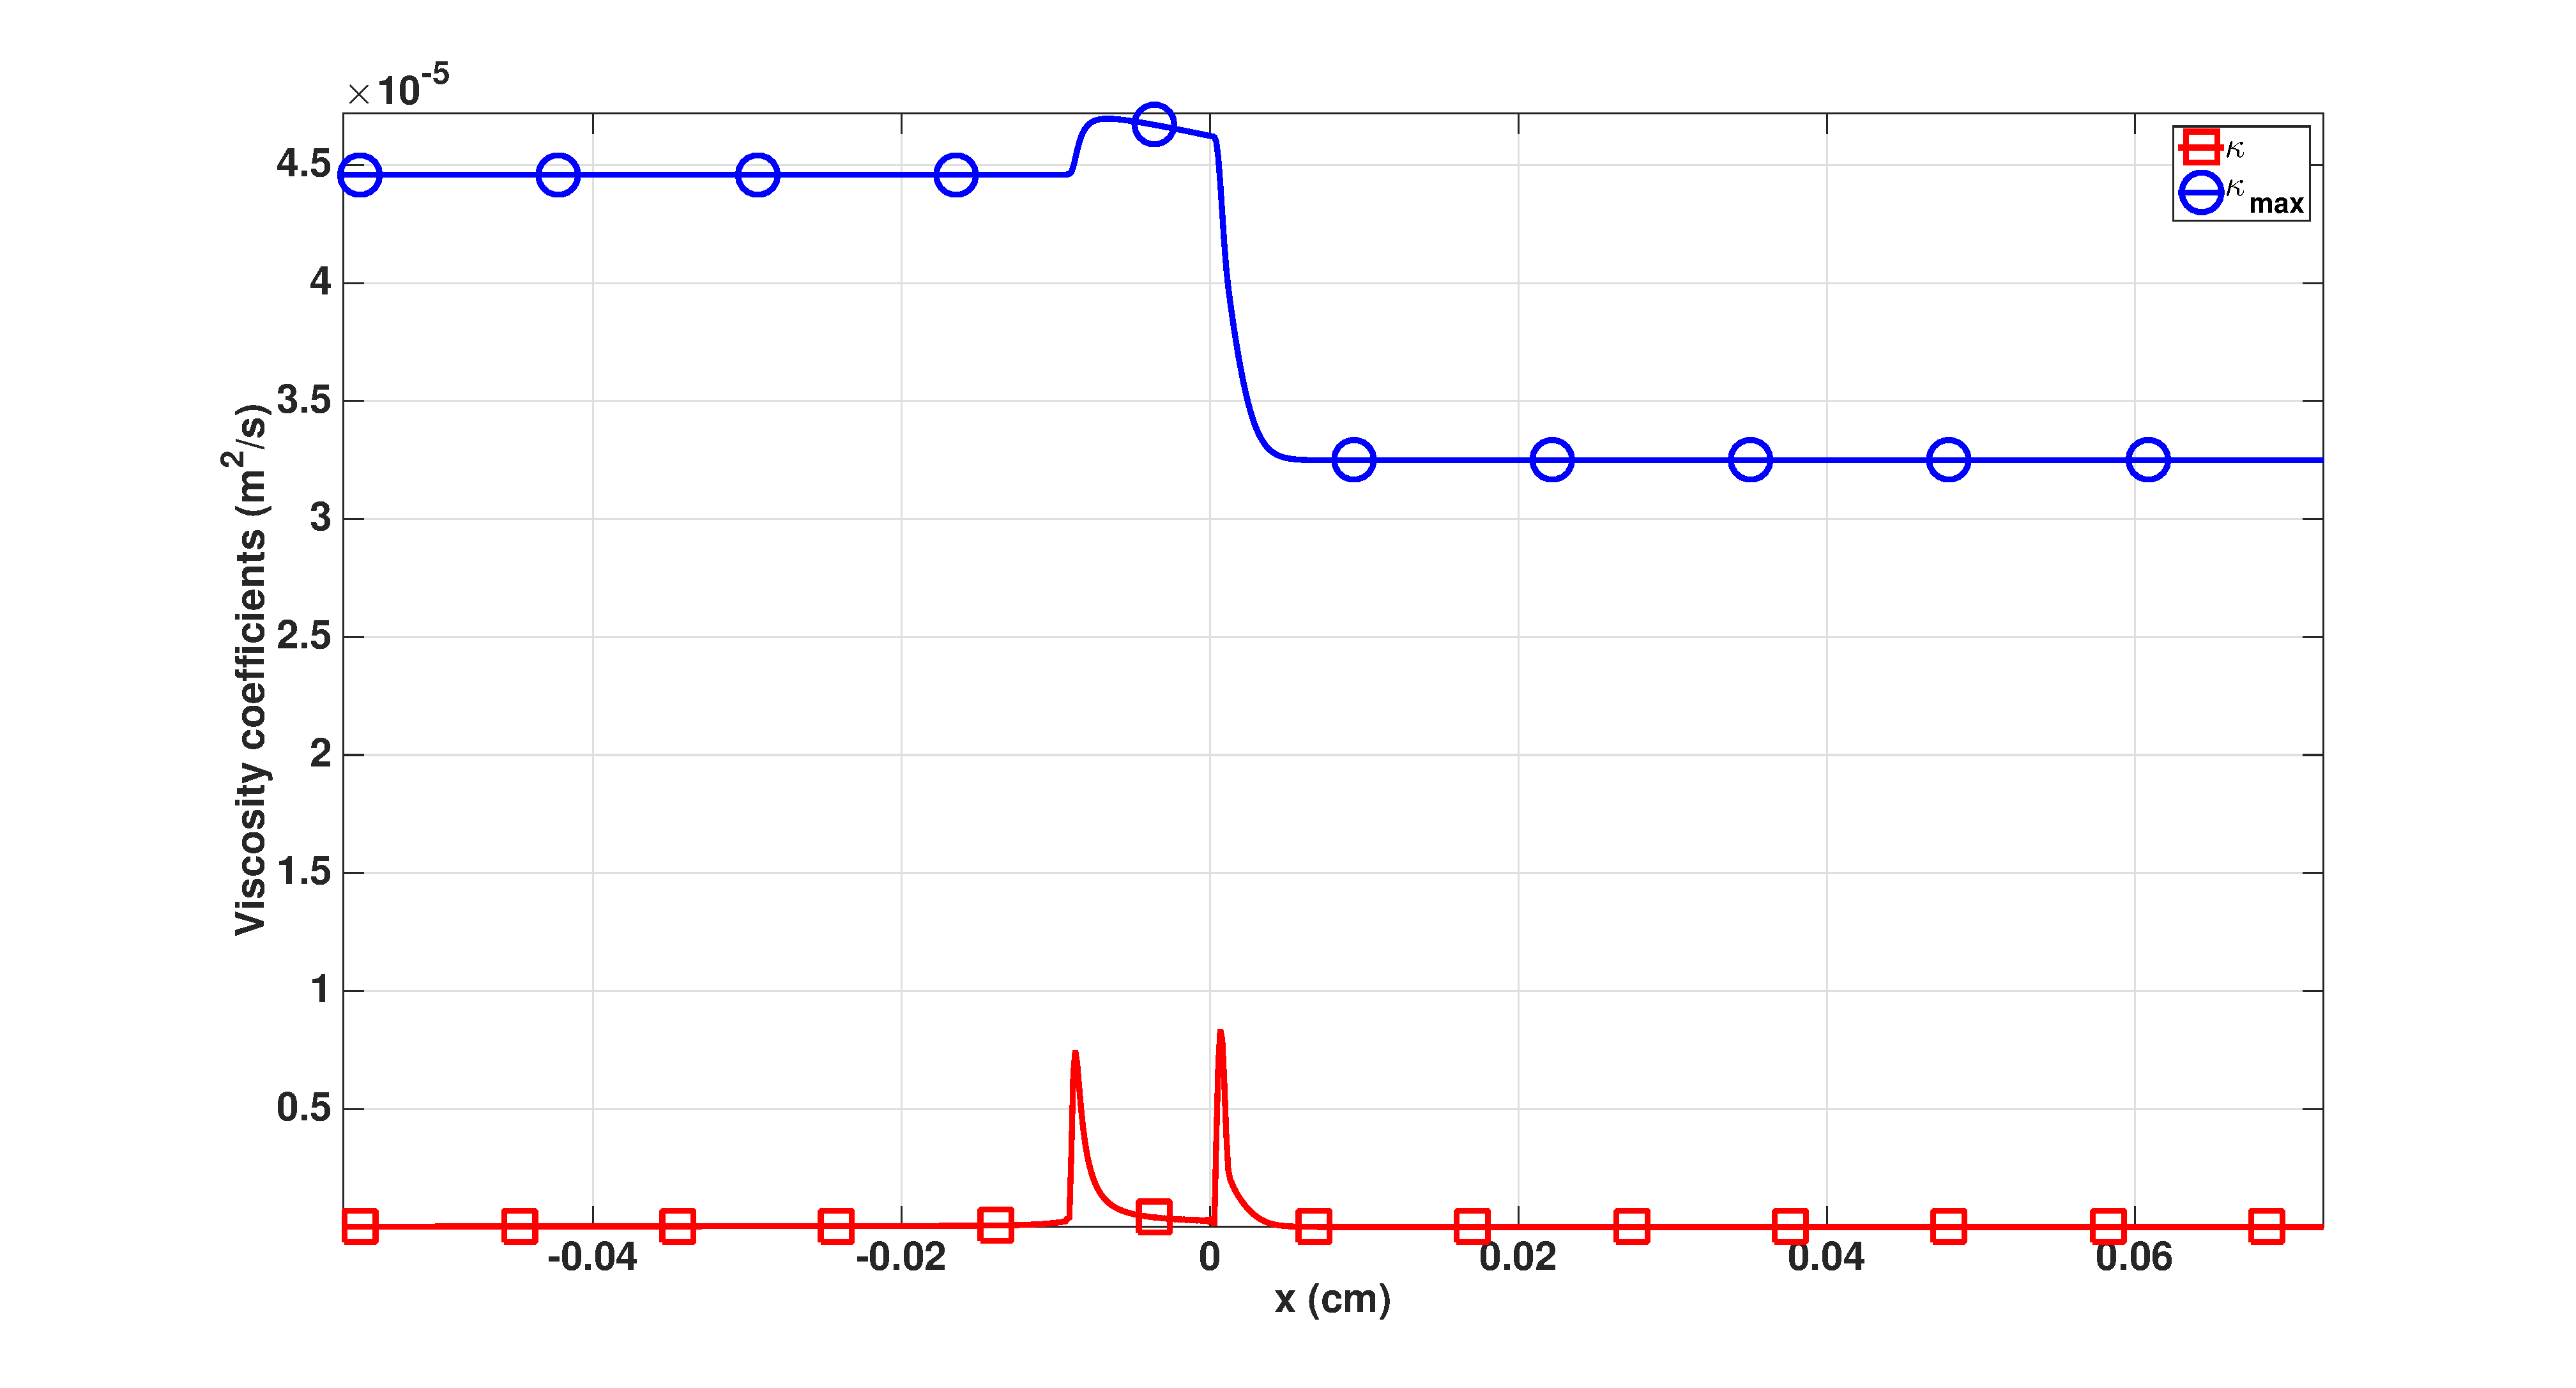
\includegraphics[width=\textwidth]{figures/dpt-xs/mach_3_nel_1000_viscosity.eps}
    \caption{Steady-state solution of the artificial viscosity coefficients for the Mach 3 shock test.}\label{fig:mach-3-dpt-xs-visc}
\end{figure}
%
%------------------------------------------------------------------
%------------------------------------------------------------------
\section{Conclusions and future work}
%------------------------------------------------------------------
%------------------------------------------------------------------
%\section{Introduction}
%\label{sec:section1}
%%%%%%%%%%%%%%%%%%%%%%%%%%%%%%%%%%%%%%%%%%%%%%%%%%%%%%%%%%%%%%
%%%%%%%%%%%%%%%%%%%%%%%%%%%%%%%%%%%%%%%%%%%%%%%%%%%%%%%%%%%%%%
%\tcr{the paper will not have the numerical results in it, so some of this introduction has to change. for example, work on rieman solvers, Edwards, may not be pertinent anymore.}
%
%Solving the radiation hydrodynamic equations is a difficult task for multiple reasons. First, the characteristic time scales between the radiation and hydrodynamics are different by several orders of magnitude which often requires the radiation part to be solved implicitly to ensure stability. Second, as with any wave-dominated problems, high resolution schemes are needed to accurately resolve shocks. Third, high-order accuracy in time and space is challenging to achieve but some recent works provide examples of such results when solving either the Euler equations \cite{Hussaini, jlg1, jlg2, Leveque} or the radiation equation \cite{nse_ragusa_wang,jcp_ragusa_wang}. 
%
%Substantial research efforts have focused on Riemann solvers for both the radiation and hydrodynamic equations. Balsara \cite{Balsara} developed a Riemann solver for the Radiation-Hydrodynamic equations by considering the frozen approximation that decouples the two physics components. However, such an approach may be questionable in the equilibrium diffusion limit. In this case, the coupling terms drive the physics and have to be accounted for. A \emph{generalized Riemann solver} that accounts exactly for the relaxation terms was developed in \cite{LowrieMorelHittinger}. Another approach assumes the strong equilibrium diffusion limit (or frozen in limit) in which radiation diffusion is negligible and the radiation simply advects at the material velocity \cite{Woodward}. In this limit, the radiation hydrodynamics equation can be expressed in the form of the Euler equations with a radiation-modified equation of state (REOS). 
%%Any solution technique for the Euler equations may be applied to these equations. Thus, one may develop approximate Riemann solvers for these equations and applied them in a more general context. 
%
%Edwards and al. \cite{EdwardsMorelLowrie} proposed a two-stage semi-implicit IMEX scheme to solve the Radiation-Hydrodynamic equations. A Riemann solver along with a flux limiter is used to resolve shocks and other waves. Their results show good agreement with semi-analytical solutions. 
%
%\tcr{check for redundancies in text below}
%In this article we propose to solve the non-equilibrium Grey Radiation-Hydrodynamics (GRH) equations by stabilizing the numerical discretization using \emph{the Entropy Viscosity Method} (EVM). This EVM, developed by Guermond et al. for hyperbolic systems of equations \cite{jlg1, jlg2}, consists in adding appropriate dissipative terms to the governing equations.  The artificial viscosity coefficient in these terms is modulated by the local entropy production. These dissipative terms are devised to stabilize the numerical scheme and to remove the non-physical oscillations appearing at the shock locations. Since entropy production is peaked in shocks \cite{Toro}, the  viscosity coefficient in the EVM is set proportional to the entropy production \tcb{that is computed on the fly}. In doing so, shocks can be detected and tracked and an adequate amount of viscosity is added locally to stabilize the numerical scheme. \tcb{TO REMOVE: The entropy production is computed on the fly, by evaluating the entropy residual. This residual is strongly peaked in shocks and small elsewhere.} 
%The entropy viscosity method was shown to achieve high-order accuracy away from the shock regions, was successfully applied to non-linear hyperbolic equations using various discretization methods (finite volume, continuous and discontinuous finite elements, spectral method) and yielded high-order accuracy on non-uniform meshes and complex geometries \cite{jlg2, valentin}. Because of the similarity between Euler equations and the radiation-hydrodynamic equations, it is conjectured that the entropy viscosity method may be a good candidate for resolving shocks occurring in radiation-hydrodynamic phenomena.
%
%The 1-D non-equilibrium Grey Radiation-Hydrodynamic equations are recalled in \eqts{eq:GRH}:
%\begin{subequations}
%\label{eq:GRH}
%%
%\begin{equation}
%\label{eq:GRHmass}
%\partial_t \left( \rho \right) + \partial_x\left( \rho u \right) = 0 
%\end{equation}
%%
%\begin{equation}
%\label{eq:GRHmom}
%\partial_t \left( \rho u\right) + \partial_x \left(\rho u^2 + P + \frac{\epsilon}{3} \right) = 0 
%\end{equation}
%%
%\begin{equation}
%\label{eq:GRHenerg}
%\partial_t \left( \rho E\right) + \partial_x \left[ u \left( \rho E + P \right) \right] = -\frac{u}{3} \partial_x \epsilon - \sigma_a c \left( a T^4 - \epsilon \right) 
%\end{equation}
%%
%\begin{equation}
%\label{eq:GRHrad}
%\partial_t \epsilon + \frac{4}{3} \partial_x \left( u \epsilon \right) = \frac{u}{3} \partial_x \epsilon + \partial_x \left( \frac{c}{3 \sigma_t} \partial_x \epsilon \right) + \sigma_a c \left( a T^4 - \epsilon \right)
%\end{equation}
%\end{subequations}
%where $\rho$, $u$, $E$, $\epsilon$, $P$ and $T$ are the material density, material velocity, material specific total energy, radiation energy density, material pressure and temperature, respectively. The total and absorption opacities, $\sigma_t$ and $\sigma_a$, are either constant or are expressed as a function of material density and temperature. The variables $a$ and $c$ are the radiation constant and the speed of light, respectively. The symbols $\partial_t$ and $\partial_x$ denote the temporal and spatial partial derivatives, respectively. 
%The material temperature and pressure are computed with the ideal gas equation of state (IGEOS): 
%$ P = (\gamma-1) C_v \rho T$ and $e = C_v T$,
%where  $e = E - 0.5 u^2$ is the specific internal energy. The heat capacity $C_v$ and the heat ratio coefficient $\gamma$ are assumed constant. 
%
%%The objective of this paper is to extend the entropy-based viscosity method to the Grey non-equilibrium Radiation-Hydrodynamic equations. 
%The approach followed in this paper is similar to those of \cite{Balsara, LowrieMorel} where the relaxation and diffusion terms in the radiation and material energy equations are omitted in order to analyze only the hyperbolic parts of \eqt{eq:GRH}. 
%%Then, an entropy equation is derived and used to obtain the functional forms of the viscous stabilization terms. Definitions for the viscosity coefficients are provided. 
%
%This paper is organized as follows. In \sect{sec:entropy-visc-meth}, the entropy viscosity method is extended to the non-equilibrium Grey Radiation-Hydrodynamic equations. Details regarding the derivation of the adequate dissipative terms and definitions for the new viscosity coefficients are provided. Spatial and temporal discretization schemes are discussed in \sect{sec:num-scheme} along with the solution algorithm employed to solve the discretized equations. Numerical results are presented in \sect{sec:num-res} where the second-order accuracy of the scheme is demonstrated in both the equilibrium-diffusion and streaming limits, using the method of manufactured solutions. Then, several numerical test cases, taken from the published literature \cite{LowrieEdwards}, are provided; in these simulations, the Mach number varies from $1.05$ to $50$. Conclusions are presented in \sect{sec:ccl}.
%
%%%%%%%%%%%%%%%%%%%%%%%%%%%%%%%%%%%%%%%%%%%%%%%%%%%%%%%%%%%%%%
%%%%%%%%%%%%%%%%%%%%%%%%%%%%%%%%%%%%%%%%%%%%%%%%%%%%%%%%%%%%%%
%\section{The entropy-based viscosity method applied to the Radiation-Hydrodynamic equations}
%\label{sec:entropy-visc-meth}
%%%%%%%%%%%%%%%%%%%%%%%%%%%%%%%%%%%%%%%%%%%%%%%%%%%%%%%%%%%%%%
%%%%%%%%%%%%%%%%%%%%%%%%%%%%%%%%%%%%%%%%%%%%%%%%%%%%%%%%%%%%%%
%
%In this section, we extend the entropy viscosity method \cite{jlg1, jlg2, valentin} to the Radiation-Hydrodynamic equations in a staged process. First, the reader is guided through the main steps that lead to the derivation of the viscous regularization based on the entropy minimum principle \cite{entropy}. Then, an asymptotic study is performed for the regularized GRH equations, i.e., with viscous dissipative terms present; we show that the equilibrium-diffusion limit is preserved for the regularized GRH equations. The frozen-in limit is also investigated and an equivalence is shown between the results presented in this paper and previously obtained results (for instance, the ones in \cite{LowrieMorel}). Finally, a definition for the entropy viscosity coefficient is presented along with the viscous regularization of the GRH equations.
% 
%%%%%%%%%%%%%%%%%%%%%%%%%%%%%%%%%%%%%%%%%%%%%%%%%%
%\subsection{Derivation of a viscous regularization for the non-equilibrium Grey Radiation-Hydrodynamic equations}\label{sec:visc-reg}
%%%%%%%%%%%%%%%%%%%%%%%%%%%%%%%%%%%%%%%%%%%%%%%%%%
%
%We recall that the entropy viscosity method was developed for hyperbolic system of equations. However, the Radiation-Hydrodynamic equations are not strictly hyperbolic but several numerical techniques are based on the characteristics of their hyperbolic parts \cite{Balsara, LowrieMorel}. Following the same rationale, we omit the relaxation and the diffusion terms in the radiation and material energy equations, \eqt{eq:GRHrad} and \eqt{eq:GRHenerg}; this yields the following hyperbolic system:
%\begin{subequations}
%\label{eq:GRH_hyperbolic}
%\begin{equation}
%\partial_t \left( \rho \right) + \partial_x\left( \rho u \right) = 0 
%\end{equation}
%%
%\begin{equation}
%\partial_t \left( \rho u\right) + \partial_x \left(\rho u^2 + P + \frac{\epsilon}{3} \right) = 0 
%\end{equation}
%%
%\begin{equation}
%\partial_t \left( \rho E\right) + \partial_x \left[ u \left( \rho E + P \right) \right] +\frac{u}{3} \partial_x \epsilon = 0
%\end{equation}
%%
%\begin{equation}
%\partial_t \epsilon + \frac{4}{3} \partial_x \left( u \epsilon \right) - \frac{u}{3} \partial_x \epsilon = 0
%\end{equation}
%\end{subequations}
%%
%The eigenvalues of the system of equations, \eqts{eq:GRH_hyperbolic}, are: 
%\begin{equation}
%\label{eq:eigenvalues_hyperbolicGRH}
%\lambda_1 = u-c_m \text{, } \lambda_{2,3} = u \text{ and } \lambda_4 = u+c_m ,
%\end{equation}
%%
%where $c_m$ is a radiation-modified material speed of sound:
%%
%\begin{equation}
%\label{eq:soundspeed}
%c_m^2 = \underbrace{P_{\rho} + \frac{P}{\rho^2}P_e}_{c_{Euler}^2} + \underbrace{\frac{4 \epsilon}{9\rho}}_{c^2_{rad}} 
%= c_{Euler}^2 + c^2_{rad} \,,
%\end{equation}
%%
%where $P_x$ is the standard shorthand notation for $\partial_x P$, $c^2_{Euler}$ denotes the speed of sound when considering only Euler equations, and $c^2_{rad}$ is the radiation contribution to the sound speed $c_m^2$. The eigenvalues given in \eqt{eq:eigenvalues_hyperbolicGRH} are unconditionally real as long as the chosen equation of state ensures a real-valued material speed of sound $c_{Euler}$. 
%Because the system given in \eqts{eq:GRH_hyperbolic} is hyperbolic, one can assume the existence of an entropy function $s$ that depends upon the internal energy $e$, the density $\rho$, and the radiation energy density $\epsilon$ (three primitive variables)  \cite{Lax}. After some algebra, given in \app{app:appendixA}, an equation satisfied by the entropy $s$ is obtained:
%\begin{equation}
%\label{eq:entropy_equation}
%\rho \frac{Ds}{Dt} = \rho \left( \partial_t s + u \partial_x s \right) \geq 0 \ ,
%\end{equation}
%where $\frac{D \cdot}{Dt}$ denotes the total or material derivative ($\frac{Ds}{Dt} = 0$  for smooth solutions). \eqt{eq:entropy_equation} is often referred as the entropy residual and is used to prove the entropy minimum principle \cite{entropy}. 
%
%Because the solutions of \eqts{eq:GRH_hyperbolic} can develop shocks, dissipative terms are added to each equation to prevent oscillatory behaviors in the numerical solution. When adding dissipative terms in \eqts{eq:GRH_hyperbolic}, the entropy residual equation is modified and some additional terms will appear in the right-hand side of \eqt{eq:entropy_equation}. The sign of these additional terms needs to be studied for the entropy minimum principle to hold. As such, the entropy minimum principle is invoked to guide in the derivation of appropriate expressions for each of the dissipative terms. Deriving the final expressions for the dissipative terms requires a few algebraic manipulations and only the final result and the key assumptions are stated here. The reader is referred to \app{app:appendixA} for the details of the derivation. The hyperbolic portion of the GRH system of equations \emph{with dissipative terms present} is as follows:
%\begin{subequations}
%\label{eq:regularized_hyperbolic_GRH}
%\begin{equation}
%\partial_t \left( \rho \right) + \partial_x\left( \rho u \right) = \partial_x \left( \kappa \partial_x \rho \right) 
%\end{equation}
%%
%\begin{equation}
%\partial_t \left( \rho u\right) + \partial_x \left(\rho u^2 + P + \frac{\epsilon}{3} \right) = \partial_x \left( \kappa \partial_x \rho u \right) 
%\end{equation}
%%
%\begin{equation}
%\partial_t \left( \rho E\right) + \partial_x \left[ u \left( \rho E + P \right) \right] + \frac{u}{3} \partial_x \epsilon = \partial_x \left( \kappa \partial_x(\rho E) \right)
%\end{equation}
%%
%\begin{equation}
%\partial_t \epsilon + \frac{4}{3} \partial_x \left( u \epsilon \right) - \frac{u}{3} \partial_x \epsilon = \partial_x \left( \kappa \partial_x \epsilon \right)
%\end{equation}
%\end{subequations}
%%
%where $\kappa$ is a positive and locally defined viscosity coefficient. The following conditions were assumed to hold:
%\begin{subequations}
%\label{eq:visc_reg_assumptions}
%\begin{equation}
%P \frac{\partial s}{\partial e} + \rho^2 \frac{\partial s}{\partial \rho} + \frac{4}{3} \rho \epsilon \frac{\partial s}{\partial \epsilon} = 0 \,,
%\end{equation}
%%
%where the functional form of the entropy is
%%
%\begin{equation}\label{eq:ent_equ}
%s( \rho, e, \epsilon) = s_{Euler}(\rho, e) + s_{rad}(\rho, \epsilon) = s_{Euler}(\rho, e)+ \frac{\beta}{\rho} \epsilon^\frac{3}{4} \,.
%\end{equation}
%%\tcb{We need to keep the form $s( \rho, e, \epsilon) = s_{Euler}(\rho, e) + \frac{\rho^{(0)}}{\rho }s_{rad}(\epsilon)$, otherwise the non-diagonal terms of the last row and column of the $3 \times 3$ matrix do not zero out, and we have to be consistent with the appendix.}
%\end{subequations}
%%
%The entropy function obtained is the sum of (i) $s_{Euler}(\rho, e)$, the entropy function obtained when considering only the Euler equations (i.e., \eqts{eq:GRH_hyperbolic} with no radiation terms) and (ii) $s_{rad}(\rho,\epsilon)=\tfrac{\beta}{\rho} \epsilon^\frac{3}{4}$, the radiation contribution to the entropy. 
%$s_{Euler}(\rho, e)$ is concave with respect to the internal energy $e$ and the specific volume $1/\rho$ and is defined through the entropy relation $Tds_{Euler} = de + P d \rho^{-1}$ given by the second law of thermodynamics. 
%$s_{rad}(\rho,\epsilon)$ is concave with respect to the radiation energy density $\epsilon$. Its functional form of is derived later, in \sect{sect:ent-asym-limit}; \tcr{I believe this is the wrong section, the next one maybe?} \tcb{I fixed it} $\beta$ is a constant. 
%The entropy $s(\rho,e,\epsilon)$ can also be obtained through a relation analogous to the second law of thermodynamics, as explained next. Starting from $Tds$ and using the expression of the entropy given in \eqt{eq:ent_equ}, a radiation-modified entropy relation is obtained:
%%
%\begin{equation}\label{eq:ent_relation}
%Tds = d\hat{e} + \left[ d\hat{P} + \epsilon \left( \frac{T \beta}{\epsilon^\frac{1}{4}} -\frac{4}{3} \right) \right] d \rho^{-1} + \rho^{-1}\left( \frac{3 T \beta}{4 \epsilon^\frac{1}{4}} -1 \right) d \epsilon
%\end{equation}
%%
%where $\hat{e}$ and $\hat{P}$ are the radiation-modified internal energy and pressure, respectively, and are defined as follows:
%%
%\begin{equation}\label{eq:rad_mod_var}
%\hat{e} = e + \frac{\epsilon}{\rho} \ \text{and} \ \hat{P} = P + \frac{\epsilon}{3} \,.
%\end{equation}
%%
%In Section \ref{sect:ent-asym-limit}, we will draw an equivalence with the above expression, valid for any regime, and previously published expressions valid in the Equilibrium-Diffusion Limit (EDL).
%
%%%%%%%%%%%%%%%%%%%%%%%%%%%%%%%%%%%%%%%%%%%%%%%%%%
%\subsection{The Equilibrium-Diffusion Limit (EDL)}\label{sect:equ-diff}
%%%%%%%%%%%%%%%%%%%%%%%%%%%%%%%%%%%%%%%%%%%%%%%%%%
%%
%Here, we carry out of an asymptotic limit for the (non-equilibrium) Grey Radiation-Hydrodynamic equations with viscous regularization present (i.e., starting from \eqts{eq:equation-visc-reg}) and investigate whether we recover the correct asymptotic equations. By correct asymptotic equations, we mean the equilibrium diffusion limit equations \emph{with} viscous regularization present. Furthermore, we will call the dissipative terms well-scaled in that limit if they 
%do not depend upon the scaling parameter.
%% \tcr{after the asymptotic analysis has been carried out}, should 
%Note that, even in the equilibrium-diffusion limit, the radiation hydrodynamic equations can develop shocks and thus require adequate stabilization.
%We compare the asymptotic results against the equilibrium-diffusion limit Radiation-Hydrodynamic equations which can be found in Section 4 of Reference \cite{LowrieMorel}, for instance. 
%%
%The full GRH equations \emph{with} the viscous regularization derived in \sect{sec:visc-reg} are as follows:
%%
%\begin{subequations}
%\label{eq:equation-visc-reg}
%\begin{equation}
%\partial_t \left( \rho \right) + \partial_x\left( \rho u \right) = \partial_x \left( \kappa \partial_x \rho \right) 
%\end{equation}
%%
%\begin{equation}
%\partial_t \left( \rho u\right) + \partial_x \left(\rho u^2 + P + \frac{\epsilon}{3} \right) = \partial_x \left( \kappa \partial_x (\rho u) \right) 
%\end{equation}
%%
%\begin{equation}
%\partial_t \left( \rho E\right) + \partial_x \left[ u \left( \rho E + P \right) \right] = -\frac{u}{3} \partial_x \epsilon - \sigma_a c \left( a T^4 - \epsilon \right) + \partial_x \left( \kappa \partial_x (\rho E)\right)
%\end{equation}
%%
%\begin{equation}
%\partial_t \epsilon + \frac{4}{3} \partial_x \left( u \epsilon \right) = \frac{u}{3} \partial_x \epsilon + \partial_x \left( \frac{c}{3 \sigma_t} \partial_x \epsilon \right) + \sigma_a c \left( a T^4 - \epsilon \right) + \partial_x \left( \kappa \partial_x \epsilon \right)
%\end{equation}
%\end{subequations}
%%
%
%To derive the scaled version of \eqts{eq:equation-visc-reg}, we consider the following non-dimensionalization:
%%
%\begin{equation}
%\label{eq:norm_param}
%\begin{array}{llll}
%\rho'   = \frac{\rho}{\rho_\infty}           , & 
%u'      = \frac{u}{c_{m,\infty}}                 , & 
%P'      = \frac{P}{\rho_\infty c^2_{m,\infty}}   , & 
%\epsilon'      = \frac{\epsilon}{a T_\infty^4 }              , \\
%E'      = \frac{E}{c^2_{m,\infty} }              , & 
%\sigma_t'      = \frac{\sigma_t}{\sigma_{t,\infty} }              , & 
%\sigma_a'      = \frac{\sigma_a}{\sigma_{a,\infty} }              , & 
%T'      = \frac{T}{T_\infty }              , \\
%x' = \frac{x}{L_\infty}                      , & 
%t' = \frac{t}{L_\infty / c_{m,\infty}}       , &  
%\kappa' = \frac{\kappa}{\kappa_\infty}       ,
%\end{array}
%\end{equation}
%%
%where  the subscript $\infty$ denote the far-field quantities and the superscript $'$ 
%stands for the non-dimensional variables. The far-field reference quantities are chosen such that the 
%dimensionless quantities are of order one. Note that $\sigma_a$ will be expressed as $\sigma_t - \sigma_s$.  Using the scaled variables introduced in \eqt{eq:norm_param}, the non-dimensionalized equations are as follows:
%%
%\begin{subequations}
%\label{eq:equation-visc-reg-scaled}
%\begin{equation}
%\partial_{t'} \left( \rho' \right) + \partial_{x'}\left( \rho' u' \right) = \Pe \partial_x \left( \kappa' \partial_{x'} \rho' \right) 
%\end{equation}
%%
%\begin{equation}
%\partial_{t'} \left( \rho' u'\right) + \partial_{x'} \left(\rho u^{2'} + P' + \Re \frac{\epsilon'}{3} \right) = \Pe \partial_{x'} \left( \kappa' \partial_{x'} (\rho' u') \right) 
%\end{equation}
%%
%\begin{multline}
%\partial_{t'} \left( \rho' E'\right) + \partial_{x'} \left[ u' \left( \rho' E' + P' \right) \right] 
%= 
%-
%\Re \frac{u'}{3} \partial_{x'} \epsilon' 
%\\ 
%- 
%\Re \Us^{-1} \Ls \left( \sigma_t' - \Lsi \sigma_s' \right)  \left(T^{\prime,4} - \epsilon' \right) 
%+ 
%\Pe \partial_{x'} \left( \kappa' \partial_{x'} (\rho' E')\right)  
%\end{multline}
%%
%\begin{multline}
%\partial_{t'} \epsilon' + \frac{4}{3} \partial_{x'} \left( u' \epsilon' \right) 
%= \frac{u'}{3} \partial_{x'} \epsilon' 
%+ 
%\Ls^{-1} \Us^{-1} \partial_{x'} \left( \frac{1}{3 \sigma_t'} \partial_{x'} \epsilon' \right) 
%\\ + 
%\Us^{-1} \Ls \left( \sigma_t' - \Lsi \sigma_s' \right) \left( T^{\prime,4} - \epsilon' \right) 
%+ 
%\Pe \partial_{x'} \left( \kappa' \partial_{x'} \epsilon' \right)
%\end{multline}
%\end{subequations}
%%
%where we introduced the following non-dimensional parameters
%%
%\begin{multline}\label{eq:scaled-nb}
%\Ls = L_\infty \sigma_{t,\infty} \ , 
%\Lsi = \frac{\sigma_{s,\infty}}{\sigma_{t,\infty}} \ , \\
%\Us = \frac{c_{m,\infty}}{c} \ ,   
%\Re = \frac{a T^4_\infty}{\rho_\infty c^2_{m,\infty} } 
%\text{ and } \Pe = \frac{\kappa_\infty}{c_{m,\infty} L_\infty} \ .
%\end{multline}
%%
%The relativistic effects are measured by the parameter $\Us$ that represents the ratio of the material speed to the speed of light; it is scaled as  $O(\varepsilon)$, where $\varepsilon \to 0$ in the equilibrium diffusion limit (EDL).
%%
%The parameter $\Ls$ denotes the ratio of the characteristic spatial scalelength of the radiation-hydrodynamic solution to the radiation mean-free-path; it scales as $O(\varepsilon^{-1})$ in the EDL in order to have an optically thick configuration. 
%%
%The parameter $\Lsi$ represents the ratio of the total mean-free-path to the scattering mean-free-path and scales as $O(\varepsilon)$. 
%%
%$\Re$ is a measure of the ratio of the radiation energy to the material energy; it is scaled as $O(1)$. 
%%
%Finally, the P\'eclet number $\Pe$ measures the ratio of the viscous term to the advection term. When it is scaled as $O(1)$, the equilibrium-diffusion equations with viscous stabilization are recovered. 
%%
%The adequate scaling of the P\'eclet number can be inferred from the scaled continuity equation, for instance. If one assumes that $\Pe$ scales as $O(\varepsilon)$, then the leading-order continuity equation does not have any stabilization terms. If one assumes $\Pe = O(\varepsilon^{-1})$, completely erroneous leading-order equations are obtained. Hence, the proper scaling is $\Pe = O(1)$ in order to yield well-scaled dissipative terms. 
%
%Hereafter, we omit the superscript $'$ for the non-dimensional variables.
%Next, we assume that each variable is expanded in a power series in $\varepsilon$, e.g.,
%%
%\begin{equation}\label{eq:expansion-series}
%\varphi = \sum_i \varphi_i \varepsilon^i \ ,
%\end{equation}
%%
%where $\varphi$ denotes any given variable. By substituting the power series expansion for each variable into the non-dimensional
%radiation-hydrodynamics equations, \eqts{eq:equation-visc-reg-scaled}, we obtain a hierarchy of asymptotic equations. By collecting all terms multiplying each power of $\varepsilon$, the leading-, first- and second-order equations are obtained. The leading-order results from \eqts{eq:equation-visc-reg-scaled} are:
%%
%\begin{subequations}
%\label{eq:first-order}
%%
%\begin{equation}
%\partial_t \rho_0 + \partial_x \left( \rho u \right)_0 = \partial_x \left( \kappa \partial_x  \rho \right)_0  \ ,
%\end{equation}
%%
%\begin{equation}
%\partial_t \left( \rho u \right)_0 + \partial_x \left( \rho u^2 + P + \frac{\epsilon}{3}\right)_0 = \partial_x \left( \kappa \partial_x \left( \rho u \right) \right)_0  \ ,
%\end{equation}
%%
%\begin{equation}\label{eq:expansion-series_energy}
%\epsilon_0 = T_0^4  \ .
%\end{equation}
%%
%\end{subequations}
%%
%%
%\eqt{eq:expansion-series_energy} states that the leading order terms for the material energy and the radiation energy are identical. One can similarly show that the first-order material energy and radiation equations also yield: $\epsilon_1 = T_1^4$. The asymptotic total energy equation is obtained by taking the second-order material and radiation energy equations and summing them to cancel the second-order relaxation terms, yielding:
%%
%\begin{equation}
%\partial_x \left( \rho E^* \right)_0 + \partial_x \left[ u \left( \rho E^* + P^* \right) \right]_0 = \partial_x \left( \frac{1}{3 \sigma_t} \partial_x \epsilon \right)_0 + \partial_x \left( \kappa \partial_x \rho E^* \right)_0
%\end{equation}
%%
%where $P^* = P + \Re \frac{T^4}{3}$ and $e^* = e + \Re \frac{T^4}{\rho}$ are the radiation-modified pressure and internal energy and match the definitions given in \cite{LowrieMorel}; recall that $\Re$ is $O(1)$. The equilibrium-diffusion system of equations is obtained by taking the leading-order continuity and momentum equations, and the second-order total energy equation, i.e.,
%%
%\begin{subequations}
%\label{eq:equip-diff-equ}
%%
%\begin{equation}
%\partial_t \rho_0 + \partial_x \left( \rho u \right)_0 = \partial_x \left( \kappa \partial_x  \rho \right)_0  \ ,
%\end{equation}
%%
%\begin{equation}
%\partial_t \left( \rho u \right)_0 + \partial_x \left( \rho u^2 + P^* \right)_0 = \partial_x \left( \kappa \partial_x \left( \rho u \right) \right)_0  \ , 
%\end{equation}
%%
%\begin{equation}
%\partial_x \left( \rho E^* \right)_0 + \partial_x \left[ u \left( \rho E^* + P^* \right) \right]_0 = \partial_x \left( \frac{1}{3 \sigma_t} \partial_x T^4 \right)_0 + \partial_x \left( \kappa \partial_x \rho E^* \right)_0 \ . \end{equation}
%%
%\end{subequations}
%%
%The viscous regularization proposed in \sect{sec:visc-reg} for the non-equilibrium GRH equations conserves the equilibrium-diffusion limit and ensures the stability of the resulting \eqts{eq:equip-diff-equ} by yielding dissipative terms that scale appropriately in each equation of \eqts{eq:equip-diff-equ}. When removing the diffusion term, $\partial_x \left( \frac{1}{3 \sigma_t} \partial_x T^4 \right)_0$, \eqts{eq:equip-diff-equ} yield a hyperbolic system of equations stabilized by a parabolic regularization \cite{Parabolic} which ensures that the entropy minimum principle holds. The viscous regularization obtained here in the equilibrium-diffusion limit is the one that would have been obtained had we studied the hyperbolic parts of the equilibrium-diffusion system of equations. This proof is provided in \app{app:appendixB} where we demonstrate that the same viscous regularization can also be obtained by stabilizing the equilibrium-diffusion limit equations.
%%
%%%%%%%%%%%%%%%%%%%%%%%%%%%%%%%%%%%%%%%%%%%%%%%%%%
%\subsection{Scaling of the entropy function derived for the non-equilibrium RHD equation in the Equilibrium-Diffusion Limit}\label{sect:ent-asym-limit}
%%%%%%%%%%%%%%%%%%%%%%%%%%%%%%%%%%%%%%%%%%%%%%%%%%
%%
%We also investigate how the asymptotic limit affects the entropy function $s(\rho, e, \epsilon)$, given in \eqt{eq:visc_reg_assumptions} and derived when only considering the hyperbolic terms of the non-equilibrium grey RHD. We first derive the non-dimensionalized entropy by scaling the entropy with $\frac{c_{m,\infty}^2}{T_\infty}$, which yields:
%%
%\begin{equation}\label{eq:ent-scaled}
%s' \left( \rho', e', \epsilon' \right) = s'_{Euler} \left( \rho', e' \right)+ \Re \frac{\beta_\infty}{a\frac{1}{4}} \frac{\beta'}{\rho'} \epsilon^{\prime,3/4} \,.
%\end{equation}
%%
%Note that the non-dimensionalized $\beta'$ is equal to one since $\beta$ is a constant. $\beta_\infty$ is the reference value for $\beta$ and has the same units as $s_0 / \epsilon^\frac{3}{4}$ as shown in \app{app:appendixA}. Recalling that $\Re = O(1)$ and $T_0^4 = \epsilon_0$, the leading-order entropy term is (the superscripts are omitted for brevity):
%%\tcr{the $_0$ seem mis-placed} \tcb{ done}
%%
%\begin{equation}\label{eq:ent-scaled-2}
%s_0 \left( \rho, e \right) = s_{Euler,0}\left( \rho, e \right) + \frac{\beta_\infty}{a\frac{1}{4}} \frac{1}{\rho_0} T_0^3 \ .
%\end{equation}
%%
%We compare \eqt{eq:ent-scaled-2} against the non-dimensionalized entropy $s^*$ obtained in the equilibrium-diffusion limit with the radiation-modified Equations of State (REOS) given in Section 4 of \cite{LowrieMorel}:
%%
%\begin{equation}\label{eq:ent-reos}
%s^*(\rho,e) = s_{Euler}(\rho,e) + \frac{4T^3}{3\rho} \ .
%\end{equation}
%%
%In order to have the two entropy functions identical in the equilibrium-diffusion in limit, one simply sets $\beta_\infty = \frac{4}{3} a^\frac{1}{4}$. thus, the \emph{dimensionalized} non-equilibrium entropy function is 
%%
%\begin{equation}\label{eq:entropy}
%s \left( \rho, e, \epsilon \right) = s_{Euler}\left( \rho, e \right) + s_{rad}(\rho,\epsilon)= s_{Euler}\left( \rho, e \right) + \frac{4a^\frac{1}{4}}{3\rho} \epsilon^\frac{3}{4} \,.
%\end{equation}
%%
%%The constant $\beta$ is now fully determined and the final expression of the entropy 
%\eqt{eq:entropy} can now be used for two purposes: (i) to recast the radiation contribution to the definition of the speed of sound given in \eqt{eq:soundspeed} under the form of a partial derivative as with the definition of the speed of sound for the standard Euler equations and (ii) to derive an expression for the entropy relation (\eqt{eq:ent_relation}) in a form analogous to the second law of thermodynamics. We start with (i): Using the definition of the radiation entropy, $s_{rad}$, given in \eqt{eq:entropy}, it can be shown that:
%%
%\begin{equation}\label{eq:sp-sd-rad}
%c^2_{rad} = \frac{4 \epsilon}{9 \rho} = \left. \frac{\partial P_{rad}}{\partial \rho}\right|_{s_{rad}} \ ,
%\end{equation}
%%  
%where $P_{rad} = \frac{\epsilon}{3}$ is the radiation pressure. Using \eqt{eq:sp-sd-rad}, the speed of sound $c_m^2$ can be rewritten as follows:
%%
%\begin{equation}
%c_m^2 = c_{Euler}^2 + c_{rad}^2 = \left. \frac{\partial P}{\partial \rho} \right|_{s_{Euler}} + \left. \frac{\partial P_{rad}}{\partial \rho} \right|_{s_{rad}} \,.
%\end{equation} 
%In \cite{LowrieMorel}, Lowrie and Morel show that the radiation-modified soundspeed in the EDL can be written as
%\begin{subequations}
%\begin{equation} 
%c_m^2 = c_{Euler}^2 + \frac{4}{3}\frac{\mathbb{P} T^4}{\rho}\frac{\Gamma(2-3\Gamma) + \frac{4\mathbb{P} T^4 g}{3P}}{1+\frac{4\mathbb{P} T^4 g}{P}}
%\end{equation}
%which is maximum for $\Gamma=1/3$. In this case, Lowrie and Morel's expression becomes
%\begin{equation} \label{eq:soundspeedEDL}
%c_m^2 = c_{Euler}^2  + \frac{4}{9} \frac{\mathbb{P}T^4}{\rho} \,,
%\end{equation}
%from which we conclude that their soundspeed is less than or equal to our expression \eqt{eq:soundspeed} (the expressions are equal in the EDL).
%\end{subequations}
%
%%We now give the final expression for the entropy relation by s
%Regarding (ii), we substitute the definition of the constant $\beta = \frac{3a^\frac{1}{4}}{4}$ in \eqt{eq:ent_relation} to obtain
%%
%\begin{equation}\label{eq:ent_relation2}
%Tds = d\hat{e} + \left[ d\hat{P} + \frac{4}{3}\epsilon \mathbb{D} \right] d \rho^{-1} + \rho^{-1}\mathbb{D} \ d \epsilon \,,
%\end{equation}
%%
%where $\mathbb{D} = \left(\frac{aT^4}{\epsilon}\right)^\frac{1}{4}-1$ is a non-dimensional number that measures how close to the equilibrium-diffusion limit the problem configuration is. From \eqt{eq:expansion-series_energy}, we infer that $\mathbb{D} \to 0$ in the equilibrium-diffusion limit, which allows us to recover the entropy relationship valid in the frozen in limit and given in \cite{LowrieMorel}:
%%
%\begin{equation}
%Tds^* = de^* + P^*d \rho^{-1} \ .
%\end{equation}
%%
%Note that $e^* = \hat{e}$ and $P^* = \hat{P}$ in the equilibrium-diffusion limit.
% 
%In this section, we demonstrated that the viscous regularization derived for the hyperbolic terms of the non-equilibrium Grey Radiation-Hydrodynamic equations yields the correct asymptotic limit in the equilibrium-diffusion limit and that the leading-order  of the entropy function $s(\rho, e, \epsilon)$ tends to the EDL entropy $s^*$ given in \cite{LowrieMorel}. We were also able to recast the definition of the soundspeed in terms of partial derivatives of the material and radiation pressures.
%%
%%%%%%%%%%%%%%%%%%%%%%%%%%%%%%%%%%%%%%%%%%%%%%%%%%
%\subsection{Definition of the viscosity coefficients}
%%%%%%%%%%%%%%%%%%%%%%%%%%%%%%%%%%%%%%%%%%%%%%%%%%
%%
%Now that the dissipative terms have been obtained and shown to scale appropriately in the EDL, we define the local viscosity coefficient $\kappa(x,t)$. Following \cite{jlg1, jlg2}, we require the following to hold:
%\begin{itemize}
%\item Since the entropy residual is a measure of the entropy production, it is natural to define a viscosity coefficient proportional to the entropy residual. This will enable shock detection and shock tracking as well as provide a measure of the viscosity required to stabilize the scheme. This viscosity coefficient is referred to as the \emph{entropy viscosity coefficient} and is denoted by $\kappa_e(x,t)$.
%\item An upper bound for $\kappa$ is to be set since entropy production can be very large in shocks. For explicit time discretization, the maximum value of the viscosity coefficient is related to the Courant-Friedrichs-Lewy number (CFL). The upper bound on  $\kappa$  is defined by analogy to the standard upwind (Godunov) scheme that is known to efficiently smooth out oscillations (but is only first-order accurate). With implicit temporal integrators, the same reasoning is used even if the CFL number may not need to be strictly respected. This upper bound will be referred to as the \emph{first-order viscosity} and is denoted by $\kappa_{max}(x,t)$.  
%\item The actual viscosity coefficient $\kappa$ used in the dissipative terms of \eqt{eq:GRH_hyperbolic} is then taken to be the minimum of the above two viscosities:  $\kappa(x,t) = \min ( \kappa_e(x,t), \kappa_{max}(x,t) )$. With such a definition, the viscosity added to the system of equations will saturate to the first-order viscosity in shock regions; elsewhere, the entropy production and thus the viscosity coefficient $\kappa$ are expected to be small.
%\end{itemize}
%
%Next, we define the local first- and entropy viscosity coefficients $\kappa_{max}(x,t)$ and $\kappa_e(x,t)$, respectively. Following \cite{valentin}, the first-order viscosity definition is based on the local largest eigenvalue that is known to be $|u| + c_m$ in 1-D:
%\begin{equation}
%\label{eq:equation8}
%\kappa_{max} = \frac{h}{2} \left( |u| + c_m \right) \,,
%\end{equation}  
%where $h$ is the local grid size. This definition is derived based on the upwind scheme and a simple derivation can be found in \cite{jlg1} in the case of a scalar hyperbolic equation. Through the definition of the radiation-modified speed of sound $c_m$, both the material and radiation properties are accounted for in the definition of the first-order viscosity coefficient. Since the soundspeed of the non-equilibrium radiation hydrodynamic equation is always greater than or equal to the soundspeed of the equilibrium-diffusion equations (see previous Section, \sect{sect:ent-asym-limit}), the value used for the first-order viscosity is always large enough, whether in the equilibrium diffusion limit or not.
%
%The definition of the entropy viscosity coefficient $\kappa_e(x,t)$ is based upon the entropy residual (\eqt{eq:entropy_equation}) which is recast as a function of total pressure $\hat{P}$, density $\rho$ and soundspeed (see \app{app:appendixC} for details):
%\begin{equation}
%\label{eq:equation9}
%\tilde{D}_e(x,t) = \frac{s_e}{P_e} \underbrace{ \left( \frac{D\hat{P}}{Dt} - c_m^2 \frac{D\rho}{Dt} \right)}_\textrm{$\hat{D}_e(x,t)$} \,.
%\end{equation}
%The term $s_e$ is the inverse of the material temperature (see \app{app:appendixA}) and $P_e$ is computed from the equation of state. These two terms are positive so that the sign of the entropy residual $\tilde{D}_e(x,t)$ can be determined by simply inspecting the terms inside the parentheses, denoted by $\hat{D}_e(x,t)$. Such an expression is easier to compute than the one given in \eqt{eq:entropy_equation} which would require an analytical expression for the entropy function. Note that when deriving the non-dimensional expression of $\tilde{D}_e(x,t)$ using the reference variables of \eqt{eq:norm_param}, the adimensional entropy residual is function of the scaling parameter $\Re$ that scales as one, and thus does not depend on $\varepsilon$. In addition to the entropy residual, inter-element jumps in the pressure and density gradients, $J$, are also accounted for. By using these jump terms, one can also detect discontinuities that are not shocks, such as contact waves (there is no entropy production in a contact wave), and stabilize such waves when needed. \\
%Thus, the entropy viscosity coefficient $\kappa_e(x,t)$ is set to be proportional to $\hat{D}_e(x,t)$ and $J$ with the following form: 
%\begin{equation}
%\label{eq:equation12}
%\kappa_e(x,t) = h^2 \frac{\max (|\hat{D}_e(x,t)|, J)}{\norm_P}
%\end{equation} 
%where $J = \max_i (J(x_i,t))$, and $J(x_i,t)$ is the jump of a given quantity at cell interface $x_i$. The normalization factor $\norm_P$ (of units of pressure) is to be chosen such that the viscosity coefficient $\kappa$ (units of $m^2/s$) scale adequately in the equilibrium-diffusion limit and yields the correct asymptotic behavior. Using the definition of the viscosity coefficient given in \eqt{eq:equation12} and the scaling of \eqt{eq:norm_param}, it can be shown that:
%%
%\begin{equation}\label{eq:kappa_infty}
%\kappa_\infty = \frac{\rho_\infty c^3_{m,\infty}  L_\infty}{\norm_{P,\infty}} \ .
%\end{equation}
%%
%The scaling of the viscosity coefficient, $\kappa_\infty$, is tied to the P\'eclet number $\Pe$ defined in \eqt{eq:scaled-nb}. We demonstrated that $\Pe$ should scale as one in order to preserve the equilibrium-diffusion limit. From this, we conclude that (using the definition of the P\'eclet number) 
%%
%\begin{equation}
%\norm_{P,\infty} = \rho_\infty c^2_{m,\infty} \nonumber \ ,
%\end{equation}
%%
%Thus, the final definition for the viscosity coefficient $\kappa$ is as follows:
%\begin{equation}
%\label{eq:equation12bis}
%\kappa_e(x,t) = h^2 \frac{\max (|\hat{D}_e(x,t)|, J)}{\rho c_m^2} \ .
%\end{equation} 
%% In practice, the viscosity coefficients are only evaluated at quadrature points. 
%The jump $J$ in the definition of $\kappa(x,t)$ is piecewise-constant. Its definition is discretization-dependent and defined as follows for a continuous Galerkin FEM: 
%\begin{subequations}
%\label{eq:equation12ter}
%\begin{equation}
%J(x_i,t) = \max( J_{\rho}(x_i,t), J_{\hat{P}}(x_i,t) )
%\end{equation}
%with
%\begin{equation}
%J_{\hat{P}}(x_i,t) = |u| [[\partial_x \hat{P}]]
%\end{equation}
%and
%\begin{equation}
%J_{\rho}(x_i,t) = c_m^2 |u|  [[\partial_x \rho]] \,.
%\end{equation}
%\end{subequations}
%The symbol $[[ \cdot ]]$ denotes the jump at the cell interface.
%
%The entropy viscosity method is now well defined for the hyperbolic system given in \eqt{eq:GRH_hyperbolic} and will be used to solve for the non-equilibrium Grey Radiation-Hydrodynamic equations given in \eqt{eq:GRH}. However, one may question how the relaxation source terms, $\sigma_a c (a T^4-\epsilon)$ and the physical diffusion term, $\partial_x(D\partial_x \epsilon)$, may affect the entropy viscosity method. When applying the entropy viscosity method, the radiation energy density equation will now contain a diffusive term and a numerical dissipative term with a vanishing viscosity coefficient $\kappa$. As long as the diffusive coefficient $D=\frac{c}{3 \sigma_t}$ is larger than the viscosity coefficient $\kappa$, the numerical dissipative term should not be required. A way to ensure consistency and prevent the formation of oscillations in the frozen limit is to merge the two second-order derivative terms into one as follows:
%\begin{equation}
% \partial_x \left( \frac{c}{3 \sigma_t} \partial_x \epsilon \right) + \partial_x \left( \kappa \partial_x \epsilon \right) 
% \Longrightarrow
% \partial_x \left[ \max\left(\frac{c}{3 \sigma_t} \text{, } \kappa \right) \partial_x \epsilon \right]
%\end{equation}
%\tcb{TO REMOVE: Thus, as long as the artificial viscosity coefficient $\kappa$ is locally smaller that the physical diffusive coefficient $D=\frac{c}{3 \sigma_t}$, no artificial viscosity is required to ensure stability of the numerical scheme. As the diffusive coefficient $D$ goes to zero, shocks can form in the radiation energy density profile and will require a certain amount of viscosity in order to prevent oscillations from appearing.}
%\tcr{text seems redundant here}
%
%The effect of the relaxation source terms onto the entropy viscosity method can become problematic in the equilibrium diffusion limit $(\sigma_a c \to \infty)$: the relaxation source terms behave as dissipative terms and make the system parabolic \cite{Leveque}. In \cite{ShiJin}, a study on the impact of various artificial viscosity methods for hyperbolic systems with relaxation terms was carried out. It was shown that high-order viscosity coefficients are more suitable since they do not alter the physical solution as much as first-order viscosity terms (upwind scheme). A manufactured  solution is employed in \sect{sec:MMS} to test the convergence of the numerical solution in the equilibrium-diffusion limit.  
%%
% \begin{remark}
%The reader will notice that, except for the definition of the jumps, the whole method is independent of the spatial discretization employed. The technique could be used with discontinuous Galerkin finite element or finite volume methods. In both cases, an adequate  definition of the jump terms can be found in \cite{valentin}.
% \end{remark}
%%
%
%
%%%%%%%%%%%%%%%%%%%%%%%%%%%%%%%%%%%%%%%%%%%%%%%%%%%%%%%%%%%%%%
%%%%%%%%%%%%%%%%%%%%%%%%%%%%%%%%%%%%%%%%%%%%%%%%%%%%%%%%%%%%%%
%\section{Conclusions}
%\label{sec:ccl}
%%%%%%%%%%%%%%%%%%%%%%%%%%%%%%%%%%%%%%%%%%%%%%%%%%%%%%%%%%%%%%
%%%%%%%%%%%%%%%%%%%%%%%%%%%%%%%%%%%%%%%%%%%%%%%%%%%%%%%%%%%%%%
%\tcr{to be updated}
%
%The entropy viscosity method, an artificial viscosity shock-capturing technique, has been presented 
%and applied to stabilize the 1-D non-equilibrium Grey Radiation-Hydrodynamic equations. 
%We demonstrate that the viscous regularization terms of the entropy viscosity method are consistent with 
%the entropy minimum principle and are valid for any equation of state with a concave entropy function. 
%%
%An asymptotic analysis shows that this viscous regularization preserves the equilibrium-diffusion limit 
%and we recover equilibrium-diffusion results previously obtained in \cite{LowrieMorel} with a radiation-modified equation of state. 
%Specifically, the viscous regularization of the non-equilibrium Grey Radiation-Hydrodynamic (GRH) equations 
%is asymptotically equivalent to the viscous regularization of the equilibrium-diffusion limit (EDL) equation. 
%Moreover, the entropy function derived for the GRH equations is proven to be asymptotically equivalent to 
%the entropy function of the EDL equations.
%
%
%%we have shown that the entropy-based viscosity method is a valid candidate for solving the 1-D Grey non-equilibrium Radiation-Hydrodynamic equations. A theoretical derivation is given for the derivation of a viscous regularization that is consistent with the entropy minimum principle and valid for all equation of states with a concave entropy function. 
%%An asymptotic study showed that the viscous regularization conserves the equilibrium-diffusion limit and allows to recover the results initially obtained with the radiation-modified equation of state (REOS) \cite{LowrieMorel}. 
%
%
%The addition of the viscous regularization terms to the set of equations is rather straightforward to implement in an existing code.
%
%As future work, an extension to the multi-dimensional non-equilibrium grey radiation hydrodynamic equations is considered: all of the derivations presented in this paper hold in higher dimensions (the definitions for the viscous regularization fluxes and the viscosity coefficients need not to be modified). Furthermore, it can be of interest to model the radiation equation with an $S_n$ transport approximation and to apply the entropy-based artificial viscosity to the resultant radiation-hydrodynamics equations. 
%% Given the advective nature of the $S_n$ equations, numerical stabilization would need to be added to these equations as well.
%
%%%%%%%%%%%%%%%%%%%%%%%%%%%%%%%%%%%%%%%%%%%%%%%%%%%%%%%%%%%%%%
%%%%%%%%%%%%%%%%%%%%%%%%%%%%%%%%%%%%%%%%%%%%%%%%%%%%%%%%%%%%%%
%\section*{Acknowledgments}
%The authors would like to acknowledge Jim Ferguson for providing the semi-analytical solutions and Bojan Popov for many fruitful discussions. 
%%%%%%%%%%%%%%%%%%%%%%%%%%%%%%%%%%%%%%%%%%%%%%%%%%%%%%%%%%%%%%
%%%%%%%%%%%%%%%%%%%%%%%%%%%%%%%%%%%%%%%%%%%%%%%%%%%%%%%%%%%%%%
%
%\newpage
%\begin{appendices}
%%%%%%%%%%%%%%%%%%%%%%%%%%%%%%%%%%%%%%%%%%%%%%%%%%%%%%%%%%%%%%
%%%%%%%%%%%%%%%%%%%%%%%%%%%%%%%%%%%%%%%%%%%%%%%%%%%%%%%%%%%%%%
%\section{Proof of the entropy minimum principle for the Radiation-Hydrodynamic equations with viscous regularization}
%\label{app:appendixA}
%%%%%%%%%%%%%%%%%%%%%%%%%%%%%%%%%%%%%%%%%%%%%%%%%%%%%%%%%%%%%%
%%%%%%%%%%%%%%%%%%%%%%%%%%%%%%%%%%%%%%%%%%%%%%%%%%%%%%%%%%%%%%
%
%In this appendix, a demonstration of the entropy minimum principle for the system of equations \eqt{eq:regularized_hyperbolic_GRH} is given (the demonstration is carried out for the 1-D version of the equations and can easily be generalized to multiple dimensions). This proof, inspired by \cite{jlg}, details the steps that lead to the derivation of the dissipative terms for the GRH equations based on the entropy minimum principle.\\
%We start with the hyperbolic system given in \eqt{eq:GRH_hyperbolic} and add dissipative terms to each equation as follows:
%\begin{equation}
%\label{eq:app_equ1bis}
%\left\{
%\begin{array}{llll}
%\partial_t (\rho  ) + \partial_x (\rho u)  = \partial_x f \\
%\partial_t (\rho u) + \partial_x \left(\rho u^2 +  P + \frac{\epsilon}{3} \right) = \partial_x g  \\
%\partial_t (\rho E) + \partial_x \left[ u \left( \rho E +P \right) \right] + \frac{u}{3} \partial_x \epsilon = \partial_x \left( h + ug \right) \\
%\partial_t \epsilon + u \partial_x \epsilon + \frac{4}{3} \epsilon \partial_x u = \partial_x l
%\end{array}
%\right. \,,
%\end{equation}
%where $f$, $g$, $h$ and $l$ are dissipative terms to be determined.
%\eqt{eq:app_equ1bis} is then recast as a function of the primitive variables $(\rho, u, e, \epsilon)$ to yield:
%\begin{equation}
%\label{eq:app_equ1}
%\left\{
%\begin{array}{llll}
%\frac{D \rho}{Dt} + \rho \partial_x u = \partial_x f \\
%\rho \frac{Du}{Dt} + \partial_x \left( P + \frac{\epsilon}{3} \right) = \partial_x g - u \partial_x f  \\
%\rho \frac{De}{Dt} + P \partial_x u = \partial_x h + g \partial_x u + \left( 0.5 u^2 - e \right) \partial_x f \\
%\frac{D\epsilon}{Dt} + \frac{4}{3} \epsilon \partial_x u = \partial_x l
%\end{array}
%\right. 
%\end{equation}
%where we recall that $\matder{(\cdot)} = \partial_t (\cdot) + u \partial_x (\cdot)$. 
%The right-hand side of the internal energy equation can be simplified by choosing the dissipative terms $g$ and $h$ as follows: $h = \tilde{h} -0.5 u^2 f$ and $g = \rho \mu \partial_x u + uf$ where $\mu \geq 0$ is a viscosity coefficient. Using these definitions, the system of equations given in \eqt{eq:app_equ1} becomes:
%\begin{equation}
%\label{eq:app_equ1ter}
%\left\{
%\begin{array}{llll}
%\frac{D \rho}{Dt} + \rho \partial_x u = \partial_x f \\
%\rho \frac{Du}{Dt} + \partial_x \left( P + \frac{\epsilon}{3} \right) = \partial_x g - u \partial_x f  \\
%\rho \frac{De}{Dt} + P \partial_x u = \rho \mu (\partial_x u)^2 + \partial_x \tilde{h} - e \partial_x f \\
%\frac{D\epsilon}{Dt} + \frac{4}{3} \epsilon \partial_x u = \partial_x l
%\end{array}
%\right. \,.
%\end{equation}
%This system of equations admits an entropy function $s$ that depends on density $\rho$, internal energy $e$, and radiation energy density $\epsilon$. In order to prove the entropy minimum principle, a conservation statement satisfied by the entropy is needed. This equation which is referred to as the entropy residual $D_e(x,t)$, can be obtained by a combination of the equations given in \eqt{eq:app_equ1ter}. This process is motivated by the following (chain rule) 
%\begin{equation}
%\label{eq:app_equ2}
%\partial_{\alpha} s = \partial_{\rho} s \partial_{\alpha} \rho +  \partial_{e} s \partial_{\alpha}e +  \partial_{\epsilon} s \partial_{\alpha} \epsilon \text{,}
%\end{equation}
% which holds for any independent variable $\alpha=x,t$. We introduce the following viscous fluxes:
% \begin{equation}
% \left\{
% \begin{array}{ccc}
%f &= \kappa \partial_x \rho \\
%\tilde{h} &= \kappa \partial_x (\rho e) \\
%l &= \kappa \partial_x \epsilon
% \end{array}
% \right. \,,
% \end{equation}
% where $\kappa$ is another positive viscosity coefficient. \\
% Thus, using the continuity, internal energy, and radiation equations of \eqt{eq:app_equ1ter} and the relationship \eqt{eq:app_equ2}, the following conservation statement satisfied by the entropy $s$ is obtained:
% \begin{multline}
% \label{eq:app_entr_eq_non_equil}
%\rho \frac{Ds}{Dt} = - \underbrace{\left( P \partial_e s + \rho^2 \partial_{\rho} s + \frac{4}{3} \rho \epsilon \partial_{\epsilon} s \right) \partial_x u}_\textrm{(a)} + \partial_x \left( \rho \kappa \partial_x s \right) + \kappa \partial_x \rho \partial_x s \\- \rho \kappa \underbrace{X A X^T}_\textrm{(b)} + \underbrace{ s_e \rho \mu (\partial_x u)^2}_\textrm{(c)} \,,
% \end{multline} 
% where $X$ is a row vector defined as $X=\left( \partial_x \rho, \partial_x e, \partial_x \epsilon \right)$ and $A$ is the $3 \times 3$ symmetric matrix
% \begin{equation}
% A = 
% \left[
% \begin{array}{ccc}
%\rho^{-2}\partial_{\rho} \left( \rho^2 \partial_{\rho} s \right) & \partial_{\rho,e} s & \partial_{\rho} \left( \rho \partial_{\epsilon} s \right) \\
% \partial_{\rho,e} s & \partial_{e,e} s & \partial_{e,\epsilon} s \\
% \partial_{\rho} \left( \rho \partial_{\epsilon} s \right) & \partial_{e,\epsilon} s & \partial_{\epsilon,\epsilon} s
% \end{array}
% \right] .
% \end{equation}
% In order to show that the entropy minimum principle holds, the signs of the terms $(a)$, $(b)$ and $(c)$ in \eqt{eq:app_entr_eq_non_equil} need to be studied.\\
%Regarding term $(a)$, we assume that $P \partial_e s + \rho^2 \partial_{\rho} s + \frac{4}{3} \rho \epsilon \partial_{\epsilon} s=0$. The motivation for this is two-fold. First, for term $(a)$ to always be positive would require that $P \partial_e s + \rho^2 \partial_{\rho} s + \frac{4}{3} \rho \epsilon \partial_{\epsilon} s$ be constantly of the opposite sign of $\partial_x u$; however, the thermodynamic variables cannot be a function of the material velocity or its derivative under a non-relativistic assumption. 
%% Such a statement would not be true when dealing with relativistic equations of state. 
%Second, a similar relationship, $P \partial_e s + \rho^2 \partial_{\rho} s = 0$, holds for the standard Euler equations (i.e., without the radiation energy); see \cite{jlg}. \\
%The term $(b)$, $XAX^T$, is a quadratic form and its sign is determined by looking at the positiveness of matrix $A$ \cite{Evans}. Here we need to prove that $A$ is negative-definite which is equivalent to showing the three following inequalities:
%\begin{equation}
% \left\{
% \begin{array}{ccc}
% A_1 \geq 0 \\
% A_2 \leq 0 \\
% A_3 = A \geq 0
% \end{array}
% \right. \,,
% \end{equation}
% where $A_k$ is the $k^{th}$ order leading principle minor. Determining the sign of the last inequality that corresponds to the determinant of the $3$ by $3$ matrix $A$ can be difficult and needs to be simplified. Zeroing out the off-diagonal entries of the last row or column would simplify the expression for the determinant of $A$. This can be achieved by assuming $\partial_{\rho}(\rho \partial_{\epsilon} s)$ and $\partial_{e, \epsilon} s$ are zero, which requires the following form for the entropy function:
%\begin{equation}
%\label{eq:app_equ4}
%s(\rho, e, \epsilon) = s_{Euler}(\rho,e) + s_{rad}(\rho, \epsilon) = s_{Euler}(\rho,e) + \frac{\rho^{(0)}}{\rho}\tilde{s}_{rad}(\epsilon) \text{. } 
%\end{equation}
%where $s_{Euler}$ and $\tilde{s}_{rad}$ are two functions whose properties will be provided later, and $\rho^{(0)}$ is a constant of same units as density and is assumed positive to ensure positivity of $s(\rho,e,\epsilon)$.
%Next, using the expression of the entropy given in \eqt{eq:app_equ4}, matrix $A$ becomes:
% \begin{equation}
% A = 
% \left[
% \begin{array}{ccc}
%\partial_{\rho} \left( \rho^2 \partial_{\rho} s_{Euler} \right) & \partial_{\rho,e} s_{Euler} & 0 \\
% \partial_{\rho,e} s_{Euler} & \partial_{e,e} s_{Euler} & 0 \\
% 0 & 0 & \frac{\rho^{(0)}}{\rho} \partial_{\epsilon,\epsilon} \tilde{s}_{rad}
% \end{array}
% \right]  \,.
% \end{equation}
% Proving that the matrix $A$ is  negative-definite is now straightforward by inspecting the sign of the leading principal minors:
% \begin{equation}
% \label{eq:A_matrix}
% \left\{
% \begin{array}{lll}
% A_1 = \partial_{\rho} \left( \rho^2 \partial_{\rho} s_{Euler} \right) \geq 0 \\
% A_2 = \partial_{\rho} \left( \rho^2 \partial_{\rho} s_{Euler} \right) \partial_{e,e} s_{Euler} - \left( \partial_{\rho,e} s_{Euler} \right)^2 \leq 0\\
% A_3 =  \frac{\rho^{(0)}}{\rho} \partial_{\epsilon,\epsilon} \tilde{s}_{rad} A_2 \geq 0
% \end{array}
% \right.  \,.
% \end{equation} 
%This is easily achieved when assuming that the entropy $s_{Euler}$ is concave with respect to $e$ and $1/ \rho$, and by noting that $\tilde{s}_{rad}$ is concave with respect to $\epsilon$ (concavity of $\tilde{s}_{rad}$ stem from $A_3 \geq 0$ and $A_2 \leq 0$).
%Thus, the sign of $(b)$ is now determined. \\
%%
%Finally, it remains to determine the sign of term $(c) = \partial_e s \rho \mu (\partial_x u)^2$. The density $\rho$ and the viscosity coefficient $\mu$ are both positive (proof of positivity for density can be found in \cite{jlg}). The sign of $\partial_e s$ can be determined from the relationship $P \partial_e s + \rho^2 \partial_{\rho} s + \frac{4}{3} \rho \epsilon \partial_{\epsilon} s=0$.  This expression is now recast and split into two equations using \eqt{eq:app_equ4} and separation of variables to yield:
% \begin{equation}
% P \partial_e s_{Euler} + \rho^2 \partial_{\rho} s_{Euler} = \alpha \text{  and  } \tilde{s}_{rad} - \frac{4\epsilon}{3} \partial_{\epsilon} \tilde{s}_{rad} = \frac{\alpha}{\rho^{(0)}}  \,,
% \end{equation}
% where $\alpha$ is a constant. If one sets $\alpha=0$, then the two physics are decoupled, which allows us to reconnect to the result derived in \cite{jlg} for the multi-D Euler equations: $P \partial_e s_{Euler} + \rho^2 \partial_{\rho} s_{Euler} = 0$. Then, following \cite{jlg}, definitions for $\partial_e s_{Euler}$ and $\partial_{\rho} s_{Euler}$ are obtained:
% \begin{equation}
% \label{eq:definition}
% \left\{
% \begin{array}{ll}
% \partial_e s = \partial_e s_{Euler} = T^{-1} \nonumber\\
% \partial_{\rho} s_{Euler} = -\frac{P}{\rho^2} \partial_e s_{Euler}
% \end{array}
% \right.  \,,
% \end{equation} 
% where $T$ is the material temperature which ensures positivity of $\partial_e s$. Thus, $(c)$ is positive. In addition, integrating the ODE $\tilde{s}_{rad} - \frac{4\epsilon}{3} \partial_{\epsilon} \tilde{s}_{rad} = 0$, an expression for the radiation entropy is derived: $\tilde{s}_{rad}(\epsilon)  = \tilde{s}_{rad}^{(0)} \left(\frac{\epsilon}{\epsilon^{(0)}}\right)^\frac{3}{4}$. The sign of $\beta = \tilde{s}_{rad}^{(0)} / \left(\epsilon^{(0)}\right)^\frac{3}{4}$ is determined by using the condition, $\partial_{\epsilon,\epsilon} \tilde{s}_{rad}(\epsilon) \leq 0$, derived above, so that $\beta = \tilde{s}_{rad}^{(0)} / \left(\epsilon^{(0)}\right)^\frac{3}{4}\geq0$.\\
%From the above results, the entropy minimum principle follows, so that the sign of the entropy residual is known to be:
%\begin{equation}
%\boxed{\frac{Ds}{Dt} = \partial_t s + u \partial_x s \geq 0} \ ,
%\end{equation}
%where $s\left( \rho, e, \epsilon \right) = s_{Euler}( \rho, e) + \frac{\beta}{\rho} \epsilon^\frac{3}{4}$. % and $\rho^{(0)}$ is set to one.
% %%%%%%%%%%%%%%%
%%\begin{remark}
%%By assuming $\alpha=0$, an expression for the $s_{rad}$ can be derived by solving the ODE, $s_{rad} - \frac{4\epsilon}{3} \partial_{\epsilon} s_{rad} = 0$, which yields:
%%$s_{rad}(\epsilon) = \rho^{(0)} \epsilon^\frac{3}{4}$, where $\rho^{(0)}$ is a constant. The sign of $\rho^{(0)}$ is determined by using the condition, $\partial_{\epsilon,\epsilon} s_{rad} \leq 0$, derived above, so that $\rho^{(0)}\geq0$.
%%\end{remark}
%\begin{remark}
%The viscous regularization derived in this Appendix, has two viscosity coefficients: $\mu$ and $\kappa$. For the purpose of this paper, these coefficients are set equal. Under this assumption, the above viscous regularization is equivalent to a parabolic regularization  \cite{Parabolic}.
%\end{remark}
%
%%%%%%%%%%%%%%%%%%%%%%%%%%%%%%%%%%%%%%%%%%%%%%%%%%%%%%%%%%%%%%
%%%%%%%%%%%%%%%%%%%%%%%%%%%%%%%%%%%%%%%%%%%%%%%%%%%%%%%%%%%%%%
%\section{Proof of the entropy minimum principle for the Equilibrium-Diffusion Limit Radiation-Hydrodynamic equations with viscous regularization}
%\label{app:appendixB}
%%%%%%%%%%%%%%%%%%%%%%%%%%%%%%%%%%%%%%%%%%%%%%%%%%%%%%%%%%%%%%
%%%%%%%%%%%%%%%%%%%%%%%%%%%%%%%%%%%%%%%%%%%%%%%%%%%%%%%%%%%%%%
%
%In the main body of this paper, we have shown that the non-equilibrium GRH equations \emph{with} viscous regularization asymptotically result in the equilibrium-diffusion limit system of equation with the same regularization (dissipative) terms. We have also shown that the entropy function $s(\rho, e, \epsilon)$ of non-equilibrium system of equations tends to the equilibrium-diffusion limit entropy function $s^*(\rho, e^*)$ in the EDL. However, we have not yet shown that the same entropy minimum principle applies to both the non-equilibrium and equilibrium systems of equations. In essence, we would like to demonstrate that the two operations (i) ``apply a viscous regularization'' and (ii) ``derive the asymptotic equilibrium-diffusion limit equations'' commute. In this Appendix, we start from the equilibrium-diffusion limit equations, apply a viscous regularization, and show that one obtains the same entropy minimum principle. 
%
%For completeness, the non-dimensionalized Equilibrium-Diffusion Limit Radiation-Hydrodynamic equations given in \eqts{eq:equip-diff-equ} are recalled below:
%%
%\begin{subequations}
%\label{eq:equil-diff-equ_no_reg}
%%
%\begin{equation}
%\partial_t \rho + \partial_x \left( \rho u \right) = 0  \, ,
%\end{equation}
%%
%\begin{equation}
%\partial_t \left( \rho u \right) + \partial_x \left( \rho u^2 + P^* \right) = 0 \, , 
%\end{equation}
%%
%\begin{equation}
%\partial_x \left( \rho E^* \right) + \partial_x \left( \rho u E^* + u P^* \right) = \partial_x \left( \frac{1}{3 \sigma_t} \partial_x T^4 \right) \, ,
%\end{equation}
%%\tcr{where's $c$?}
%%
%\end{subequations}
%%
%where $e^* = e + T^4/\rho$ and $P^* = P + T^4/3$ are the radiation-modified equations of state. 
%Note that the left-hand side of the system given by \eqts{eq:equil-diff-equ_no_reg} is hyperbolic 
%and in the form of Euler equations. The entropy function for \eqts{eq:equil-diff-equ_no_reg} is defined 
%through the relation
%\begin{equation}
%\label{eq:entro_EDL}
%T d s^* = d e^* + P^* d \rho^{-1} \,.
%\end{equation}
%Note that \eqt{eq:entro_EDL} implies that the following relationships hold:
%%
%\begin{subequations}
%\begin{equation}
%s^*_{e^*} = \frac 1 T \,,
%\end{equation}
%\begin{equation} \label{eq:secondlawTD}
%P^* s^*_{e^*} + \rho^2 s^*_{\rho} = 0 \,.
%\end{equation}
%\end{subequations}
%As in the case of the standard Euler equations, we assume that the entropy function $s^*(\rho,e^*)$ is concave 
%with respect to $\rho^{-1}$ and $e^*$.
%
%Next, we stabilize the hyperbolic parts of \eqts{eq:equil-diff-equ_no_reg}
%%
%\begin{subequations}
%\label{eq:equil-diff-equ_with_reg}
%%
%\begin{equation}
%\partial_t \rho + \partial_x \left( \rho u \right) = \partial_x f^* \, ,
%\end{equation}
%%
%\begin{equation}
%\partial_t \left( \rho u \right) + \partial_x \left( \rho u^2 + P^* \right) = \partial_x g^* \, , 
%\end{equation}
%%
%\begin{equation}
%\partial_x \left( \rho E^* \right) + \partial_x \left( \rho u E^* + u P^* \right) =  \partial_x \left( h^* + g^* u \right) \, . 
%\end{equation}
%%
%\end{subequations}
%%
%where $f^*$, $g^*$, $h^*$ are viscous fluxes yet to be determined. We proceed as in \app{app:appendixA} to obtain equations in terms 
%of the primitives variables $\rho$, $u$, and $e^*$:
%%
%\begin{subequations}
%\label{eq:equil-diff-equ_with_reg_prim}
%%
%\begin{equation} \label{eq:equil-diff-equ_with_reg_prim_rho}
%\matder \rho + \rho \partial_x  u  = \partial_x f^* \ ,
%\end{equation}
%%
%\begin{equation}
%\rho \matder u   + \partial_x  P^*  = \partial_x g^* - u \partial_x f^* \ , 
%\end{equation}
%%
%\begin{equation} \label{eq:equil-diff-equ_with_reg_prim_e}
%\rho \matder {e^*}  +  P^* \partial_x u  =  \partial_x h^* + g^* \partial_x u - \left( e^* - \tfrac 1 2 u^2 \right) \partial_x  f^*\, . 
%\end{equation}
%%
%\end{subequations}
%
%Since $s^*$ is function of $\rho$ and $e^*$, an equation for $s^*$  is obtained by multiplying 
%\eqt{eq:equil-diff-equ_with_reg_prim_rho} with $\rho s^*_\rho$  and 
%\eqt{eq:equil-diff-equ_with_reg_prim_e}   with $s^*_{e^*}$ and adding the result. This yields:
%\begin{multline} \label{eq:entro_ELD_1}
%\rho \matder {s^*}  +  \left( P^* s^*_{e^*} + \rho^2 s^*_{\rho} \right) \partial_x u  = 
% \rho s^*_\rho \partial_x f^*
%+ s^*_{e^*} \left(  \partial_x h^* + g^* \partial_x u - \left( e^* - \tfrac 1 2 u^2 \right) \partial_x  f^* \right) 
%\\
%=
%\left( \rho s^*_\rho  - e^* s^*_{e^*}\right) \partial_x f^*
%+ s^*_{e^*} \left(  g^* - f^* u \right) \partial_x u 
%+ s^*_{e^*} \partial_x \left( h^* +  \tfrac 1 2 u^2  f^* \right) 
%\, . 
%\end{multline}
%%
%Owing to \eqt{eq:secondlawTD},  we have $ P^* s^*_{e^*} + \rho^2 s^*_{\rho}  = 0$. As in \app{app:appendixA}, we further 
%simplify \eqt{eq:entro_ELD_1} by choosing: $ g^* = \rho \mu \partial_x u + f^* u$ and $\tilde h^* = h^* + \tfrac 1 2 u^2 f^*$ :
%%
%\begin{equation} \label{eq:entro_EDL_2}
%\rho \matder {s^*}  
%=
%\left( \rho s^*_\rho  - e^* s^*_{e^*}\right) \partial_x f^*
%+ s^*_{e^*} \rho \mu \left( \partial_x u \right)^2
%+ s^*_{e^*} \partial_x \tilde h^* 
%\, . 
%\end{equation}
%
%Finally, we choose 
%\begin{subequations} \label{eq:functional_forms}
%\begin{equation} 
%f^* = \kappa^* \partial_x \rho \,,
%\end{equation}
%and 
%\begin{equation} 
%\left( \rho s^*_\rho - e^* s^*_{e^*}  \right)  f^* + s^*_{e^*} \tilde h^* = \rho  \kappa^* \partial_x s^* \,.
%% \tilde h^* = \,.
%\end{equation}
%\end{subequations}
%%
%The viscous flux $f$ in the regularized non-equilibrium GRH will be equivalent to $f^*$ if $\kappa$ and $\kappa^*$ are equivalent.
%\eqts{eq:functional_forms} determine the functional form for $\tilde h^*$:
%\begin{equation} 
%\tilde h^* = \kappa^* \partial_x (\rho e^*) \, .
%\end{equation}
%The viscous flux $\tilde h$ in the regularized non-equilibrium GRH will be equivalent to $\tilde h^*$ if both $\kappa$ and $\kappa^*$ and $\hat e = e+\epsilon/\rho$ and $e^*$ are equivalent (the latter was shown in \sect{sect:ent-asym-limit}). %\tcr{need more?}
%
%To demonstrate that the viscosity coefficients are equivalent, we inspect the first-order viscosity and entropy viscosity expressions. The first-order formulae require the vale $|u| + c_m$ and we have shown that the soundspeed of the non-equilibrium equations (\eqt{eq:soundspeed}) tends to  EDL soundspeed (\eqt{eq:soundspeedEDL}) in the equilibrium-diffusion limit; this establishes equivalency of the first-order viscosities.
%
%For the entropy viscosities to be equivalent, we need to show that the entropy residuals are equivalent. Starting from \eqt{eq:entro_EDL_2}, along with the definitions of \eqts{eq:functional_forms}, one obtains:
%%
%\begin{equation} \label{eq:entro_EDL_3}
%\rho \matder {s^*}  
%= \partial_x \left( \kappa^* \partial_x s^* \right) 
%+
% \kappa^* \partial_x \rho \partial_x s^*
%- \rho \kappa^* X^* A^* X^{*,T}
%+ s^*_{e^*} \kappa^* \rho \left( \partial_x u \right)^2 
%\, ,
%\end{equation}
%%
% where $X^*=\left( \partial_x \rho, \partial_x e^* \right)$ and $A^*$ is the $2 \times 2$ symmetric matrix
% \begin{equation} \label{eq:entr_eq_EDL}
% A^* = 
% \left[
% \begin{array}{cc}
% \rho^{-2}\partial_{\rho} \left( \rho^2 \partial_{\rho} s^* \right) & \partial_{\rho,e^*} s^* \\
% \partial_{\rho,e^*} s^*                                            & \partial_{e^*,e^*} s    
% \end{array}
% \right] \,.
% \end{equation}
%$A^*$ is definite negative (due to the concavity of $s^*$). 
%%\tcr{Marco: you may be missing $\rho{-2}$ in $A(1,1)$ in Appendix A}
% 
%We can now conclude: the non-equilibrium entropy equation, \eqt{eq:app_entr_eq_non_equil}, and the above entropy equation \eqt{eq:entr_eq_EDL}, obtained in the equilibrium-diffusion limit, prove the minimum entropy principle: at any spatial position where $\partial_x s =0$, the remainder terms on the right-hand sides of these equations are positive (note that $\partial_{x,x} s \geq0$ at the minimum of entropy), which ensures that $\matder{s} \ge 0$. Since we have shown that (i) the non-equilibrium entropy function $s(\rho,e,\epsilon)$ is asymptotically equivalent to the entropy $s^*(\rho,e^*)$ in the EDL (see \sect{sect:ent-asym-limit}) and that (ii) the entropy residual equations are equivalent in the EDL, the viscosity coefficients $\kappa$ and $\kappa^*$ are also equivalent.
%%
%%%%%%%%%%%%%%%%%%%%%%%%%%%%%%%%%%%%%%%%%%%%%%%%%%%%%%%%%%%%%%
%%%%%%%%%%%%%%%%%%%%%%%%%%%%%%%%%%%%%%%%%%%%%%%%%%%%%%%%%%%%%%
%\section{Derivation of the entropy residual as a function of total pressure (material and radiation pressures), density, and speed of sound}
%\label{app:appendixC}
%%%%%%%%%%%%%%%%%%%%%%%%%%%%%%%%%%%%%%%%%%%%%%%%%%%%%%%%%%%%%%
%%%%%%%%%%%%%%%%%%%%%%%%%%%%%%%%%%%%%%%%%%%%%%%%%%%%%%%%%%%%%%
%%
%We recall that the entropy residual is defined as follows:
%\begin{equation}\label{app:ent}
%D_e(x,t) = \frac{D s}{Dt} = \partial_t s + u \partial_x s
%\end{equation}
%where all variables were defined previously and $\frac{D}{Dt}$ denotes the material derivative. In this appendix, we recast the entropy residual $D_e(x,t)$ as a function of total pressure (material and radiation pressures), density, and speed of sound. The first step of this derivation is to use the chain rule, recalling that the entropy is a function of the internal energy $e$, the density $\rho$, and the radiation density energy $\epsilon$:
%%
%\begin{equation}\label{app:ent2}
%D_e(x,t) = s_e \frac{D e}{Dt} + s_\rho \frac{D \rho}{Dt} + s_\epsilon \frac{D \epsilon}{Dt} \nonumber
%\end{equation}
%% 
%where $s_x$ denotes the partial derivative of $s$ with respect to the variable $x$. Since the internal energy $e$ depends upon pressure and density (through the equation of state), we use again the chain rule to re-express the previous equation as a function of the material derivatives in $P$, $\rho$ and $\epsilon$:
%%
%\begin{align}
%D_e(x,t) = s_e e_P \frac{D P}{Dt} + ( s_e e_\rho + s_\rho ) \frac{D \rho}{Dt} + s_\epsilon \frac{D \epsilon}{Dt} \nonumber
%\end{align}
%%
%Recalling that the entropy $s$ is of the form $s(e,\rho,\epsilon) = s_{Euler}(e,\rho) + s_{rad}(\rho,\epsilon)$ and noting that $s_e = (s_{Euler})_e$, the above equation becomes:
%%
%\begin{multline}\label{app:ent3}
%D_e(x,t) = (s_{Euler})_e e_P \frac{D P}{Dt} + \Big( (s_{Euler})_e e_\rho + (s_{Euler})_\rho \Big) \frac{D \rho}{Dt} \\ + \Big( (s_{rad})_\rho + (s_{rad})_\epsilon \Big) \frac{D \epsilon}{Dt} \\
%= (s_{Euler})_e e_P\left[ \frac{D P}{Dt} + \frac{1}{(s_{Euler})_e e_P}\Big( (s_{Euler})_e e_\rho + (s_{Euler})_\rho \Big) \frac{D \rho}{Dt} \right] \\ + \Big[ (s_{rad})_\rho \frac{D \rho}{Dt} + (s_{rad})_\epsilon \frac{D \epsilon}{Dt} \Big]
%\end{multline}
%%
%The expression in the brackets in the above equation can be split into two terms: the first term is the contribution the Euler equations to the entropy residual, whereas the second term stems from the radiation coupling. Owing the result from Appendix A in \cite{Marco_paper_low_mach}, the first term in the bracket of \eqt{app:ent3} is recast as follows:
%%
%\begin{multline}
%(s_{Euler})_e e_P\left[ \frac{D P}{Dt} + \frac{1}{(s_{Euler})_e e_P}\Big( (s_{Euler})_e e_\rho + (s_{Euler})_\rho \Big) \frac{D \rho}{Dt} \right]  = \\ (s_{Euler})_e e_P\left[ \frac{D P}{Dt} -c^2_{Euler} \frac{D \rho}{Dt} \right] \nonumber
%\end{multline}
%% 
%which yields the following expression for the entropy residual $D_e$:
%%
%\begin{multline}\label{app:ent5}
%D_e(x,t) = (s_{Euler})_e e_P\left[ \frac{D P}{Dt} -c^2_{Euler} \frac{D \rho}{Dt} \right] + \Big[ (s_{rad})_\rho \frac{D \rho}{Dt} + (s_{rad})_\epsilon \frac{D \epsilon}{Dt} \Big]
%\end{multline}
%%
%We now recast \eqt{app:ent5} in terms of $\hat{P} = P + \frac{\epsilon}{3}$ and $c^2_m = c^2_{Euler} + c^2_{rad}$ as follows:
%%
%\begin{multline}\label{app:ent6}
%D_e(x,t) = (s_{Euler})_e e_P\left[ \frac{D \hat{P}}{Dt} - c^2_m \frac{D \rho}{Dt} \right] \\ + (s_{Euler})_e e_P \Big[ c^2_{rad}\frac{D \rho}{Dt} - \frac{1}{3}\frac{D \epsilon}{Dt} \Big] +  \Big[ (s_{rad})_\rho \frac{D \rho}{Dt} + (s_{rad})_\epsilon \frac{D \epsilon}{Dt} \Big]
%\end{multline}
%%
%At this point, we need to derive a relationship between the material derivatives of density $\rho$ and radiation energy $\epsilon$. The continuity and the radiation equations from \eqt{eq:GRH_hyperbolic} are first recast as a function of the material derivatives $\frac{D \rho}{D t}$ and $\frac{D \epsilon}{D t}$:
%%
%\begin{align}
%&\partial_t \rho +  \partial_x (\rho u) = 0 \rightarrow \frac{D \rho}{D t} = - \rho \partial_x u \nonumber \\
%\text{and }
%&\partial_t \epsilon + \frac{4}{3}\partial_x (u \epsilon) - u \partial_x \epsilon = 0 \rightarrow \frac{D \epsilon}{D t} = -\frac{4 \epsilon}{3} \partial_x u \, , \nonumber
%\end{align}
%%
%which leads to the following relationship between $\frac{D \rho}{D t}$ and $\frac{D \epsilon}{D t}$:
%%
%\begin{equation}\label{eq:app7}
%\frac{1}{3} \frac{D \epsilon}{D t} =  \frac{4 \epsilon}{9\rho} \frac{D \rho}{D t} = c^2_{rad}\frac{D \rho}{D t} \,.
%\end{equation}
%%
%Note that we used the definition of the radiation contribution to the sound speed defined in \eqt{eq:soundspeed}: $c_{rad}^2 = \frac{4 \epsilon}{9 \rho}$. Then, using the above relationship, the second term in \eqt{app:ent6} cancels out and the entropy residual now reads:
%%
%\begin{multline}\label{app:ent8}
%D_e(x,t) = (s_{Euler})_e e_P\left[ \frac{D \hat{P}}{Dt} - c^2_m \frac{D \rho}{Dt} \right]  +  \Big[ (s_{rad})_\rho +  \frac{4 \epsilon}{3\rho} (s_{rad})_\epsilon\Big]  \frac{D \rho}{Dt} \,.
%\end{multline}
%%
%We now investigate the term $\Big[ (s_{rad})_\rho +  \frac{4 \epsilon}{3\rho} (s_{rad})_\epsilon\Big]$. By using the definition of the radiation entropy $s_{rad}$ derived in \app{app:appendixB} and \sect{sect:equ-diff}, $s_{rad}(\rho, \epsilon) = \frac{4 a^\frac{1}{4}}{3 \rho} \epsilon^\frac{3}{4}$, it can be shown, after some algebra, that:
%%
%\begin{equation}
%(s_{rad})_\rho +  \frac{4 \epsilon}{3\rho} (s_{rad})_\epsilon = 0 \, .\nonumber
%\end{equation}
%% 
%Recalling that $(s_{Euler})_e = s_e$, it follows that:
%%
%\begin{equation}
%D_e(x,t) = \frac{D s}{D t} = s_e e_P\left[ \frac{D \hat{P}}{Dt} - c^2_m \frac{D \rho}{Dt} \right] \, . \nonumber
%\end{equation}
%% 
%\begin{remark}
%Note that we also have:
%%
%\begin{equation}
%D_e(x,t) = \frac{D s}{D t} = s_e e_P\left[ \frac{D P}{Dt} - c^2_{Euler} \frac{D \rho}{Dt} \right] \, . \nonumber
%\end{equation}
%%
%\end{remark}
%%The viscous regularization proposed in \sect{sec:visc-reg} conserves the equilibrium-diffusion limit and also ensures the stability of \eqts{eq:equip-diff-equ}, i.e., by yielding well-scaled dissipative terms in each equation of \eqts{eq:equip-diff-equ}. Also, when removing the diffusion term, $\partial_x \left( \frac{1}{3 \sigma_t} \partial_x T^4 \right)_0$, \eqts{eq:equip-diff-equ} yields a hyperbolic system of equations stabilized by a parabolic regularization \cite{Parabolic} which ensures that the entropy minimum principle holds. This parabolic regularization corresponds to the viscous regularization that would have been obtained if we had studied the hyperbolic terms of the equilibrium-diffusion system of equations.
%%%
%%
% %
%%In this section, we demonstrated that the viscous regularization derived for the hyperbolic terms of the Grey non-equilibrium Radiation-Hydrodynamic equations yields the correct asymptotic limit in the equilibrium-diffusion limit, and that the entropy function $s(\rho, e, \epsilon)$ degenerate to the entropy $s^*$ introduced in \cite{LowrieMorel} in the leading-order. Also, we were able to recast the definition of the sound speed in terms of partial derivatives by introducing the radiative pressure $P_{rad}$.
%%
%
%\end{appendices}
%%%%%%%%%%%%%%%%%%%%%%%%%%%%%%%%%%%%%%%%%%%%%%%%%%%%%%%%%%%%%%
%%%%%%%%%%%%%%%%%%%%%%%%%%%%%%%%%%%%%%%%%%%%%%%%%%%%%%%%%%%%%%
%%\section{Asymptotic study of the $1$-grey non-equilibrium diffusion radiation-hydrodynamic equations with viscous regularization:}
%%\label{app:appendixB}
%%%%%%%%%%%%%%%%%%%%%%%%%%%%%%%%%%%%%%%%%%%%%%%%%%%%%%%%%%%%%%%
%%%%%%%%%%%%%%%%%%%%%%%%%%%%%%%%%%%%%%%%%%%%%%%%%%%%%%%%%%%%%%%
%%In this appendix, an asymptotic study of the $1$-D grey non-equilibrium radiation-hydrodynamic equations with viscous regularization is performed. The objective is to show that we recover the correct asymptotic equations and to compare them against the equilibrium-diffusion radiation-hydrodynamic equations taken from Section $4$ of \cite{LowrieMorel}. The $1$-D grey non-equilibrium radiation-hydrodynamic equations with the viscous regularization derived in \sect{sec:visc-reg} are recalled:
%%%
%%\begin{equation}
%%\label{eq:equation-visc-reg}
%%\left\{
%%\begin{array}{lll}
%%\partial_t \left( \rho \right) + \partial_x\left( \rho u \right) = \partial_x \left( \kappa \partial_x \rho \right) \\
%%\partial_t \left( \rho u\right) + \partial_x \left(\rho u^2 + P + \frac{\epsilon}{3} \right) = \partial_x \left( \kappa \partial_x (\rho u) \right) \\
%%\partial_t \left( \rho E\right) + \partial_x \left[ u \left( \rho E + P \right) \right] = -\frac{u}{3} \partial_x \epsilon - \sigma_a c \left( a T^4 - \epsilon \right) + \partial_x \left( \kappa \partial_x (\rho E)\right)\\
%%\partial_t \epsilon + \frac{4}{3} \partial_x \left( u \epsilon \right) = \frac{u}{3} \partial_x \epsilon + \partial_x \left( \frac{c}{3 \sigma_t} \partial_x \epsilon \right) + \sigma_a c \left( a T^4 - \epsilon \right) + \partial_x \left( \kappa \partial_x \epsilon \right)
%%\end{array}
%%\right. .
%%\end{equation}
%%%
%%To derive the scaled version of \eqt{eq:equation-visc-reg}, we consider the following non-dimensionalization:
%%%
%%\begin{multline}
%%\label{eq:norm_param}
%%\rho'   = \frac{\rho}{\rho_\infty}           ,\
%%u'      = \frac{u}{u_\infty}                 ,\
%%P'      = \frac{P}{\rho_\infty c^2_{m,\infty}}   ,\
%%\epsilon'      = \frac{\epsilon}{a T_\infty^4 }              ,\
%%E'      = \frac{E}{c^2_{m,\infty} }              ,\
%%\sigma_t'      = \frac{\sigma_t}{\sigma_{t,\infty} }              ,\\
%%\sigma_a'      = \frac{\sigma_a}{\sigma_{a,\infty} }              ,\
%%T'      = \frac{T}{T_\infty }              ,\
%%x' = \frac{x}{L_\infty}                      ,\
%%t' = \frac{t}{L_\infty / u_\infty}           ,\ 
%%\kappa' = \frac{\kappa}{\kappa_\infty}       ,
%%\end{multline}
%%%
%%where  the subscript $\infty$ denote the far-field or stagnation quantities and the superscript $'$ 
%%stands for the non-dimensional variables. The far-field reference quantities are chosen such that the 
%%dimensionless flow quantities are of order one. Using the scaled variables introduced in \eqt{eq:norm_param}, the non-dimensionalized equations are obtained:
%%%
%%\begin{align}
%%\label{eq:equation-visc-reg-scaled}
%%\partial_{t'} \left( \rho' \right) + \partial_{x'}\left( \rho' u' \right) &= \Pe_\infty \div \left( \kappa' \partial_{x'} \rho' \right) \nonumber \\
%%\partial_{t'} \left( \rho' u'\right) + \partial_{x'} \left(\rho u^{2'} + P' + \frac{\epsilon'}{3} \right) &= \Pe_\infty \partial_{x'} \left( \kappa' \partial_{x'} (\rho' u') \right) \nonumber \\
%%\partial_{t'} \left( \rho' E'\right) + \partial_{x'} \left[ u' \left( \rho' E' + P' \right) \right] &= -\frac{u'}{3} \partial_{x'} \epsilon' - \nonumber \\ 
%%&\Re_\infty \Us^{-1}_\infty \Ls_\infty \left( \sigma_t' - \Lsi \sigma_a' \right)  \left(T^{4'} - \epsilon' \right) + \Pe_\infty \partial_{x'} \left( \kappa' \partial_{x'} (\rho' E')\right)  \\
%%\partial_{t'} \epsilon' + \frac{4}{3} \partial_{x'} \left( u' \epsilon' \right) &= \frac{u'}{3} \partial_{x'} \epsilon' + \Ls_\infty \Us^{-1}_\infty \partial_{x'} \left( \frac{1}{3 \sigma_t'} \partial_{x'} \epsilon' \right) + \nonumber \\
%%&\Re_\infty \Us^{-1}_\infty \Ls_\infty \left( \sigma_t' - \Lsi \sigma_a' \right) \left( T^{4'} - \epsilon' \right) + \Pe_\infty \partial_{x'} \left( \kappa' \partial_{x'} \epsilon' \right) \ ,  \nonumber 
%%\end{align}
%%%
%%where:
%%%
%%\begin{multline}\label{eq:scaled-nb}
%%\Ls_\infty = \frac{\sigma_{t,\infty}}{L_\infty} \ , \Lsi = \frac{\sigma_{t,\infty}}{\sigma_{a,\infty}} \ , \Us = \frac{c_{m,\infty}}{c} \ , \\  \Re_\infty = \frac{a T^4_\infty}{\rho_\infty u^2_\infty} \text{ and } \Pe_\infty = \frac{\kappa_\infty}{u_\infty L_\infty} \ .
%%\end{multline}
%%%
%%The number $\Ls_\infty$ denote the ratio of the spatial characteristic spatial scale length of the radiation-hydrodynamic solution to the radiation mean-free-path and is scaled $O(1)$ . $\Lsi$ represents the ratio of the total mean-free-path to the scattering mean-free-path and scales as $O(\varepsilon)$. The relativistic effect are measured by the number $\Us_\infty$, and $\Re_\infty$ is a measure of the ratio of the material energy to the radiation energy. They scale as $O(\varepsilon)$ and $O(1)$, respectively. Lastly, the P\' echlet number, $\Pe_\infty$, measures the ratio of the viscous term to the advection term and its scaling is chosen so that the equilibrium-diffusion equations are recovered with well-scaled dissipative terms (the equilibrium-diffusion equations can develop shocks and thus, require stabilization terms). The scaling of the P\'echlet number can be devised from the scaled continuity equation. Let us assume that $\Pe_\infty$ scales as $\varepsilon$: in that case the leading-order continuity equation does not have any stabilization terms which will yields to the formation of spurious oscillations in shock regions. The same study will show the same inconsistency when assuming $\Pe_\infty = O(\varepsilon^{-1})$. Thus, the P\'echlet number is chosen to a scale as one to yield well-scaled dissipative terms in all of the equations. We assume that each variable is expanded in a power series in $\varepsilon$, e.g.,
%%%
%%\begin{equation}\label{eq:expansion-series}
%%x = \sum_i x_i \varepsilon^i \ ,
%%\end{equation}
%%%
%%where $x$ denotes a variable. By substituting the expanded expression of each variable in \eqt{eq:equation-visc-reg-scaled} and using the scaling of the non-dimensionalizing numbers, the leading-, first- and second-order equations are retrieved. For brevity, the superscripts $'$ are omitted in the remainder of this section.The leading-order of \eqt{eq:equation-visc-reg-scaled} yields:
%%%
%%\begin{align}\label{eq:first-order}
%%&\partial_t \rho_0 + \partial_x \left( \rho u \right)_0 = \partial_x \left( \kappa \partial_x \left( \rho u \right)\right)_0 \nonumber \ ,\\
%%&\partial_t \left( \rho u \right)_0 + \partial_x \left( \rho u^2 + P + \frac{\epsilon}{3}\right)_0 = \partial_x \left( \kappa \partial_x \left( \rho u \right) \right)_0  \ , \\
%%&\epsilon_0 = T_0 \nonumber \ .
%%\end{align}
%%%
%%The first-order material energy and radiation equations along with $T_0 = \epsilon_0$ yield: $\epsilon_1 = T_1$. The asymptotic total energy (material and radiation energy) equation is obtained by taking the second-order material and radiation energy equations and summing them to cancel the second-order relaxation terms:
%%%
%%\begin{equation}
%%\partial_x \left( \rho E^* \right)_0 + \partial_x \left[ u \left( \rho E^* + P^* \right) \right] = \partial_x \left( \frac{1}{3 \sigma_t} \partial_x \epsilon \right)_0 + \partial_x \left( \kappa \partial_x \epsilon \right)_0 \nonumber
%%\end{equation}
%%%
%%where $P^* = P + \Re_\infty^{-1} \frac{T^4}{3}$ and $e^* = e + \Re_\infty^{-1} \frac{T^4}{3 \rho}$ are the radiation-modified pressure and internal energy and match the definitions given in \cite{LowrieMorel}. The equilibrium-diffusion system of equations is obtained by taking the leading-order continuity and momentum equations, and the second-order total energy equation, e.g,
%%%
%%\begin{align}\label{eq:equip-diff-equ}
%%&\partial_t \rho_0 + \partial_x \left( \rho u \right)_0 = \partial_x \left( \kappa \partial_x \left( \rho u \right)\right)_0 \nonumber \ ,\\
%%&\partial_t \left( \rho u \right)_0 + \partial_x \left( \rho u^2 + P^* \right)_0 = \partial_x \left( \kappa \partial_x \left( \rho u \right) \right)_0  \ , \\
%%&\partial_x \left( \rho E^* \right)_0 + \partial_x \left[ u \left( \rho E^* + P^* \right) \right] = \partial_x \left( \frac{1}{3 \sigma_t} \partial_x T^4 \right)_0 + \partial_x \left( \kappa \partial_x \rho E^* \right)_0 \ . \nonumber
%%\end{align}
%%%
%%The viscous regularization proposed in \sect{sec:visc-reg} conserves the equilibrium-diffusion limit and also ensures the stability of \eqt{eq:equip-diff-equ},i.e., by yielding well-scaled dissipative terms in each equation of \eqt{eq:equip-diff-equ}. Also, when removing the diffusion term, $\partial_x \left( \frac{1}{3 \sigma_t} \partial_x T^4 \right)_0$, \eqt{eq:equip-diff-equ} yields a hyperbolic system stabilized by a parabolic regularization \cite{Parabolic} which ensures that the entropy minimum principle holds.
%%%%%%%%%%%%%%%%%%%%%%%%%%%%%%%%%%%%%%%%%%%%%%%%%%%%%%%%%%%%%
%%%%%%%%%%%%%%%%%%%%%%%%%%%%%%%%%%%%%%%%%%%%%%%%%%%%%%%%%%%%%
\bibliography{mybibfile}
\end{document}